\chapter{Body-Wave Ray Theory}
\index{body-wave ray theory|(}%
\index{ray theory!body-wave|(}%

Thus far we have regarded the departures of the Earth away from
spherical symmetry as {\em slight\/}.  In the remainder of this book,
we shall consider a different class of approximations, which are applicable
to an Earth model with arbitrarily large lateral variations, provided
\index{perturbation!smooth}%
\index{perturbation!slight}%
they are sufficiently {\em smooth\/}.  By definition, a smooth variation
is one satisfying $\lambda/\hspace{-0.3 mm}\Lambda\ll 1$,
where $\lambda=2\pi k^{-1}$ is the
wavelength of the wave of interest, and $\Lambda$ is the radial or lateral
distance over which the properties of the Earth change significantly.
The approximation of interest in this situation goes by a variety of names,
including {\em JWKB theory\/}
\index{JWKB theory}%
and---more colloquially---{\em ray theory\/}.
We devote this chapter to an analysis of high-frequency body-wave
propagation in a non-rotating, elastic, isotropic Earth model.  All of the
results described here are well known; more detailed summaries are
provided by \v{C}erven\'{y}, Molotkov and P\v{s}en\v{c}\'{\i}k
(\citeyear{cerveny&al77}), \v{C}erven\'{y} (\citeyear{cerveny85})
and Kravtsov \& Orlov (\citeyear{kravtsov&orlov90}).
What we offer as a complement to these comprehensive
accounts is a systematic treatment based upon the
{\em slow variational principle\/}
\index{variational principle!slow}%
\index{slow variational principle}%
of Whitham (\citeyear{whitham65};
\citeyear{whitham74}), Bretherton (\citeyear{bretherton68})
and Hayes (\citeyear{hayes73}).  An analogous variational
analysis of surface-wave propagation upon a slowly varying,
laterally heterogeneous Earth will be undertaken in Chapter~16.

\section{Preliminaries}

We continue to consider a general Earth model
$\earth=\earth_{\rm S}\cup\earth_{\rm F}$ composed
of concentric solid and fluid regions separated by
non-intersecting interfaces $\Sigma=\p\earth\cup
\Sigma_{\rm SS}\cup\Sigma_{\rm FS}$ with unit
outward normal $\bnh$, as depicted in Figure~3.1.
Long-range gravitational forces can be ignored
in the limit $\lambda/\hspace{-0.3 mm}\Lambda\ll 1$,
as noted in Section~4.3.5; short-wavelength body-wave
propagation is governed by
the non-gravitating elastodynamic
\index{momentum equation!non-gravitating}%
\index{equations of motion!non-gravitating}%
equation~(\ref{4.classeqmom}):
\eq \label{15.eqmot}
-\om^2\rho\hspace{0.3 mm}\bs=\bdel\cdot\bT,
\en
where $\rho$ is the density.  The incremental
stress is given by the isotropic version of
\index{Hooke's law}%
Hooke's law:
\eq \label{15.Hooke}
\bT=\kappa(\bdel\cdot\bs)\bI+2\mu\bd,
\en
where $\kappa$ and $\mu$ are the isentropic incompressibility and
the rigidity, respectively, and $\bd=\half[\bdel\bs+(\bdel\bs)^{\rm T}]
-\third(\bdel\cdot\bs)\bI$ is the strain deviator.
The two equations~(\ref{15.eqmot}) and~(\ref{15.Hooke})
must be solved subject
to the kinematic continuity conditions
\index{boundary conditions!kinematic}%
\index{boundary conditions!dynamic}%
$[\bs]^+_-=\bzero$ on $\Sigma_{\rm SS}$,
$[\bnh\cdot\bs]^+_-=0$ on $\Sigma_{\rm FS}$ and
the dynamic boundary conditions
(\ref{4.hydrobc1})--(\ref{4.hydrobc3}):
\eq \label{15.bceqn1}
\bnh\cdot\bT=\bzero\quad\mbox{on $\p\earth$},
\en
\eq \label{15.bceqn2}
[\bnh\cdot\bT]^+_-=\bzero\quad\mbox{on $\Sigma_{\rm SS}$},
\en
\eq \label{15.bceqn3}
[\bnh\cdot\bT]^+_-=\bnh[\bnh\cdot\bT\cdot\bnh]^+_-
=\bzero\quad\mbox{on $\Sigma_{\rm FS}$}.
\en
Our convention is, as always, that a negative exponential
factor $\exp(-i\om t)$ appears in the Fourier integral in
\index{Fourier convention}%
transforming from time to frequency.  Since we are now
concerned with the propagation of transient waveforms,
it is essential that we regard the Fourier transform of the
displacement $\bs(\bx,\om)$ as {\em complex\/}, even upon a
non-rotating Earth.  Throughout this and the next chapter,
we consider the angular frequency to be real and positive,
$\om>0$; the corresponding results for negative frequencies
can readily be obtained using the relation
$q(\bx,-\om)=q^*(\bx,\om)$ for any real scalar,
vector or tensor time-domain field $q(\bx,t)$.

The equation of motion~(\ref{15.eqmot}) and boundary
conditions~(\ref{15.bceqn1})--(\ref{15.bceqn3}) can be
obtained from the variational principle $\delta\sI=0$, where
\index{variational principle!body-wave}%
\index{action!body-wave}%
\index{body-wave variational principle}%
\index{body-wave action}%
\eq \label{15.action}
\sI=\int_{\subearth}L(\bs,\bdel\bs\,;\,\bs^*,\bdel\bs^*)\,dV.
\en
The Lagrangian density in equation~(\ref{15.action}) is given by
\eq \label{15.Lden}
L=\half [\om^2\rho\hspace{0.3 mm}\bs^*\cdot\bs
-\kappa(\bdel\cdot\bs^*)(\bdel\cdot\bs)
-2\mu\bd^*\!:\!\bd ],
\en
\index{Lagrangian density!body-wave}%
\index{body-wave Lagrangian density}%
where we have introduced a complex conjugate into the
isotropic versions of~(\ref{4.hydroact})
and~(\ref{4.classLE}) in accordance
with the above injunction.  The variation of the
frequency-domain action~(\ref{15.action}) can be written with the
aid of Gauss' theorem in the form
\eqa \label{15.varact} \lefteqn{
\delta\sI=2\,\Re{\rm e}\int_{\subearth}\bdelta\bs^*\cdot
\left[\p_{\subs^*}L-\bdel\cdot(\p_{\sbdel\subs^*}L)\right] dV} \nonumber \\
&&\mbox{}-2\,\Re{\rm e}\int_{\Sigma}\left[\bdelta\bs^*\cdot
(\bnh\cdot\p_{\sbdel\subs^*}L)\right]^+_-\,d\/\Sigma.
\ena
This vanishes for arbitrary admissible variations
$[\bdelta\bs]^+_-=\bzero$ on $\Sigma_{\rm SS}$
and $[\bnh\cdot\bdelta\bs]^+_-=0$ on $\Sigma_{\rm FS}$
if and only if $\bs$ satisfies the Euler-Lagrange equation
\index{Euler-Lagrange equations!body-wave}%
and associated boundary conditions
\eq \label{15.ELeqn}
\p_{\subs^*}L-\bdel\cdot(\p_{\sbdel\subs^*}L)=\bzero\quad\mbox{in $\earth$},
\en
\eq \label{15.ELbc1}
\bnh\cdot(\p_{\sbdel\subs^*}L)=\bzero\quad\mbox{on $\p\earth$},
\en
\eq \label{15.ELbc2}
[\bnh\cdot(\p_{\sbdel\subs^*}L)]^+_-=\bzero\quad\mbox{on $\Sigma_{\rm SS}$},
\en
\eq \label{15.ELbc3}
[\bnh\cdot(\p_{\sbdel\subs^*}L)]^+_-=
\bnh[\bnh\cdot(\p_{\sbdel\subs^*}L)\cdot\bnh]^+_-
=\bzero\quad\mbox{on $\Sigma_{\rm FS}$}.
\en
The partial derivative of the Lagrangian density with respect to
the conjugate displacement gradient is $\p_{\sbdel\subs^*}L=-\bT$, so that
equations~(\ref{15.ELeqn}) and~(\ref{15.ELbc1})--(\ref{15.ELbc3})
are equivalent to~(\ref{15.eqmot}) and~(\ref{15.bceqn1})--(\ref{15.bceqn3}).
The value of the action at the stationary transient solution is $\sI=0$.

The kinetic-plus-potential energy density $E=\om\p_{\omega}L-L$
associated with the Lagrangian density~(\ref{15.Lden}) is
\index{body-wave energy density}%
\index{energy density!body-wave}%
\eq \label{15.Eden}
E=\half [\om^2\rho\hspace{0.3 mm}\bs^*\cdot\bs
+\kappa(\bdel\cdot\bs^*)(\bdel\cdot\bs)
+2\mu\bd^*\!:\!\bd ].
\en
The total energy density is twice the kinetic energy
density: $E=\om^2\rho\hspace{0.3 mm}\bs^*\cdot\bs$.

The final ingredient we need is a frequency-domain expression
for the energy flux vector $\bK$. To determine this,
we note that the total energy radiated by a transient source
\index{energy flux!body-wave}%
\index{body-wave energy flux}%
in a smooth unbounded medium is
\eq \label{15.Erad}
\int_0^{\infty}\!\!\!\int_{\Sigma}\bnh\cdot(-\p_t\bs\cdot\bT)\,d\/\Sigma\,dt=
\frac{1}{\pi}\,\Re{\rm e}\!\int_0^{\infty}\!\!\!\int_{\Sigma}\bnh\cdot(i\om
\bs^*\cdot\bT)\,d\/\Sigma\,d\om,
\en
where $\Sigma$ is (temporarily) any surface completely surrounding the source,
and we have used Parseval's identity to obtain the second representation.
Generalizing this result, we shall consider
\eq \label{15.Kdef}
\bK=\Re{\rm e}\,(i\om\bs^*\cdot\bT)
=\Re{\rm e}\,\{i\om[\kappa\hspace{0.2 mm}\bs^*(\bdel\cdot\bs)
+2\mu(\bs^*\cdot\bd)]\}
\en
to be the frequency-domain energy flux everywhere within a finite,
piecewise continuous Earth model.

\section{Whitham's Variational Principle}
\index{Whitham's variational principle|(}%
\index{variational principle!Whitham's|(}%
\index{variational principle!slow|(}%
\index{slow variational principle!body waves|(}%
\label{15.sec.slow}

We seek asymptotic JWKB solutions to equations~(\ref{15.eqmot})
and~(\ref{15.bceqn1})--(\ref{15.bceqn3}) of the form
\index{JWKB solution!body waves}%
\eq \label{15.JWKB}
\bs=\bA\exp(-i\om T).
\en
The quantities $\bA$ and $T$ may be interpreted as the real
{\em amplitude\/} and {\em travel time\/}
\index{travel time!body-wave}%
\index{amplitude!body-wave}%
\index{body-wave travel time}%
\index{body-wave amplitude}%
\index{phase!body-wave}%
of the high-frequency
waves, respectively.  The associated {\em slowness vector\/}
\index{slowness vector}%
\index{vector!slowness}%
is defined in terms of the travel time by
\eq \label{15.slowdef}
\bp=\bdel T.
\en
Upon inserting the representation~(\ref{15.JWKB}) into
equations~(\ref{15.Lden}), (\ref{15.Eden}) and~(\ref{15.Kdef})
we obtain the JWKB forms of the Lagrangian and energy
\index{Lagrangian density!slow}%
\index{energy density!slow}%
\index{energy flux!slow}%
\index{slow Lagrangian density!body waves}%
\index{slow energy density!body waves}%
\index{slow energy flux!body waves}%
densities and the energy flux vector:
\eq \label{15.sLden}
\sL=\half\om^2[(\rho-\mu\|\bdel T\|^2)\|\bA\|^2
-(\kappa+\third\mu)(\bdel T\cdot\bA)^2],
\en
\eq \label{15.sEden}
\sE=\half\om^2[(\rho+\mu\|\bdel T\|^2)\|\bA\|^2
+(\kappa+\third\mu)(\bdel T\cdot\bA)^2],\en
\eq \label{15.sKdef}
\bsK=\om^2[\mu\|\bA\|^2\bdel T+(\kappa+\third\mu)(\bdel T\cdot\bA)\bA],
\en
where we have retained only the lowest-order terms in $\om^{-1}$.
The three quantities~(\ref{15.sLden})--(\ref{15.sKdef}) are said to be
{\em slowly varying\/}, since the rapid (wavelength-scale) variations
associated with the exponential $\exp(-i\om T)$ have been eliminated.
Each of $\sL$, $\sE$ and $\bsK$ varies within the smooth sub-regions
of the Earth $\earth$ only on the slow scale $\Lambda$ of the structure
$\kappa$, $\mu$, $\rho$.  On the boundaries $\Sigma$ between sub-regions,
the parameters $\kappa$, $\mu$, $\rho$ and, therefore, the densities
$\sL$, $\sE$ and the flux $\bsK$ exhibit jump discontinuities.

In the JWKB approximation, the propagation is governed by
the slowly varying action
\index{action!slow}%
\index{slow action!body waves}%
\eq \label{15.saction}
\sI=\int_{\subearth}\sL(\bA,\bdel T)\,dV.
\en
As indicated, the unknowns are now the amplitude $\bA$
and travel time $T$. The variation of~(\ref{15.saction})
with respect to these slowly varying fields is
\eqa \label{15.svaract} \lefteqn{
\delta\sI=\int_{\subearth}\left[\bdelta\bA\cdot
\p_{\mbox{\scriptsize\bf A}}\sL-\delta T\,\bdel\cdot
(\p_{\sbdel T}\sL)\right] dV} \nonumber \\
&&\mbox{}-\int_{\Sigma}\left[\delta T\,\bnh\cdot
(\p_{\sbdel T}\sL)\right]^+_-\,d\/\Sigma.
\ena
We require that $\delta\sI$ vanish
for all kinematically {\em admissible\/}
\index{admissible variation}%
variations $\bdelta\bA$ and $\delta T$ satisfying
$[\bdelta\bA]^+_-=\bzero$ on $\Sigma_{\rm SS}$,
$[\bnh\cdot\bdelta\bA]^+_-=0$ on $\Sigma_{\rm FS}$
and $[\delta T]^+_-=0$ on all of $\Sigma$.  This
will be so if and only if $\bA$ and $T$ satisfy
\eq \label{15.sELeqn}
\p_{\mbox{\scriptsize\bf A}}\sL=\bzero\quad\mbox{and}\quad
\bdel\cdot(\p_{\sbdel T}\sL)=0\quad\mbox{in $\earth$},
\en
\eq \label{15.sELbc}
\left[\bnh\cdot
(\p_{\sbdel T}\sL)\right]^+_-=0
\quad\mbox{on $\Sigma$}.
\en
Written out explicitly, the slow Euler-Lagrange
equations~(\ref{15.sELeqn}) are
\eq \label{15.amp}
\left[(\rho-\|\bp\|^2\mu)\bI-(\kappa+\third\mu)\bp\bp\right]\cdot\bA=\bzero,
\en
\eq \label{15.phase}
\bdel\cdot\left[\mu\|\bA\|^2\bp+(\kappa+\third\mu)(\bp\cdot\bA)\bA\right]=0.
\en
The boundary condition~(\ref{15.sELbc}) is likewise
\eq \label{15.slowbc}
\left[\mu\|\bA\|^2(\bnh\cdot\bp)+(\kappa+\third\mu)
(\bp\cdot\bA)(\bnh\cdot\bA)\right]^+_-=0.
\en
Equation~(\ref{15.amp}) exhibits non-zero solutions $\bA$ if and only if
\eqa \label{15.last} \lefteqn{
\det\left[(\rho-\|\bp\|^2\mu)\bI-(\kappa+\third\mu)\bp\bp\right]} \nonumber \\
&&\mbox{}=\left[\rho-\|\bp\|^2(\kappa+\fourthirds\mu)\right]
\left[\rho-\|\bp\|^2\mu\right]^2=0.
\ena
The latter relation shows that there are two slowness roots,
which we distinguish by subscripts:
\eq \label{15.eikonal}
\|\bp_{\rm P}\|^2=\alpha^{-2},\qquad
\|\bp_{\rm S}\|^2=\beta^{-2},
\en
where $\alpha=[(\kappa+\fourthirds\mu)/\rho]^{1/2}$ and
$\beta=(\mu/\rho)^{1/2}$ are the compressional-wave and shear-wave
speeds, respectively. The decomposition of~(\ref{15.last})
into separate P-wave and S-wave
{\em eikonal equations\/}~(\ref{15.eikonal})
\index{eikonal equation!body waves}%
indicates that these two wave types propagate independently
through every smooth sub-region of the Earth $\earth$.
Upon inserting~(\ref{15.eikonal}) into~(\ref{15.amp})
we deduce that the compressional-wave and shear-wave
{\em polarizations\/} are parallel and perpendicular,
\index{polarization!body-wave}%
\index{body-wave polarization}%
respectively, to the direction of propagation:
\eq \label{15.polar}
\bA_{\rm P}\;\|\;\bp_{\rm P},\qquad
\bA_{\rm S}\hspace{0.2 mm}\perp\hspace{0.2 mm}\bp_{\rm S}.
\en
The doublet character of the shear-wave root~(\ref{15.last})
is a reminder that the subspace of possible transverse particle
motions $\bA_{\rm S}$ is two-dimensional; we consider the polarization
of shear waves in greater detail in Section~15.5.

The energy density~(\ref{15.sEden}) and flux~(\ref{15.sKdef}) can
be reduced with the aid of~(\ref{15.eikonal}) and~(\ref{15.polar})
to sums associated with compressional and shear waves, respectively.
Denoting the scalar wave amplitudes by $A_{\rm P}=\|\bA_{\rm P}\|$
and $A_{\rm S}=\|\bA_{\rm S}\|$, we find that
\eq \label{15.sEK}
\sE=\sE_{\rm P}+\sE_{\rm S},\qquad\bsK=\bsK_{\rm P}+\bsK_{\rm S},
\en
where
\eq \label{15.sEden2}
\sE_{\rm P}=\om^2\rho A_{\rm P}^2,\qquad
\sE_{\rm S}=\om^2\rho A_{\rm S}^2,
\en
\eq \label{15.sKdef2}
\bsK_{\rm P}=\om^2\rho\alpha^2A_{\rm P}^2\bp_{\rm P},\qquad
\bsK_{\rm S}=\om^2\rho\beta^2A_{\rm S}^2\bp_{\rm S}.
\en
It is noteworthy that the magnitude of each flux vector
is simply the associated energy density times the speed
with which that energy is propagated:
\eq \label{15.sKdef3}
\bsK_{\rm P}=\alpha\sE_{\rm P}\hat{\bp}_{\rm P},\qquad
\bsK_{\rm S}=\beta\sE_{\rm S}\hat{\bp}_{\rm S}.
\en
Equations~(\ref{15.phase}) and~(\ref{15.slowbc}) can be
rewritten in an easily interpreted form with the aid
of~(\ref{15.eikonal}) and~(\ref{15.polar}):
\eq \label{15.transport}
\bdel\cdot\bsK_{\rm P}=0\quad\mbox{and}\quad
\bdel\cdot\bsK_{\rm S}=0\quad\mbox{in $\earth$},
\en
\eq \label{15.couple}
\left[\bnh\cdot(\bsK_{\rm P}+\bsK_{\rm S})\right]^+_-=0
\quad\mbox{on $\Sigma$}.
\en
We have written~(\ref{15.transport}) as separate
compressional and shear {\em transport equations\/}
\index{transport equation!body waves}%
governing the independent propagation of these two wave
types through the smooth sub-regions of the Earth.
In contrast, the continuity condition~(\ref{15.couple}) involves
the full sum $\bsK_{\rm P}+\bsK_{\rm S}$, because
conversions from one wave type to the other may
occur at the boundaries.  The slowly varying Lagrangian
density~(\ref{15.sLden}) can also be decomposed in
the form
\eq \label{15.sLdensum1}
\sL=\sL_{\rm P}+\sL_{\rm S},
\en
where
\eq
\sL_{\rm P}=\half\om^2\rho(1-\alpha^2\|\bdel T_{\rm P}\|^2)A_{\rm P}^2,
\en
\eq \label{15.sLdensum3}
\sL_{\rm S}=\half\om^2\rho(1-\beta^2\|\bdel T_{\rm P}\|^2)A_{\rm S}^2.
\en
Equations~(\ref{15.sLdensum1})--(\ref{15.sLdensum3}) show that the
value of the JWKB Lagrangian density at each of the stationary
solutions~(\ref{15.eikonal}) is $\sL=0$.

Note that it is not possible to vary the action~(\ref{15.saction})
independently with respect to $A_{\rm P}$, $T_{\rm P}$ and $A_{\rm S}$,
$T_{\rm S}$ because the compressional-wave and shear-wave amplitudes
are {\em coupled at the boundaries\/}.  In fact, an incident wave can
give rise to as many as three transmitted and three reflected waves
at every boundary, and the energy-flux sum $\bsK_{\rm P}+\bsK_{\rm S}$
in~(\ref{15.couple}) should strictly include all of these.
In the next two sections we show how to solve the
decoupled eikonal equations~(\ref{15.eikonal}) for
the P-wave and S-wave travel times
$T_{\rm P}$ and $T_{\rm S}$, and the decoupled transport
equations~(\ref{15.transport}) for the associated amplitudes
$A_{\rm P}$ and $A_{\rm S}$.
We restrict attention for the time being to the smooth sub-region
of the Earth surrounding a source point $\bx'$; the significant
complications introduced by the presence of boundaries will be
considered in Section~15.6.
\index{Whitham's variational principle|)}%
\index{variational principle!Whitham's|)}%
\index{variational principle!slow|)}%
\index{slow variational principle!body waves|)}%

\section{Kinematic Ray Tracing}
\index{ray tracing!body-wave|(}%
\index{ray tracing!kinematic!body waves|(}%

For a unified treatment of both compressional and shear waves,
we drop the subscripts P and S, and replace $\alpha$ and $\beta$
with a generic wave speed $v$.  The generic eikonal equation is
in that case
\eq \label{15.geikonal}
\|\bp\|^2=\|\bdel T\|^2=v^{-2}.
\en
Equation~(\ref{15.geikonal}) is a first-order, non-linear partial differential
equation, which we may solve for the travel time $T$ by the method of
characteristics (Courant \& Hilbert \citeyear{courant&hilbert66}).
The characteristics are the {\em geometrical rays\/},
\index{geometrical ray}%
which are
everywhere {\em perpendicular to the wavefronts\/} or surfaces
of constant $T$.  The variation of position $\bx$
and slowness $\bp$ along these rays is described
by the {\em characteristic equations\/}
\index{characteristic equation}%
\eq \label{15.chareqn}
\frac{d\bx}{d\sigma}=\bp,\qquad
\frac{d\bp}{d\sigma}=\half\bdel v^{-2}.
\en
The independent variable $\sigma$ is the so-called 
{\em generating parameter\/},
\index{generating parameter}%
which is related to the arclength $s$ and travel time $T$ along a ray by
\eq \label{15.sigsT}
d\sigma=v\hspace{0.3 mm}ds=v^2dT.
\en
Solving the first-order ordinary differential
equations~(\ref{15.chareqn})
subject to a given set of Cauchy initial conditions
\eq \label{15.incond}
\bx(0)=\bx',\qquad\bp(0)=\bp'
\en
is referred to as {\em kinematic ray tracing\/}.
\index{kinematic ray tracing!body waves}%
The difference in travel time $T_2-T_1$
between any two points $\bx_1$ and $\bx_2$ along a
ray may be found by integration of equation~(\ref{15.sigsT}):
\eq \label{15.travT}
T_2-T_1=\int_{T_1}^{T_2}dT=\int_{s_1}^{s_2}v^{-1}ds
=\int_{\sigma_1}^{\sigma_2}v^{-2}d\sigma.
\en
We can also write $T_2-T_1$ in terms of the slowness $\bp$
and differential position $d\/\bx$ along the ray in the form
\eq \label{15.Tdiffneed16}
T_2-T_1=\int_{\subx_1}^{\subx_2}\bp\cdot d\/\bx.
\en
To determine the travel time $T$ between a source
point $\bx'$ and a {\em prescribed\/} receiver $\bx$, it
is necessary to find the initial slowness or slownesses
$\bp'$ such that $\bx(\sigma_{\rm gotcha})=\bx$ for some
$\sigma_{\rm gotcha}$.
We discuss a practical procedure for solving this two-point
{\em ray-shooting\/}
\index{shooting!body waves}% 
\index{ray shooting!body waves}% 
problem in Section~\ref{15.sec.2point}

\subsection{Hamiltonian formulation}
\index{ray theory!Hamiltonian formulation!body waves|(}%

Following Burridge (\citeyear{burridge76}) we introduce the {\em Hamiltonian\/}
\index{Hamiltonian!body-wave}%
\index{body-wave Hamiltonian}%
\eq \label{15.hamilt}
H=\half[\bp\cdot\bp-v^{-2}(\bx)],
\en
and rewrite the eikonal equation~(\ref{15.geikonal}) in the form
\eq
\label{15.Heqzero}
H(\bx,\bp)=0.
\en
The characteristic equations~(\ref{15.chareqn}) are then readily
identified as {\em Hamilton's equations\/}:
\index{Hamilton's equations!body waves}%
\index{ray tracing!kinematic!body waves}%
\eq \label{15.Hameqn}
\frac{d\bx}{d\sigma}=\frac{\partial H}{\partial{\bf p}},\qquad
\frac{d\bp}{d\sigma}=-\frac{\partial H}{\partial{\bf x}}.
\en
The Hamiltonian~(\ref{15.hamilt}) is an integral of the
first-order system~(\ref{15.Hameqn}) because
\eq
\frac{dH}{d\sigma}=
\frac{\partial H}{\partial{\bf x}}
\cdot\frac{d{\bf x}}{d\sigma}
+\frac{\partial H}{\partial{\bf p}}
\cdot\frac{d{\bf p}}{d\sigma}=0.
\en
In the language of classical mechanics, the slowness $\bp$
is the generalized momentum {\em conjugate\/} to the position
\index{momentum!conjugate}%
\index{conjugate momentum}%
$\bx$; the six-dimensional space $\bx$, $\bp$ is referred
to as {\em phase space\/}.
\index{phase space}%

It is noteworthy that the six equations~(\ref{15.Hameqn})
are not all independent.  In the first place, the eikonal
equation~(\ref{15.Heqzero}) imposes a constraint upon the
length of the slowness vector; this
reduces the number of independent equations to five.
A further reduction is possible because one of the
three spatial coordinates, namely, the position along
the ray itself, can be shown to be {\em cyclic\/} or
\index{cyclic coordinate}%
ignorable (Goldstein \citeyear{goldstein80}).
A systematic pursuit of these ideas leads
ultimately to a {\em reduced\/} four-dimensional
Hamiltonian, which depends only upon the so-called
{\em ray-centered\/} coordinates; for a detailed account
\index{ray-centered coordinates}%
of this reduction procedure, see \v{C}erven\'{y} (\citeyear{cerveny85})
and Farra \& Madariaga (\citeyear{farra&madariaga87}).
We do not discuss ray-centered coordinates in this book;
the advantage of having to solve four rather than six
equations is offset by the somewhat cumbersome machinery
needed to cope with the non-Euclidean nature of the reduced
Hamiltonian.  We present a simple and practical ray-tracing
scheme, which also requires the solution of only four equations,
in Section~\ref{15.sec.jeroen1}.
\index{ray theory!Hamiltonian formulation!body waves|)}%

\renewcommand{\thesubsection}{$\!\!\!\raise1.3ex\hbox{$\star$}\!\!$
\arabic{chapter}.\arabic{section}.\arabic{subsection}}
\subsection{Alternative forms}
\renewcommand{\thesubsection}{\arabic{chapter}.\arabic{section}.\arabic{subsection}}

Many alternative versions of the ray-tracing
equations may be enunciated.  First, it is possible to
use the arclength $s$ or the travel time $T$
as the independent variable instead of the
parameter $\sigma$.  This results in the forms
\eq \label{15.trace2}
\frac{d\bx}{ds}=\hat{\bp},\qquad
\frac{d\bp}{ds}=\bdel v^{-1}
\en
and
\eq \label{15.trace3}
\frac{d\bx}{dT}=v^2\bp,\qquad
\frac{d\bp}{dT}=-\bdel (\ln v).
\en
Every such change of independent variable
is associated with a transformation of the
Hamiltonian~(\ref{15.hamilt}).  Thus~(\ref{15.trace2})
are Hamilton's equations $d\bx/\hspace{-0.3 mm}ds=\p_{\subp}H'$,
$d\bp/\hspace{-0.3 mm}ds=-\p_{\subx}H'$ for the Hamiltonian
\eq
H'=\sqrt{\bp\cdot\bp}-v^{-1}(\bx)=0,
\en
whereas~(\ref{15.trace3}) are Hamilton's equations
$d\bx/\hspace{-0.3 mm}dT=\p_{\subp}H''$,
$d\bp/\hspace{-0.3 mm}dT=-\p_{\subx}H''$ for the Hamiltonian
\eq
H''=\half[(\bp\cdot\bp)v^2(\bx)-1]=0.
\en
Second, it is possible to combine the two first-order
equations for $\bx$ and $\bp$ into a single second-order
ordinary differential equation for the ray path:
\eq \label{15.raypath1}
\frac{d^2\bx}{d\sigma^2}-\half\bdel v^{-2}=\bzero,
\en
\eq \label{15.raypath2}
\frac{d}{ds}\left(v^{-1}\frac{d\bx}{ds}\right)
-\bdel v^{-1}=\bzero,
\en
\eq \label{15.raypath3}
\frac{d}{dT}\left(v^{-2}\frac{d\bx}{dT}\right)+\bdel (\ln v)=\bzero.
\en
Finally, we can use~(\ref{15.sigsT}) and the relation
$d/\hspace{-0.3 mm}ds=\hat{\bp}\cdot\bdel$ to eliminate
the first derivatives $d\bx/\hspace{-0.3 mm}ds$ and
$d\bx/\hspace{-0.3 mm}dT$ in equations~(\ref{15.raypath2})
and~(\ref{15.raypath3}); this leads to the forms
\eq \label{15.raypath4}
\frac{d^2\bx}{ds^2}+\bdel_{\!\perp}(\ln v)=\bzero,\qquad
\frac{d^2\bx}{dT^2}-\half\bdel_{\!\perp}v^2=\bzero,
\en
where $\bdel_{\!\perp}=\bdel-\hat{\bp}\hat{\bp}\cdot\bdel$ is
the gradient in the direction perpendicular to the ray path.

Each of the ray Hamiltonians $H$, $H'$, $H''$ has
an associated ray Lagrangian $L$, $L'$, $L''$.
Regarding $\sigma$ as the independent variable and
denoting differentiation $d/\hspace{-0.3 mm}d\sigma$
by a dot, we define $L$ in the customary manner
(Goldstein \citeyear{goldstein80}):
\eq \label{15.HgotoL}
L(\bx,\dot{\bx})=\bp\cdot\dot{\bx}-H(\bx,\bp).
\en
The lack of any dependence of the Lagrangian~(\ref{15.HgotoL})
upon the slowness vector $\bp$ can be confirmed by evaluating $\p_{\subp}L$
and invoking Hamilton's equations~(\ref{15.Hameqn}).  Written out
explicitly, we have
\eq \label{15.Lag1}
L=\half[\dot{\bx}\cdot\dot{\bx}+v^{-2}(\bx)].
\en
The Hamiltonian $H$, Lagrangian $L$ and equation of motion
$\ddot{\bx}-\half\bdel v^{-2}=\bzero$ are those of a particle
of unit mass, moving in a static potential field $-\half v^{-2}$.
Note that no such simple mechanical interpretation is possible if either the
arclength $s$ or the travel time $T$ is used as the independent
variable instead of the parameter $\sigma$.

\renewcommand{\thesubsection}{$\!\!\!\raise1.3ex\hbox{$\star$}\!\!$
\arabic{chapter}.\arabic{section}.\arabic{subsection}}
\subsection{Hamilton's and Fermat's principles}
\index{Hamilton's principle!body waves|(}%
\index{Fermat's principle!body waves|(}%
\renewcommand{\thesubsection}{\arabic{chapter}.\arabic{section}.\arabic{subsection}}

The ray-tracing equations can alternatively be obtained from {\em Hamilton's
principle\/}:
\eq \label{15.Hamprin}
\delta\!\int_{\sigma_1}^{\sigma_2}L(\bx,\dot{\bx})\,d\sigma=0.
\en
Equation~(\ref{15.Hamprin}) is a variational principle in
$\bx$ or {\em configuration space\/};
\index{configuration space}%
the corresponding Euler-Lagrange
equation $d(\p_{\dot{\subx}}L)/\hspace{-0.3 mm}d\sigma
-\p_{\subx}L=\bzero$ is precisely the second-order ray-tracing
equation~(\ref{15.raypath1}).
Alternatively, we can write Hamilton's principle in
phase space in the form
\eq \label{15.Hamprin2}
\delta\!\int_{\sigma_1}^{\sigma_2}
\left[\bp\cdot\dot{\bx}-H(\bx,\bp)\right]d\sigma=0.
\en
In this case the Euler-Lagrange equations are the first-order
Hamiltonian equations~(\ref{15.Hameqn}).  Analogous statements
of Hamilton's principle may be enunciated for the functionals
$L'$, $H'$ and $L''$, $H''$ associated with the arc\-length $s$
and travel time $T$.

{\em Fermat's principle\/} 
stipulates that the travel time
along a geometrical ray between any two fixed points $\bx_1$
and $\bx_2$ is stationary:
\eq \label{15.Fermat1}
\delta\!\int_{\subx_1}^{\subx_2}\bp\cdot d\/\bx
=\delta\!\int_{s_1}^{s_2}v^{-1}\,ds=\delta\!\int_{T_1}^{T_2}dT=0.
\en
It is not permissible to regard the arclength $s$ or the
travel time $T$ as independent variables in effecting the
variation~(\ref{15.Fermat1}); rather, they must both be
considered to be dependent variables, together with $\bx$
and $d\bx/\hspace{-0.3 mm}ds$ or $d\bx/\hspace{-0.3 mm}dT$.
Following Lanczos (\citeyear{lanczos62}), we can eliminate
$s$ and $T$ by introducing a new independent variable
$\xi$ such that
\eq \label{15.Fermat2}
\sqrt{\frac{d\bx}{d\xi}
\cdot\frac{d\bx}{d\xi}}=\frac{ds}{d\xi}
=v\frac{dT}{d\xi}.
\en
Fermat's principle~(\ref{15.Fermat1}) then takes the form
\eq \label{15.Fermat3}
\delta\!\int_{\xi_1}^{\xi_2}
v^{-1}(\bx)\,\sqrt{\frac{d\bx}{d\xi}
\cdot\frac{d\bx}{d\xi}}\;d\xi=0.
\en
In classical mechanics, this is known as {\em Jacobi's
form\/}
\index{principle of least action!Jacobi's form of}%
of the principle of least action (Lanczos
\citeyear{lanczos62}; Goldstein \citeyear{goldstein80}).
The Euler-Lagrange equation equivalent to~(\ref{15.Fermat3}) is
\eq \label{15.Fermat4}
\frac{d}{d\xi}\left[v^{-1}\left(\frac{d\bx}{d\xi}
\cdot\frac{d\bx}{d\xi}\right)^{-1/2}
\frac{d\bx}{d\xi}\right]
-\left(\frac{d\bx}{d\xi}
\cdot\frac{d\bx}{d\xi}\right)^{1/2}
\bdel v^{-1}=\bzero.
\en
This equation determines the ray path in terms of the parameter
$\xi$.  Knowing $\bx(\xi)$, we can find the arclength $s(\xi)$
and the travel time $T(\xi)$ by integrating equation~(\ref{15.Fermat2}).
Alternatively, we can use~(\ref{15.Fermat2}) to convert~(\ref{15.Fermat4})
into equations involving $s$ or $T$; in this way, we
recover~(\ref{15.raypath2}) and~(\ref{15.raypath3}).
The stationary integrals in~(\ref{15.Hamprin})--(\ref{15.Fermat1})
and~(\ref{15.Fermat3}) are all numerically equal to the travel-time
difference $T_2-T_1$ along a ray trajectory; the details of the
variation process and the physical interpretation are different
in each specific case.
\index{Hamilton's principle!body waves|)}%
\index{Fermat's principle!body waves|)}%

\renewcommand{\thesubsection}{$\!\!\!\raise1.3ex\hbox{$\star$}\!\!$
\arabic{chapter}.\arabic{section}.\arabic{subsection}}
\subsection{Serret-Fr\'{e}net formulae}
\index{Serret-Fr\'{e}net formulae|(}%
\index{polarization!body-wave|(}%
\index{body-wave polarization|(}%
\renewcommand{\thesubsection}{\arabic{chapter}.\arabic{section}.\arabic{subsection}}
\label{section:15.seret}

We present a brief review of the geometrical
properties of three-dimensional curves in this section.
It is conventional to use the arclength $s$
as the independent variable in such discussions;
for a more detailed treatment see any textbook on
classical differential geometry, such as Willmore
(\citeyear{willmore59}).  We note first that the
unit slowness vector $\hat{\bp}$ of a seismic ray
is referred to in geometrical discussions as the
{\em tangent vector\/}.  The plane of the circle
\index{tangent vector}%
\index{vector!tangent}%
that coincides with a curve at any point $\bx$ is
known as the {\em osculating plane\/}.
\index{osculating plane}%
The line of intersection of the osculating
plane and the plane normal to the tangent vector
is called the principal normal to the curve.  The {\em normal
vector\/} $\bnuh$ is the unit vector along this line.
\index{normal vector}%
\index{vector!normal}%
The initial direction at a starting point $\bx'$ may
be chosen arbitrarily from the two possibilities;
thereafter, $\bnuh$ is required to vary smoothly along
the curve.  The rate at which the tangent vector
changes direction with arclength $s$ is the
{\em curvature\/} of a curve, denoted by $\kappa$.
\index{curvature}%
It may be readily demonstrated that
$d\hat{\bp}/\hspace{-0.3 mm}ds$ lies in the osculating plane,
and is perpendicular to $\hat{\bp}$; hence, it is co-aligned
with the normal $\bnuh$.  The sign of the curvature, which
is otherwise arbitrary, is fixed by stipulating that
$d\hat{\bp}/\hspace{-0.3 mm}ds=\kappa\bnuh$.  For concreteness,
we take the curvature $\kappa$
of an upward turning ray in a spherically symmetric Earth
to be positive; the normal $\bnuh$ to such
a ray then points upward as well---toward the center of curvature. 
The reciprocal $|\kappa|^{-1}$ of the absolute curvature
of either an upward or downward turning ray is the
radius of the tangent circle in the osculating plane.
The {\em binormal\/} to a curve is the unit normal
\index{binormal}%
$\hat{\bb}=\hat{\bp}\times\bnuh$ to the
osculating plane.  Its arclength rate of change
along the curve is likewise co-aligned with
$\bnuh$; it is conventional to define the
{\em torsion\/} or rate of twisting of the
\index{torsion}%
osculating plane by
$d\hspace{0.2 mm}\hat{\bb}/\hspace{-0.3 mm}ds=-\tau\bnuh$.
The minus sign renders the torsion $\tau$
positive whenever the plane twists in
the direction of a right-handed screw pointed toward
$\hat{\bp}$.  In summary, the tangent vector, normal
and binormal $\hat{\bp}$, $\bnuh$, $\hat{\bb}$
comprise a right-handed set of orthonormal axes,
whose variation along a three-dimensional
curve is described by the
{\em Serret-Fr\'{e}net formulae\/}:
\index{Serret-Fr\'{e}net formulae}%
\eq \label{15.Frenet}
\frac{d\hat{\bf p}}{ds}=\kappa\bnuh,\qquad
\frac{d\bnuh}{ds}=\tau\hat{\bb}-\kappa\hat{\bp},\qquad
\frac{d\hspace{0.2 mm}\hat{\bf b}}{ds}=-\tau\bnuh.
\en
\begin{figure}[!b]
\begin{center}
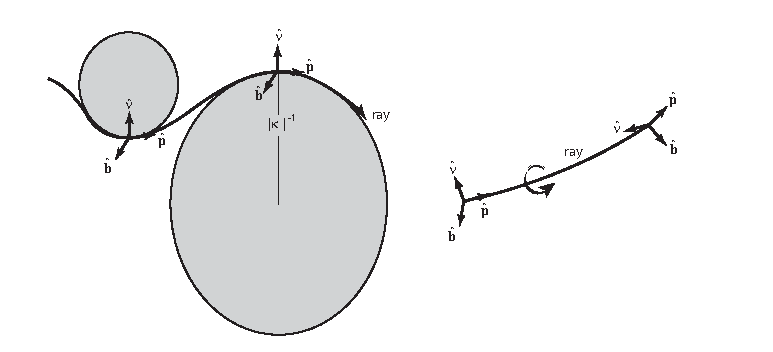
\includegraphics{../figures/chap15/fig01.eps}
\end{center}
\caption[curvature&torsion]
{\label{15.fig.curtor}
Schematic depiction of the curvature $\kappa$ and
torsion $\tau$ of a seismic ray.  The unit slowness
vector $\hat{\bf p}$ is everywhere tangent to the ray.
({\em Left}) The ray normal $\hat{\mbox{\boldmath $\nu$}}$
points either toward or away from the center
of curvature of the shaded tangent circle,
which lies within the osculating plane.
The radius of the circle is the absolute
reciprocal $|\kappa|^{-1}$ of the curvature.
({\em Right}) The torsion $\tau$ is
the arclength rate at which the normal
$\hat{\mbox{\boldmath $\nu$}}$ and
binormal $\hat{\bf b}=\hat{\bf p}
\times\hat{\mbox{\boldmath $\nu$}}$ twist in
a right-hand sense about the ray.}
\end{figure}
The curvature $\kappa$ and torsion $\tau$ may be written
explicitly in terms of the first three derivatives of the
position vector $\bx(s)$ in the form
\eq \label{15.kappadef}
\kappa^2=\frac{d^2\bx}{ds^2}\cdot
\frac{d^2\bx}{ds^2},
\en
\eq \label{15.tordef}
\tau=\kappa^{-2}\left(\frac{d\bx}{ds}
\cdot\frac{d^2\bx}{ds^2}\times
\frac{d^3\bx}{ds^3}\right).
\en
Equations~(\ref{15.Frenet})--(\ref{15.tordef})
pertain to any smooth curve in three-dimensional space;
by combining these geometrical results with
the ray-tracing equation~(\ref{15.raypath2}),
we can express the curvature and torsion of a
seismic ray in terms of the logarithmic gradients of
the wave speed:
\eq \label{15.kappatau}
\kappa=-\bnuh\cdot\bdel(\ln v),\qquad
\tau=-\kappa^{-1}\hat{\bp}\cdot\bdel\bdel(\ln v)\cdot\hat{\bb}.
\en
A ray twists in such a way that its normal $\bnuh$ is always
parallel and its binormal $\hat{\bb}$ is always perpendicular
to the cross-path gradient:
\eq \label{15.Frenlast}
\bnuh=-\kappa^{-1}\bdel_{\!\perp}(\ln v),\qquad
\hat{\bb}\cdot\bdel_{\!\perp}(\ln v)=0.
\en
With our sign convention, $\bnuh$ points in the direction
of decreasing wave speed wherever the curvature $\kappa$
is positive, and in the direction of increasing wave speed
wherever it is negative.  We illustrate the evolution
of the Serret-Fr\'{e}net triad $\hat{\bp}$, $\bnuh$, $\hat{\bb}$
along a seismic ray in Figure~\ref{15.fig.curtor}.
\index{ray tracing!kinematic!body waves|)}%
\index{ray tracing!body-wave|)}%
\index{Serret-Fr\'{e}net formulae|)}%
\index{body-wave polarization|)}%
\index{polarization!body-wave|)}%

\section{Amplitude Variation}
\index{amplitude!body-wave|(}%
\index{body-wave amplitude|(}%

The ray-tracing equations discussed above enable us to
determine the ray trajectories and the variations in
travel time $T_{\rm P}$ or $T_{\rm S}$ along them.
The transport equations~(\ref{15.transport}),
which we consider next, determine the variations
in amplitude $A_{\rm P}$ or $A_{\rm S}$ along
the rays.  Dropping the identifying subscripts P and S,
as before, we rewrite~(\ref{15.transport})
in the generic form
\eq \label{15.gtrans}
\bdel\cdot\bsK=0,
\en
where
\eq \label{15.genKdef}
\bsK=v\sE\hat{\bp}=\om^2\rho vA^2\hat{\bp}
=\om^2\rho v^2A^2\bp.
\en
Equation~(\ref{15.gtrans}) can be solved for the amplitude
variation $A$ along a ray in a variety of ways;
we describe several of these methods and indicate
the relations between them in the following sections.
Amplitude determination is an important consideration in a
variety of applications, including wavefront extrapolation;
we take a relatively limited view, restricting attention to
the waves emitted by a point source. 

\subsection{Conservation of energy}
\index{conservation!of body-wave energy|(}%
\index{energy!conservation of!body-wave|(}%

We begin by noting that the differential
relation $\bdel\cdot\bsK=0$ has an obvious
physical interpretation---it expresses the {\em conservation
of body-wave energy\/}.  This can be seen by considering
an infinitesimally narrow tube of trajectories surrounding
a ray path from $\bx_1$ to $\bx_2$, as shown in Figure~12.7.
Let $V$ be the volume of this ray-tube segment, and denote
the outward unit normal on the boundary surface $\p V$
(temporarily) by $\bnuh$.  Upon integrating~(\ref{15.gtrans})
over $V$ and invoking Gauss' theorem, we obtain
\eq \label{15.enercon}
\int_V\bdel\cdot\bsK\,dV=\int_{\spar V}\bnuh\cdot\bsK\,d\/\Sigma
=\|\bsK\|_2\,d\/\Sigma_2-\|\bsK\|_1\,d\/\Sigma_1=0,
\en
where $d\/\Sigma_1$ and $d\/\Sigma_2$ are the differential
areas of the cross-sectional patches at $\bx_1$ and $\bx_2$,
respectively, and we have used the fact that $\bnuh\cdot\bsK=0$
on the sidewalls of the ray tube.  All of the wave energy that
enters the ray tube at $\bx_1$ leaves it at $\bx_2$; there is
no energy leakage through the sidewalls nor absorption within
the perfectly elastic ray tube.  Equation~(\ref{15.enercon})
yields the amplitude variation relation~(\ref{12.ampratio}),
which we repeat here for convenience:
\eq \label{15.amplaw}
\frac{A_2}{A_1}=\left(\frac{\rho_2v_2}
{\rho_1v_1}\right)^{-1/2}\left|\frac{d\/\Sigma_2}
{d\/\Sigma_1}\right|^{-1/2}.
\en
The absolute value is necessary to account for the
change in sign of the differential area of a ray tube
upon passage through a caustic or focal point, as we
discuss in Sections~12.1.8 and~15.4.3.
\index{conservation!of body-wave energy|)}%
\index{energy!conservation of!body-wave|)}%

\renewcommand{\thesubsection}{$\!\!\!\raise1.3ex\hbox{$\star$}\!\!$
\arabic{chapter}.\arabic{section}.\arabic{subsection}}
\subsection{Ray-tube area}
\index{ray-tube area|(}%
\renewcommand{\thesubsection}{\arabic{chapter}.\arabic{section}.\arabic{subsection}}

Following Kline \& Kay ({\citeyear{kline&kay79}) we can
obtain an explicit expression for the ray-tube area ratio
$d\/\Sigma_2/d\/\Sigma_1$ in equation~(\ref{15.amplaw}).
Consider the volume integral
\eq \label{15.kline1}
\int_V\bdel\cdot\hat{\bp}\;dV=\int_{\spar V}\bnuh\cdot\hat{\bp}\;d\/\Sigma
=d\/\Sigma_2-d\/\Sigma_1,
\en
where the final equality is valid because $V$ is an infinitesimally
narrow ray tube.  We can also express the left side
of~(\ref{15.kline1}) as a line integral along the trajectory
from $\bx_1$ to $\bx_2$:
\eq \label{15.kline2}
\int_V\bdel\cdot\hat{\bp}\;dV=
\int_{s_1}^{s_2}\bdel\cdot\hat{\bp}\;d\/\Sigma\;ds,
\en
where $d\/\Sigma(s)$ is the differential area at a running point
along the ray.  Upon comparing equations~(\ref{15.kline1})
and~(\ref{15.kline2}) we deduce that
\eq \label{15.kline3}
d\/\Sigma_2-d\/\Sigma_1=
\int_{s_1}^{s_2}\bdel\cdot\hat{\bp}\;d\/\Sigma\;ds.
\en
The solution to this linear integral equation is
\eq \label{15.kline4}
\frac{d\/\Sigma_2}{d\/\Sigma_1}=\exp\left(\int_{s_1}^{s_2}
\bdel\cdot\hat{\bp}\;ds\right).
\en
The integrand in equation~(\ref{15.kline4})
is the sum of the principal curvatures of the wavefront
at a point $s$ along the ray:
\eq \label{15.Gausscurv}
\bdel\cdot\hat{\bp}=\frac{1}{R_1}+\frac{1}{R_2}.
\en
The quantities $R_1$ and $R_2$ are the corresponding
{\em radii of curvature\/}.
\index{radius of curvature}%

Yet another expression for $d\/\Sigma_2/d\/\Sigma_1$ can be
obtained by rewriting the transport equation
$\bdel\cdot(\rho v^2A^2\bp)=0$ in the form
\eq \label{15.gtrans2}
\frac{d}{d\/\sigma}\ln(\rho v^2A^2)=-\bdel\cdot\bp,
\en
where we have used the fact that
$\bp\cdot\bdel=(d\bx/\hspace{-0.3 mm}d\sigma)\cdot\bdel
=d/\hspace{-0.3 mm}d\sigma$ along a ray.
The energy conservation law $\rho vA^2\,d\/\Sigma
={\rm constant}$ enables us
to convert this into a differential equation for
the ray-tube area:
\eq \label{15.dSigeqn}
\frac{d}{d\/\sigma}\ln(v^{-1}d\/\Sigma)=\bdel\cdot\bp.
\en
This equation can be integrated to yield the result
\eq \label{15.dSigeqn2}
\frac{d\/\Sigma_2}{d\/\Sigma_1}=\frac{v_2}{v_1}
\exp\left(\int_{\sigma_1}^{\sigma_2}
\bdel\cdot\bp\;d\sigma\right).
\en
The integrand $\bdel\cdot\bp$ in this case
is the {\em Laplacian of the travel time\/}
at a point $\sigma$ along the ray:
\eq
\bdel\cdot\bp=\del^2T.
\en
The previous
result~(\ref{15.kline4}) can be deduced from~(\ref{15.dSigeqn2})
by substituting $\bdel\cdot\bp=\bdel\cdot(v^{-1}\bph)
=v^{-1}\bdel\cdot\hat{\bp}-d(\ln v)/\hspace{-0.3 mm}d\sigma$.
\index{ray-tube area|)}%

\subsection{Point-source Jacobian}
\index{Jacobian!point-source!body waves|(}%
\index{point-source Jacobian!body waves|(}%

Only two parameters are needed to characterize the initial
takeoff direction of a ray from a fixed point source
\index{takeoff angle}%
$\bx'$.  For the time being, it is unnecessary to
adopt a specific choice for these parameters; we shall
refer to them as $\gamma^{\prime}_1$ and $\gamma^{\prime}_2$,
where the primes serve as a reminder that they are measured
at the point $\bx'$.  A given point in the ensemble of
all rays shot from $\bx'$ may be
regarded as a function of the form
$\bx=\bx(\sigma,\gamma^{\prime}_1,\gamma^{\prime}_2)$,
where $\gamma^{\prime}_1$, $\gamma^{\prime}_2$ identify
the ray and $\sigma$ specifies the position along it.
The partial derivatives with respect to the ray parameters
$\p_{\gamma^{\prime}_1}\bx
=(\p\bx/\p\gamma^{\prime}_1)_{\sigma,\gamma^{\prime}_2}$
and $\p_{\gamma^{\prime}_2}\bx=
(\p\bx/\p\gamma^{\prime}_2)_{\sigma,\gamma^{\prime}_1}$
both lie within the instantaneous
wavefront passing through the point $\bx$;
the condition that guarantees this is
\eq \label{15.dgamperp}
\bp\cdot\p_{\gamma^{\prime}}\bx=0,
\en
where $\gamma'$ denotes either $\gamma^{\prime}_1$ or
$\gamma^{\prime}_2$.  The area of an infinitesimally narrow
ray tube is given in terms of the differentials $d\gamma^{\prime}_1$
and $d\gamma^{\prime}_2$ by the classical geometrical relation
(Willmore \citeyear{willmore59}):
\eq \label{15.classdSig}
d\/\Sigma=\hat{\bp}\cdot
(\p_{\gamma^{\prime}_1}\bx\times\p_{\gamma^{\prime}_2}\bx)
\,d\gamma^{\prime}_1\,d\gamma^{\prime}_2.
\en
The cross product $\p_{\gamma^{\prime}_1}\bx\times\p_{\gamma^{\prime}_2}\bx$
in~(\ref{15.classdSig}) is either parallel or anti-parallel to the
direction of propagation $\hat{\bp}$, depending upon the sign
of $d\/\Sigma$.

We define the {\em point-source Jacobian\/} to be the determinant
\index{point-source Jacobian!body waves}%
\index{Jacobian!point-source!body waves}%
\eq \label{15.Jacob1}
J=\frac{\p(x_1,x_2,x_3)}{\p(\sigma,\gamma^{\prime}_1,\gamma^{\prime}_2)}
={\rm det}\left(\begin{array}{ccc}
\displaystyle{\frac{\p x_1}{\p\sigma}} &
\displaystyle{\frac{\p x_1}{\p\gamma^{\prime}_1}} &
\displaystyle{\frac{\p x_1}{\p\gamma^{\prime}_2}} \\
\vspace{-2.0 mm} && \\
\displaystyle{\frac{\p x_2}{\p\sigma}} &
\displaystyle{\frac{\p x_2}{\p\gamma^{\prime}_1}} &
\displaystyle{\frac{\p x_2}{\p\gamma^{\prime}_2}} \\
\vspace{-2.0 mm} && \\
\displaystyle{\frac{\p x_3}{\p\sigma}} &
\displaystyle{\frac{\p x_3}{\p\gamma^{\prime}_1}} &
\displaystyle{\frac{\p x_3}{\p\gamma^{\prime}_2}} \\
\end{array}\right).
\en
This can be expanded with the aid of the kinematic
relation $d\bx/\hspace{-0.3 mm}d\sigma=\bp$:
\eq \label{15.Jacob2}
J=\bp\cdot(\p_{\gamma^{\prime}_1}\bx\times\p_{\gamma^{\prime}_2}\bx).
\en
The quantities $d\/\Sigma$ and $J$ change sign in unison,
and are related at all points along a ray by
\eq \label{15.Jacob3}
d\/\Sigma=vJ\,d\gamma^{\prime}_1\,d\gamma^{\prime}_2.
\en
In other words, $vJ$ is the Jacobian that relates the
differential ray-tube area $d\/\Sigma$ to the ray
parameters $\gamma^{\prime}_1$ and $\gamma^{\prime}_2$.
The absolute value of $J$ can be written in the form
\eq \label{15.Jacob4}
|J|=v^{-1}\|\p_{\gamma^{\prime}_1}\bx\times\p_{\gamma^{\prime}_2}\bx\|
=v^{-1}\sqrt{EG-F^2},
\en
where we have let
\eq
E=\p_{\gamma^{\prime}_1}\bx\cdot\p_{\gamma^{\prime}_1}\bx,\quad\;\;
G=\p_{\gamma^{\prime}_2}\bx\cdot\p_{\gamma^{\prime}_2}\bx,\quad\;\;
F=\p_{\gamma^{\prime}_1}\bx\cdot\p_{\gamma^{\prime}_2}\bx.
\en
Upon replacing the independent variable $\sigma$
in~(\ref{15.Jacob1}) by $s$ and $T$, we obtain the
alternative point-source Jacobians $J'=vJ$ and
$J''=v^2J$.  The former is used as the basis of
ray-amplitude calculations by many authors
(e.g., \v{C}erven\'{y} \citeyear{cerveny85})
because of the convenient interpretation $d\/\Sigma
=J'\,d\gamma^{\prime}_1\,d\gamma^{\prime}_2$.
\index{Jacobian!point-source!body waves|)}%
\index{point-source Jacobian!body waves|)}%

\renewcommand{\thesubsection}{$\!\!\!\raise1.3ex\hbox{$\star$}\!\!$
\arabic{chapter}.\arabic{section}.\arabic{subsection}}
\subsection{Smirnov's lemma}
\index{Smirnov's lemma|(}%
\renewcommand{\thesubsection}{\arabic{chapter}.\arabic{section}.\arabic{subsection}}

A general method of solving the transport equation~(\ref{15.gtrans}) is based
upon a mathematical result described by Smirnov (\citeyear{smirnov64}) and
Thomson \& Chapman (\citeyear{thomson&chapman85}), which we reiterate here.
Smirnov's lemma states that
\eq \label{15.smirnov}
\frac{d}{d\sigma}(\ln J)=\bdel\cdot\bp\quad
\mbox{whenever}\quad \frac{d{\bf x}}{d\sigma}=\bp.
\en
To prove~(\ref{15.smirnov}) we consider the quantity
\eq \label{15.proof}
\frac{dJ}{d\sigma}=
\frac{\p(p_1,x_2,x_3)}{\p(\sigma,\gamma^{\prime}_1,\gamma^{\prime}_2)}
+\frac{\p(x_1,p_2,x_3)}{\p(\sigma,\gamma^{\prime}_1,\gamma^{\prime}_2)}
+\frac{\p(x_1,x_2,p_3)}{\p(\sigma,\gamma^{\prime}_1,\gamma^{\prime}_2)},
\en
where $p_i=dx_i/\hspace{-0.3 mm}d\sigma$.
The sum of three determinants~(\ref{15.proof})
can be expanded into a sum of nine determinants
by means of the substitutions
\eq
\frac{\p p_i}{\p\sigma}
=\frac{\p p_i}{\p x_j}\frac{\p x_j}{\p\sigma},\qquad
\frac{\p p_i}{\p\gamma^{\prime}_1}
=\frac{\p p_i}{\p x_j}\frac{\p x_j}{\p\gamma^{\prime}_1},\qquad
\frac{\p p_i}{\p\gamma^{\prime}_2}
=\frac{\p p_i}{\p x_j}\frac{\p x_j}{\p\gamma^{\prime}_2}.
\en
However, six of these nine determinants are
identically zero, because their rows are linearly
dependent.  The remaining three determinants can be combined to give
\eq \label{15.proof2}
\frac{dJ}{d\sigma}=
\bigg(\frac{\p p_j}{\p x_j}\bigg)
\frac{\p(x_1,x_2,x_3)}{\p(\sigma,\gamma^{\prime}_1,\gamma^{\prime}_2)}
=(\bdel\cdot\bp)\hspace{0.3 mm}J,
\en
which is the desired result~(\ref{15.smirnov}).

It is a straightforward matter to apply Smirnov's lemma;
upon combining~(\ref{15.smirnov}) and~(\ref{15.gtrans2})
we deduce that
\eq \label{15.gtrans3}
\frac{d}{d\/\sigma}\ln(\rho v^2A^2J)=0.
\en
Equation~(\ref{15.gtrans3}) enables us to express
the ratio of the amplitudes at two consecutive
points $\bx_1$ and $\bx_2$ along a ray in terms
of a ratio of Jacobians:
\eq \label{15.amplaw3}
\frac{A_2}{A_1}=\left(\frac{\rho_2v_2^2}
{\rho_1v_1^2}\right)^{-1/2}\left|\frac{J_2}{J_1}\right|^{-1/2}.
\en
Of course, we could have obtained the result~(\ref{15.amplaw3})
from~(\ref{15.amplaw}) by making use of the identification~(\ref{15.Jacob3}).
However, Smirnov's lemma can be formulated and applied in a wide variety
of other settings, as we shall see
in Sections~15.8.8} and~\ref{section:16.4.4}.
\index{Smirnov's lemma|)}%

\subsection{Geometrical spreading factor}
\index{geometrical spreading factor!body waves|(}%

As in the case of a spherically symmetric Earth,
we define a positive {\em geometrical spreading factor\/}
\index{geometrical spreading factor}%
$\sR(\bx,\bx')$, which is analogous to the source-receiver
distance $\|\bx-\bx'\|$ in a homogeneous medium, by
\eq \label{15.sRdef}
\sR=\sqrt{|d\/\Sigma|/d\/\Omega},
\en
where $d\/\Omega$ is the differential solid angle subtended by
the ray tube at the source $\bx'$.  We can express this solid
angle in terms of the partial derivatives of
the unit slowness $\hat{\bp}'$ at the source in the form:
\eq \label{15.dOmega}
d\/\Omega=\hat{\bp}'\cdot(\p_{\gamma^{\prime}_1}\hat{\bp}'\times
\p_{\gamma^{\prime}_2}\hat{\bp}')\,d\gamma^{\prime}_1\,d\gamma^{\prime}_2
=\|\p_{\gamma^{\prime}_1}\hat{\bp}'\times
\p_{\gamma^{\prime}_2}\hat{\bp}'\|\,d\gamma^{\prime}_1\,d\gamma^{\prime}_2.
\en
The spreading factor is therefore related to the Jacobian~(\ref{15.Jacob1}) by
\eq \label{15.sRdef2}
\sR=\sqrt{\frac{v|J|}{\|\p_{\gamma^{\prime}_1}\hat{\bp}'\times
\p_{\gamma^{\prime}_2}\hat{\bp}'\|}}=
\sqrt{\frac{\|\p_{\gamma^{\prime}_1}\bx\times
\p_{\gamma^{\prime}_2}\bx\|}
{\|\p_{\gamma^{\prime}_1}\hat{\bp}'\times
\p_{\gamma^{\prime}_2}\hat{\bp}'\|}}.
\en
Equation~(\ref{15.kline4}) can be used to obtain another expression
for the spreading factor, as a line integral along a ray:
\eq \label{15.sRdef3}
\sR=\lim_{s'\rightarrow 0}s'\left|\exp\left(\half
\int_{s'}^s\bdel\cdot\hat{\bp}\;ds\right)\right|,
\en
where we have used the limiting relation
$d\/\Sigma'\rightarrow s^{\prime 2}d\/\Omega$
in the vicinity of the source, $s'\rightarrow 0$.
The outgoing wavefront in a homogeneous medium is
a sphere with surface divergence
$\bdel\cdot\hat{\bp}=2s^{-1}$, so that~(\ref{15.sRdef3})
reduces to $\sR=s=\|\bx-\bx'\|$, as expected.
\index{geometrical spreading factor!body waves|)}%

\subsection{Dynamical reciprocity}
\index{reciprocity!geometrical spreading factor|(}%
\label{15.sec.Backus}

Let us rewrite the differential-area and solid-angle
relationships~(\ref{15.classdSig}) and~(\ref{15.dOmega})
in terms of $\bp=v^{-1}\hat{\bp}$ using index notation:
\eq \label{15.Backus1}
d\/\Sigma=v\eps_{imn}\,p_i(\p_{\gamma^{\prime}_1}x_m)
(\p_{\gamma^{\prime}_2}x_n)\,d\gamma^{\prime}_1
\,d\gamma^{\prime}_2,
\en
\eq \label{15.Backus2}
d\/\Omega=v^{\prime 3}\eps_{jkl}\,p^{\prime}_j
(\p_{\gamma^{\prime}_1}p^{\prime}_k)
(\p_{\gamma^{\prime}_2}p^{\prime}_l)\,d\gamma^{\prime}_1
\,d\gamma^{\prime}_2.
\en
Upon regarding the travel time as a function $T(\bx,\bx')=T(\bx',\bx)$ of
{\em both\/} endpoints, we can express the slowness derivatives
$\p_{\gamma^{\prime}}\bp'$ in terms of $\p_{\gamma^{\prime}}\bx$
in the form $\p_{\gamma^{\prime}}\bp'=-\p_{\gamma^{\prime}}\bx
\cdot\bdel\bdel^{\prime}T$.
Substituting this into~(\ref{15.Backus2})
we obtain
\eq \label{15.Backus3}
d\/\Omega=v^{\prime 3}\eps_{jkl}\,p^{\prime}_j
(\p_{\gamma^{\prime}_1}x_m)(\p_m\p^{\prime}_kT)
(\p_{\gamma^{\prime}_2}x_n)(\p_n\p^{\prime}_lT)
\,d\gamma^{\prime}_1 \,d\gamma^{\prime}_2.
\en
It is convenient to introduce a tensor function of the two endpoints:
\eq \label{15.Backus4}
\bS(\bx,\bx')=({\rm det}\,\bdel\bdel^{\prime}T)
(\bdel\bdel^{\prime}T)^{-1}=\bS^{\rm T}(\bx',\bx).
\en
The components of~(\ref{15.Backus4}) are given by
Cramer's rule~(\ref{A.Cramrule}):
\eq
S_{ij}(\bx,\bx')=S_{ji}(\bx',\bx)
=\half\eps_{imn}\eps_{jkl}(\p_m\p^{\prime}_kT)(\p_n\p^{\prime}_lT).
\en
The easily verified relationship
$\eps_{imn}S_{ij}=\eps_{jkl}(\p_m\p^{\prime}_kT)(\p_n\p^{\prime}_lT)$
enables us to write $d\/\Omega$ in terms of $d\/\Sigma$ in the form
\eq \label{15.Backus5}
d\/\Omega=v^{\prime 3}\eps_{imn}\,p^{\prime}_jS_{ij}
(\p_{\gamma^{\prime}_1}x_m)(\p_{\gamma^{\prime}_2}x_n)
=vv^{\prime 3}p_iS_{ij}p^{\prime}_j\,d\/\Sigma.
\en
Reverting to invariant notation, we obtain another explicit expression
for the geometrical spreading factor $\sR=\sqrt{|d\/\Sigma|/
\hspace{-0.3 mm}d\/\Omega}\,$:
\index{geometrical spreading factor!body waves}%
\eq \label{15.Backus6}
v(\bx')\sR(\bx,\bx')=|\hat{\bp}\cdot\bS(\bx,\bx')\cdot\hat{\bp}'|^{-1/2}.
\en
The symmetry~(\ref{15.Backus4}) renders the right side of~(\ref{15.Backus6})
invariant under an interchange of the source and receiver:
\eq \label{15.Backus7}
\bx\rightarrow\bx',\qquad\bx'\rightarrow\bx,\qquad
\hat{\bp}\rightarrow-\hat{\bp}',\qquad
\hat{\bp}'\rightarrow-\hat{\bp}.
\en
It follows that $\sR$ satisfies the dynamical symmetry or
{\em reciprocity relation\/}
\eq \label{15.Backus8}
v(\bx')\sR(\bx,\bx')=v(\bx)\sR(\bx',\bx).
\en
Equation~(\ref{15.Backus8}) is identical to the relation governing
geometrical spreading within a spherically symmetric Earth;
see Section~\ref{12.sec.spread}.  The above geometrical
argument, which generalizes this result to an arbitrary
Earth, is given by Richards (\citeyear{richards71});
he attributes the proof to G.\ E.\ Backus.

A physical interpretation of the wave-speed factors $v(\bx)$
and $v(\bx')$ in the reciprocity relation~(\ref{15.Backus8})
is given by Snieder \& Chapman (\citeyear{snieder&chapman98}).
Suppose the source $\bx'$ lies directly below the receiver
$\bx$ in a medium whose speed depends only upon depth.
If $v(\bx')>v(\bx)$, the rays shot upward from $\bx'$
diverge more slowly than the rays shot downward from $\bx$,
because rays are refracted away from high wave speeds.
The spreading factor from the source to the receiver
must therefore be less than that from the receiver to
the source: $\sR(\bx,\bx')<\sR(\bx',\bx)$.  This simple
example shows why ``pure'' reciprocity $\sR(\bx,\bx')=
\sR(\bx',\bx)$ of the geometrical spreading does not hold.
\index{reciprocity!geometrical spreading factor|)}%

\subsection{Caustics and focal points}
\index{caustic!body waves|(}%
\index{focal point|(}%
\label{15.sec.Maslov}

Singular points along a ray where the differential
area $d\/\Sigma$ vanishes are referred to
as {\em caustics\/} or {\em focal points\/}.
These two types of ray singularities are distinguished
by the number of transverse dimensions in which
the ray tube ``collapses'' simultaneously, as
illustrated in Figure~12.8.
Only one of the radii of curvature of the associated
wavefront vanishes at a caustic, whereas both
vanish at a focal point:
\eq \label{15.causfocdef}
\begin{array}{ll}
\mbox{caustic:} & R_1R_2=0, \\
\mbox{focal~point:} & R_1=R_2=0.
\end{array}
\en
The ray-tube area $d\/\Sigma$ undergoes a change in
sign upon passage through a caustic; upon passing
through a focal point, it may be considered to change
sign twice, so that its original sign is retained.
Focal points are a design feature of telescopes
and many other man-made imaging devices; however,
they are extremely rare in seismology.  Caustics,
on the other hand, are a ubiquitous feature of
seismic rays in strongly heterogeneous media.
In three-dimensional space, the caustics lie on two-dimensional
surfaces that are {\em envelopes\/} of the ray field.
\index{envelope of rays}%
In addition to simple fold and cusp caustics, there
are a number of other more complex types; the possible
morphologies can be characterized using catastrophe
theory (Poston \& Stewart \citeyear{poston&stewart78}).
We do not discuss the morphological classification of these so-called
{\em diffraction catastrophes\/}
\index{diffraction catastrophe}%
here; detailed treatments
may be found in Berry \& Upstill (\citeyear{berry&upstill80})
and Kravtsov \& Orlov (\citeyear{kravtsov&orlov90}).

The phase of a wave undergoes a non-geometrical
$\pi/2$ phase advance upon every passage through
a caustic, as discussed in Section~12.1.8.  To keep
track of these cumulative phase shifts, we introduce
the {\em Maslov index\/},
\index{Maslov index!body waves}%
\index{index!Maslov}%
a positive integer counter
which starts at $M=0$ and increases by one every time
that a ray passes through a caustic.  Rare passages
through a focal point increase the Maslov index by two.
The location and structure of the
caustic surfaces or envelopes of the rays
leaving a source $\bx'$ and receiver $\bx$
are obviously different, but the number of
caustic passages along every ray and reversed
ray is the same:
\eq \label{15.Mrecip}
M(\bx',\bx)=M(\bx,\bx').
\en
A proof of this {\em Maslov reciprocity principle\/}
\index{Maslov reciprocity principle}%
\index{reciprocity!Maslov index}%
can be based upon the observation that $M$ is the number
of sign changes of the differential area $d\/\Sigma$ along
a ray; the considerations in Section~\ref{15.sec.Backus}
show that this number is independent of the direction
in which the ray is traced.
\index{caustic!body waves|)}%
\index{focal point|)}%

\subsection{Dynamical ray tracing}
\index{ray tracing!body-wave|(}%
\index{body-wave ray tracing|(}%
\index{dynamical ray tracing!body waves|(}%

We can calculate the partial derivatives
needed to evaluate~(\ref{15.sRdef2}) by differentiating Hamilton's 
equations~(\ref{15.Hameqn}) with respect to the ray parameters
$\gamma'=\gamma^{\prime}_1,\gamma^{\prime}_2$.  This results in
a system of linear equations governing the twelve derivatives
$\p_{\gamma^{\prime}}\bx$ and $\p_{\gamma^{\prime}}\bp$:
\eq \label{15.12eqns}
\frac{d}{d\sigma}\left(\!\begin{array}{c}
\p_{\gamma^{\prime}}\bx \\
\vspace{-2.0 mm} \\
\p_{\gamma^{\prime}}\bp
\end{array}\!\right)=\left(\begin{array}{rr}
\p_{\subp}\p_{\subx}H  & \p_{\subp}\p_{\subp}H  \\
\vspace{-2.0 mm}  & \\
-\p_{\subx}\p_{\subx}H  &
-\p_{\subx}\p_{\subp}H 
\end{array}\right)\cdot\left(\!\begin{array}{c}
\p_{\gamma^{\prime}}\bx \\
\vspace{-2.0 mm} \\
\p_{\gamma^{\prime}}\bp
\end{array}\!\right).
\en
For future reference, we denote the six-dimensional tensor
on the right side of~(\ref{15.12eqns}) by
\eq \label{15.6Adef}
\bA=\left(\begin{array}{rr}
\p_{\subp}\p_{\subx}H  & \p_{\subp}\p_{\subp}H  \\
\vspace{-2.0 mm}  & \\
-\p_{\subx}\p_{\subx}H  & -\p_{\subx}\p_{\subp}H 
\end{array}\right)=\left(\begin{array}{cc}
\bzero  & \bI  \\
\vspace{-2.0 mm}  & \\
\half\bdel\bdel v^{-2}  & \bzero
\end{array}\right).
\en
The rays leaving a point source are characterized
by two requirements:
\eq \label{15.ptconstr}
\p_{\gamma^{\prime}}\bx'=\bzero\quad\mbox{and}\quad
\bp'\cdot\p_{\gamma^{\prime}}\bp'=0.
\en
In accordance with~(\ref{15.ptconstr}), we must integrate~(\ref{15.12eqns})
subject to the initial conditions
\eq \label{15.12inconds}
\p_{\gamma^{\prime}}\bx(0)=\bzero,\qquad
\p_{\gamma^{\prime}}\bp(0)=(\bI-\hat{\bp}'\hat{\bp}')
\cdot\p_{\gamma^{\prime}}\bp'.
\en
The two vectors $\bx+\p_{\gamma^{\prime}}\bx$ and $\bp+\p_{\gamma^{\prime}}\bp$
are the position and slowness along a pair of {\em neighboring or paraxial
rays\/},
\index{neighboring ray}%
\index{paraxial ray}%
as illustrated in Figure~\ref{15.fig.neighbor}.
\begin{figure}
\begin{center}
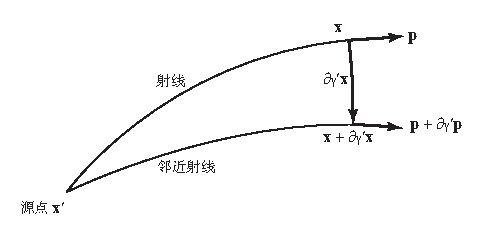
\includegraphics{../figures/chap15/fig02.eps}
\end{center}
\caption[paraxial ray]
{\label{15.fig.neighbor}
Schematic depiction of a central and neighboring or paraxial ray
shot from a source ${\bf x}'$.  The position vectors ${\bf x}$
and ${\bf x}+\partial_{\gamma'}{\bf x}$ are situated at the
same value of $\sigma$ along the two rays.  The differential
vector $\partial_{\gamma'}{\bf x}$ therefore lies within the
wavefront.  Wavefront curvature causes the central and paraxial
slownesses ${\bf p}$ and ${\bf p}+\partial_{\gamma'}{\bf p}$ to
be misaligned.}
\end{figure}
Equations~(\ref{15.12eqns}) are referred to as the
{\em dynamic ray-tracing equations\/}, to distinguish
\index{ray tracing!dynamical}%
them from the kinematic equations~(\ref{15.Hameqn}).
Alternative forms of these equations with the
independent variable $\sigma$ replaced by either $s$ or $T$ and the
Hamiltonian $H$ replaced by $H'$ or $H''$ are easy to obtain.

Equation~(\ref{15.dgamperp}) imposes a constraint upon the solutions
$\p_{\gamma^{\prime}}\bx$, $\p_{\gamma^{\prime}}\bp$ to the dynamic
ray-tracing equations.  Differentiation of the eikonal
equation~(\ref{15.Heqzero}) yields another:
\eqa \label{15.dxdpeqn} \lefteqn{
\p_{\gamma^{\prime}}H=\p_{\gamma^{\prime}}\bx\cdot\p_{\subx}H+
\p_{\gamma^{\prime}}\bp\cdot\p_{\subp}H} \nonumber \\
&&\mbox{}\hspace{1.0 mm}
=-\half\p_{\gamma^{\prime}}\bx\cdot\bdel v^{-2}
+\p_{\gamma^{\prime}}\bp\cdot\bp=0.
\ena
Imposition of the two conditions~(\ref{15.ptconstr})
at the source $\sigma=0$ guarantees that~(\ref{15.dgamperp})
and~(\ref{15.dxdpeqn}) are both satisfied for all $\sigma>0$.
Just as in the kinematic case,
it is possible to use the constraints~(\ref{15.dgamperp})
and~(\ref{15.dxdpeqn}) to reduce~(\ref{15.12eqns}) to a
system of eight rather than twelve dynamic ray-tracing
equations in ray-centered coordinates (\v{C}erven\'{y}
\citeyear{cerveny85}; Farra \& Madariaga \citeyear{farra&madariaga87}).
We present an alternative system of eight dynamical equations in
Section~\ref{15.sec.jeroen2}.
\index{ray tracing!body-wave|)}%
\index{body-wave ray tracing|)}%
\index{dynamical ray tracing!body waves|)}%

\renewcommand{\thesubsection}{$\!\!\!\raise1.3ex\hbox{$\star$}\!\!$
\arabic{chapter}.\arabic{section}.\arabic{subsection}}
\subsection{Phase-space propagator}
\index{phase-space propagator|(}%
\index{propagator!phase-space|(}%
\renewcommand{\thesubsection}{\arabic{chapter}.\arabic{section}.\arabic{subsection}}

More general solutions to the dynamical
ray-tracing equations~(\ref{15.12eqns}), with
arbitrary initial conditions, may be written in terms
of the {\em propagator\/} $\bP(\sigma,0)$
\index{propagator matrix}%
\index{matrix!propagator}%
between the origin and a point $\sigma$ along a ray, defined by
(Gilbert \& Backus \citeyear{gilbert&backus66})
\eq \label{15.propdef}
\frac{d{\bf P}}{d\sigma}=\bA\cdot\bP,\qquad
\bP(0,\sigma)\cdot\bP(\sigma,0)
=\bP(0,0)=\bI.
\en
The elements of this six-dimensional propagator are the
thirty-six partial derivatives of the final
position and slowness
coordinates with respect to the initial ones:
\eq \label{15.propdef2}
\bP(\sigma,0)=\left(\begin{array}{ccc}
\displaystyle{\frac{\p x_1}{\p x^{\prime}_1}} &
\cdots & \displaystyle{\frac{\p x_1}{\p p^{\prime}_3}} \\
\vspace{-3.0 mm} && \\
\vdots && \vdots \\
\vspace{-3.0 mm} && \\
\displaystyle{\frac{\p p_3}{\p x^{\prime}_1}} &
\cdots & \displaystyle{\frac{\p p_3}{\p p^{\prime}_3}}
\end{array}\right).
\en
As in any phase-space analysis, the initial position $\bx'$ and
slowness $\bp'$ are regarded as {\em independent\/} variables.
A given term such as the one
in the upper right corner is thus of the form
$(\p x_1/\p p^{\prime}_3)_{x_1,x_2,x_3,p^{\prime}_1,p^{\prime}_2,\sigma}$.
It is convenient to write~(\ref{15.propdef2})
in terms of four three-dimensional sub-propagators:
\eq \label{15.Pdecomp}
\bP=\left(\begin{array}{cc}
\bX_{\subx} & \bX_{\subp} \\
\vspace{-2.0 mm} & \\
\bP_{\subx} & \bP_{\subp} \end{array}\right).
\en
The upper-right term $\bX_{\subp}$ is the only one that is required to
find the Jacobian~(\ref{15.Jacob1}) and geometrical spreading
factor~(\ref{15.sRdef2}) of a point source:
\eq \label{15.ptsrcsol}
\p_{\gamma^{\prime}}\bx=\bX_{\subp}\cdot
(\bI-\hat{\bp}'\hat{\bp}')\cdot\p_{\gamma^{\prime}}\bp'.
\en
Of course, it is not possible to solve for $\bX_{\subp}$ alone,
since it is coupled to the other three-dimensional propagators
$\bX_{\subx}$, $\bP_{\subx}$ and $\bP_{\subp}$.

It is easily demonstrated by means of an argument similar to that in
Section~15.4.4 that the determinant of the phase-space
propagator~(\ref{15.propdef2}) satisfies
\eq \label{15.Liou1}
\frac{d}{d\sigma}({\rm det}\,\bP)=({\rm tr}\,\bA)({\rm det}\,\bP).
\en
Equation~(\ref{15.Liou1}) can be integrated to yield the explicit
result
\eq \label{15.Liou2}
{\rm det}\,\bP(\sigma,0)=
\exp\left(\int_0^{\sigma}{\rm tr}\,\bA\;d\sigma\right),
\en
where we have made use of the initial condition
${\rm det}\,\bP(0,0)={\rm det}\,\bI=1$.
The six-tensor~(\ref{15.6Adef}) has zero trace:
${\rm tr}\,\bA=0$.  It follows that we must have
\eq \label{15.Liou3}
\frac{\p(x_1,x_2,x_3,p_1,p_2,p_3)}{\p(x^{\prime}_1,
x^{\prime}_2,x^{\prime}_3,p^{\prime}_1,p^{\prime}_2,
p^{\prime}_3)}=
{\rm det}\left(\begin{array}{ccc}
\displaystyle{\frac{\p x_1}{\p x^{\prime}_1}} &
\cdots & \displaystyle{\frac{\p x_1}{\p p^{\prime}_3}} \\
\vspace{-3.0 mm} && \\
\vdots && \vdots \\
\vspace{-3.0 mm} && \\
\displaystyle{\frac{\p p_3}{\p x^{\prime}_1}} &
\cdots & \displaystyle{\frac{\p p_3}{\p p^{\prime}_3}}
\end{array}\right)=1
\en
at every point $\sigma$ along a ray.
Equation~(\ref{15.Liou3}) stipulates that the
size of a differential volume element in phase
space is conserved; this is known as
{\em Liouville's theorem\/}
\index{Liouville's theorem}%
(Goldstein
\citeyear{goldstein80}).
\index{phase-space propagator|)}%
\index{propagator!phase-space|)}%

\renewcommand{\thesubsection}{$\!\!\!\raise1.3ex\hbox{$\star$}\!\!$
\arabic{chapter}.\arabic{section}.\arabic{subsection}}
\subsection{Symplectic structure}
\index{symplectic structure|(}%
\renewcommand{\thesubsection}{\arabic{chapter}.\arabic{section}.\arabic{subsection}}

The kinematic and dynamic ray-tracing equations can be written
in a succinct manner in terms of the six-vectors
\eq \label{15.two6vecs}
\by=\left(\begin{array}{c}
\bx \\ \vspace{-3.0 mm} \\ \bp
\end{array}\right),\qquad
\p_{\gamma^{\prime}}\by=\left(\begin{array}{c}
\p_{\gamma^{\prime}}\bx \\ \vspace{-3.0 mm} \\
\p_{\gamma^{\prime}}\bp
\end{array}\right).
\en
We use a dot to denote differentiation with respect
to $\sigma$, and introduce the anti-symmetric six-tensor
\eq \label{15.sympl2}
\bJ=\left(\begin{array}{rc}
\hspace{-1.0 mm}\bzero & \bI \\ \vspace{-3.0 mm} \\
\hspace{-1.0 mm}-\bI & \bzero \end{array}\right)
=-\bJ^{\rm T}.
\en
Equations~(\ref{15.Hameqn}) and~(\ref{15.12eqns}) are then
equivalent to
\eq \label{15.sympl2eqns}
\dot{\by}=\bJ\cdot\p_{\mbox{\scriptsize\bf y}}H,\qquad
\p_{\gamma^{\prime}}\dot{\by}=\bJ\cdot
\p_{\mbox{\scriptsize\bf y\bf y}}H\cdot\p_{\gamma^{\prime}}\by.
\en
This is known as the {\em symplectic\/} form of the phase-space
equations (Goldstein \citeyear{goldstein80}).  The symmetric tensor
\eq \label{15.6dyyHdef}
\p_{\mbox{\scriptsize\bf y\bf y}}H=\left(\begin{array}{cc}
\p_{\subx}\p_{\subx}H  & \p_{\subx}\p_{\subp}H  \\
\vspace{-2.0 mm}  & \\
\p_{\subp}\p_{\subx}H  & \p_{\subp}\p_{\subp}H 
\end{array}\right)=(\p_{\mbox{\scriptsize\bf y\bf y}}H)^{\rm T}
\en
is the {\em Hessian\/} of the Hamiltonian.
\index{Hessian}%
It is readily verified
that $\bA=\bJ\cdot\p_{\mbox{\scriptsize\bf y\bf y}}H$.
The propagator~(\ref{15.propdef2}) and its transpose satisfy
\eq \label{15.symplprop}
\dot{\bP}=\bJ\cdot\p_{\mbox{\scriptsize\bf y\bf y}}H\cdot\bP,\qquad
\dot{\bP}^{\hspace{0.2 mm}
\raisebox{-0.55 ex}{\scriptsize\rm T}}
=\bP^{\rm T}\cdot\p_{\mbox{\scriptsize\bf y\bf y}}H
\cdot\bJ^{\rm T}.
\en
Making use of~(\ref{15.symplprop}) and the identities $\bJ\cdot\bJ=
\bJ^{\rm T}\cdot\bJ^{\rm T}=-\bI$, we find that
\eqa \label{15.sympl3} \lefteqn{
\frac{d}{d\sigma}\!\left(\bP^{\rm T}\cdot\bJ\cdot\bP\right)=
\bP^{\rm T}\cdot\bJ\cdot\dot{\bP}\,-\,\dot{\bP}^{\hspace{0.2 mm}
\raisebox{-0.55 ex}{\scriptsize\rm T}}
\cdot\bJ^{\rm T}\cdot\bP} \nonumber \\
&&\mbox{}=-\bP^{\rm T}\cdot\p_{\mbox{\scriptsize\bf y\bf y}}H\cdot\bP
\,+\,\bP^{\rm T}\cdot\p_{\mbox{\scriptsize\bf y\bf y}}H
\cdot\bP=\bzero.
\ena
The initial value of the propagator is
$\bP(0,0)=\bI$, so that the initial value of
the product $\bP^{\rm T}\cdot\bJ\cdot\bP$ is $\bJ$.
Equation~(\ref{15.sympl3}) states that
this value is preserved along a ray:
\eq \label{15.sympl4}
\bP^{\rm T}\cdot\bJ\cdot\bP=\bJ.
\en
Any transformation $\bP$ from $\bx',\bp'$ to $\bx,\bp$ having
the property~(\ref{15.sympl4}) is said to be symplectic.  Upon taking
the determinant of~(\ref{15.sympl4}) and noting that ${\rm det}\,\bJ=1$,
we deduce that $({\rm det}\,\bP)^2=1$.  The initial condition dictates
that we must choose the positive square root; this is an independent
proof of Liouville's theorem.

Suppose now that we dot equation~(\ref{15.sympl4}) on the left with
$\bJ$ and on the right with the inverse propagator
$\bP^{-1}(\sigma,0)=\bP(0,\sigma)$.  This yields
\eq \label{15.invprop}
\bP^{-1}=-\bJ\cdot\bP^{\rm T}\cdot\bJ.
\en
Upon inserting the decomposition~(\ref{15.Pdecomp}) and performing
the indicated transpositions and multiplications, we find that
\eq \label{15.Pinvdecomp}
\bP^{-1}=\left(\begin{array}{rr}
\bP_{\subp}^{\rm T} & -\bX_{\subp}^{\rm T} \\
\vspace{-2.0 mm} & \\
-\bP_{\subx}^{\rm T} & \bX_{\subx}^{\rm T} \end{array}\right).
\en
The point-source sub-propagator $\bX_{\subp}$, in particular, satisfies
\eq \label{15.Xprec}
\bX_{\subp}(0,\sigma)=-\bX_{\subp}^{\rm T}(\sigma,0).
\en
Following Kendall, Guest \& Thomson (\citeyear{kendall&al92})
we can use the symplectic symmetry~(\ref{15.Xprec}) to verify
the dynamical reciprocity~(\ref{15.Backus8}) of the
geometrical spreading factor.  We begin by substituting the
representation~(\ref{15.ptsrcsol}) into~(\ref{15.Jacob2});
this yields an expression for the point-source Jacobian,
which we write using index notation:
\eqa \lefteqn{
vv^{\prime 2}J=\varepsilon_{jkl}\,\hat{p}_jX_{km}X_{ln}
(\p_{\gamma^{\prime}_1}\hat{p}^{\prime}_m)
(\p_{\gamma^{\prime}_2}\hat{p}^{\prime}_n)} \nonumber \\
&&\mbox{}\hspace{1.0 mm}
=\half\varepsilon_{imn}\varepsilon_{jkl}\,\hat{p}^{\prime}_i
\hat{p}_jX_{km}X_{ln}\|\p_{\gamma^{\prime}_1}\hat{\bp}'
\times\p_{\gamma^{\prime}_2}\hat{\bp}'\|,
\ena
where we have dropped the subscript on $\bX_{\subp}$ for simplicity.
The Levi-Civit\`{a} product
$\half\varepsilon_{imn}\varepsilon_{jkl}\,\hat{p}^{\prime}_i
\hat{p}_jX_{km}X_{ln}$ can be expressed \vspace{-0.3 mm}
in terms of ${\rm det}\,\bX_{\subp}$
and the three-dimensional inverse $\bX_{\subp}^{-1}$ with the
aid of Cramer's rule~(\ref{A.Cramrule}):
\eq \label{15.Crameqn}
vv^{\prime 2}J=({\rm det}\,\bX_{\subp})
(\hat{\bp}'\cdot\bX_{\subp}^{-1}\cdot\hat{\bp})
\|\p_{\gamma^{\prime}_1}\hat{\bp}'
\times\p_{\gamma^{\prime}_2}\hat{\bp}'\|.
\en
The initial cross-product magnitude $\|\p_{\gamma^{\prime}_1}\hat{\bp}'
\times\p_{\gamma^{\prime}_2}\hat{\bp}'\|$
cancels upon substituting~(\ref{15.Crameqn})
into~(\ref{15.sRdef2}) to find the spreading factor:
\eq \label{15.sRsymm}
v'\sR=|({\rm det}\,\bX_{\subp})
(\hat{\bp}'\cdot\bX_{\subp}^{-1}\cdot\hat{\bp})|^{1/2}.
\en
The right side of~(\ref{15.sRsymm}) is invariant under an
interchange of source and receiver~(\ref{15.Backus7}),
so that the reciprocity relation~(\ref{15.Backus8})
is confirmed.  The two-point gradient of the travel
time and the point-source sub-propagator are related by
$({\rm det}\,\bX_{\subp})({\rm det}\,\bdel\bdel^{\prime}T)
[\hat{\bp}'\cdot\bX_{\subp}^{-1}\cdot\hat{\bp}]
[\hat{\bp}'\cdot(\bdel\bdel^{\prime}T)^{-1}\cdot\hat{\bp}]=1$.
The geometrical argument given in Section~\ref{15.sec.Backus}
is more general than the above analytical proof, because it focuses
only upon the endpoints $\bx,\bx'$ without regard for the intervening
``life history'' along a ray.  The result~(\ref{15.Backus8}) is valid
\index{life history}%
even in a piecewise discontinuous Earth model, with an arbitrary number
of boundary interactions between the source and receiver.
\index{amplitude!body-wave|)}%
\index{body-wave amplitude|)}%

\renewcommand{\thesection}{$\!\!\!\raise1.3ex\hbox{$\star$}\!\!$
\arabic{chapter}.\arabic{section}}
\section{Polarization}
\index{polarization!body-wave|(}%
\index{body-wave polarization|(}%
\renewcommand{\thesection}{\arabic{chapter}.\arabic{section}}

It is well known that an SV or SH wave retains its
polarization as it propagates through a smooth
sub-region of a spherically symmetric Earth.  This raises
the question---how does the polarization of a shear wave
evolve along a ray in a smooth sub-region of a more general laterally
heterogeneous Earth?  The answer to this question cannot be
ascertained from the slow variational analysis presented in
Section~\ref{15.sec.slow}.  We must resort to an alternative
method, which we turn to next.
\index{symplectic structure|)}%

\renewcommand{\thesubsection}{$\!\!\!\raise1.3ex\hbox{$\star$}\!\!$
\arabic{chapter}.\arabic{section}.\arabic{subsection}}
\subsection{Classical JWKB analysis}
\index{JWKB analysis!body-wave|(}%
\renewcommand{\thesubsection}{\arabic{chapter}.\arabic{section}.\arabic{subsection}}

We focus attention in this classical approach not upon the
Lagrangian density~(\ref{15.Lden}), but rather upon the elastodynamic
equation of motion~(\ref{15.eqmot}).  We substitute a more general
JWKB ansatz,
\eq
\bs=\big[\bA^{(0)}+\omega^{-1}\bA^{(1)}+\cdots\big]\exp(-i\omega T),
\en
into this equation, and collect and equate like powers of $\omega^{-1}$.
The two leading equations obtained in this manner are
\eq \label{15.JWKB1}
\left[(\rho-\|\bp\|^2\mu)\bI-
(\kappa+\third\mu)\bp\bp\right]\cdot\bA=\bzero,
\en
\eqa \label{15.JWKB2} \lefteqn{
\bdel(\kappa-\twothirds\mu)(\bp\cdot\bA)
+\bdel\mu\cdot(\bp\bA+\bA\bp)} \nonumber \\
&&\mbox{}+(\kappa+\third\mu)[\bdel\cdot(\bp\cdot\bA)
+(\bdel\cdot\bA)\bp] \nonumber \\
&&\mbox{}\qquad+\mu[(\bdel\cdot\bp)
\bA+2\bp\cdot\bdel\bA)]=\bzero,
\ena
where we have introduced the slowness $\bp=\bdel T$,
and eliminated the superscript upon $\bA^{(0)}=\bA$,
since we are only interested in the lowest-order approximation.
The first of these results is the eikonal equation~(\ref{15.amp}),
whereas the second is a {\em vector\/} version of the
{\em transport equation\/}.  The scalar
\index{transport equation}%
equation~(\ref{15.phase}) can be recovered
by dotting~(\ref{15.JWKB2}) with $\bA$.

A compressional wave has $\|\bp_{\rm P}\|^2=\alpha^{-2}$ and an
associated amplitude of the form
\eq \label{15.Ppolar}
\bA_{\rm P}=A_{\rm P}\betah_{\rm P}\quad\mbox{where}\quad
\betah_{\rm P}=\hat{\bp}_{\rm P}.
\en
Upon substituting~(\ref{15.Ppolar}) into equation~(\ref{15.JWKB2})
we obtain the compressional energy conservation law
$\bdel\cdot(\rho\alpha A_{\rm P}^2\betah_{\rm P})=0$,
as expected.  A shear wave has $\|\bp_{\rm S}\|^2=\beta^{-2}$ and
\eq \label{15.Spolar}
\bA_{\rm S}=A_{\rm S}\betah_{\rm S}\quad\mbox{where}\quad
\betah_{\rm S}\cdot\hat{\bp}_{\rm S}=0.
\en
Upon substituting~(\ref{15.Spolar}) into~(\ref{15.JWKB2})
and taking the cross product with $A_{\rm S}\hat{\bp}_{\rm S}$
we obtain, after some manipulation,
\eq \label{15.Spolar2}
[\bdel\cdot(\rho\beta A_{\rm S}^2\betah_{\rm S})]
(\hat{\bp}_{\rm S}\times\betah_{\rm S})+2\rho\beta
A_{\rm S}^2(\hat{\bp}_{\rm S}\times d\betah_{\rm S}
/\hspace{-0.3 mm}ds)=\bzero,
\en
where $s$ is the arclength.
The two terms in equation~(\ref{15.Spolar2}) are mutually perpendicular,
so they must vanish individually.  In addition to the energy
conservation law $\bdel\cdot(\rho\beta A_{\rm S}^2\betah_{\rm S})=0$,
we obtain a constraint upon the shear-wave polarization:
\eq \label{15.Spolar3}
\hat{\bp}_{\rm S}\times\frac{d\betah_{\rm S}}{ds}=\bzero.
\en
This equation stipulates that the polarization must evolve along
a ray in such a way that its rate of change is always parallel to
the direction of shear-wave propagation: $d\betah_{\rm S}/
\hspace{-0.3 mm}ds\;||\;\hat{\bp}_{\rm S}$.
\index{JWKB analysis!body-wave|)}%

\renewcommand{\thesubsection}{$\!\!\!\raise1.3ex\hbox{$\star$}\!\!$
\arabic{chapter}.\arabic{section}.\arabic{subsection}}
\subsection{Shear-wave basis}
\index{shear-wave basis|(}%
\index{basis!shear-wave|(}%
\renewcommand{\thesubsection}{\arabic{chapter}.\arabic{section}.\arabic{subsection}}

Dropping the subscript S for simplicity, we define a mutually
perpendicular pair of shear-wave polarization vectors by
\eq \label{15.Sbasis}
\betah_1=\bnuh\cos\psi+\hat{\bb}\sin\psi,\qquad
\betah_2=-\bnuh\sin\psi+\hat{\bb}\cos\psi.
\en
It is noteworthy that the two basis vectors~(\ref{15.Sbasis})
differ from those first introduced in this context by
Popov \& P\v{s}en\v{c}\'{\i}k (\citeyear{popov&psencik76});
\vspace{-0.2mm}
our $\betah_1$ and $\betah_2$ are obtained by a
{\em clockwise\/} rotation of the normal $\bnuh$
and binormal $\hat{\bb}$ through an angle $\psi$, as
illustrated in Figure~\ref{15.fig.Spol}.
\begin{figure}
\begin{center}
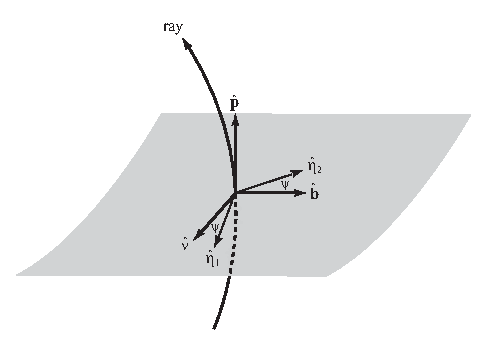
\includegraphics{../figures/chap15/fig03.eps}
\end{center}
\caption[shear wave basis]
{\label{15.fig.Spol}
Relation of the shear-wave polarization vectors
$\hat{\mbox{\boldmath $\eta$}}_1$ and
$\hat{\mbox{\boldmath $\eta$}}_2$ to
the ray normal $\hat{\mbox{\boldmath $\nu$}}$
and binormal $\hat{\bf b}$.
The shaded plane is perpendicular to the ray tangent~$\hat{\bf p}$;
the four vectors $\hat{\mbox{\boldmath $\nu$}}$, $\hat{\bf b}$
and $\hat{\mbox{\boldmath $\eta$}}_1$,
$\hat{\mbox{\boldmath $\eta$}}_2$
lie within this local wavefront plane.}
\end{figure}
The three vectors $\hat{\bp}$, $\betah_1$, $\betah_2$
form a right-handed orthonormal coordinate system:
$\hat{\bp}\cdot(\betah_1\times\betah_2)=1$.
Upon differentiating equations~(\ref{15.Sbasis}) and invoking
the Serret-Fr\'{e}net formulae~(\ref{15.Frenet}),
we find that
\eq \label{15.Sbasis2}
\frac{d\betah_1}{ds}=-\kappa\cos\psi\,\hat{\bp}
+(\tau+d\psi/\hspace{-0.3 mm}ds)\betah_2,
\en
\eq \label{15.Sbasis3}
\frac{d\betah_2}{ds}=\kappa\sin\psi\,\hat{\bp}
-(\tau+d\psi/\hspace{-0.3 mm}ds)\betah_1,
\en
where $\kappa$ and $\tau$ are the ray curvature and torsion,
respectively.  We see that we may render $d\betah_1/\hspace{-0.3 mm}ds$
and $d\betah_2/\hspace{-0.3 mm}ds$ parallel to $\bp$,
as required, by setting
\eq \label{15.Sbasis4}
\frac{d\psi}{ds}=-\tau.
\en
At the source point $\bx'$, we are free to choose the two
initial shear-wave polarizations $\betah^{\prime}_1=
\bnuh'\cos\psi'+\hat{\bb}^{\raisebox{-0.4 ex}
{$\scriptstyle\prime$}}\sin\psi'$ and $\betah^{\prime}_2
=-\bnuh'\sin\psi'+\hat{\bb}^{\raisebox{-0.4 ex}
{$\scriptstyle\prime$}}\cos\psi'$ arbitrarily.
The subsequent evolution of these independent
vectors along a ray is then given by
\eq \label{15.Sbasis5}
\betah_1=\betah^{\prime}_1-\int_0^s\kappa\cos\psi\,\hat{\bp}\,ds,
\qquad \betah_2=\betah^{\prime}_2+\int_0^s\kappa\sin\psi\,\hat{\bp}\,ds,
\en
where
\eq \label{15.Sbasis6}
\qquad\qquad\qquad\psi=\psi'-\int_0^s\tau\,ds.
\en
The basis vectors $\betah_1$ and $\betah_2$ twist around a \vspace{-0.4 mm}
ray relative to the normal $\bnuh$ and the binormal $\hat{\bb}$
at a rate~(\ref{15.Sbasis4}) that is {\em equal and opposite\/}
to the rate at which those vectors twist themselves.
In this sense, a shear wave in a laterally heterogeneous
Earth may be said to ``carry'' its
polarization with it as it propagates.
\index{shear-wave basis|)}%
\index{basis!shear-wave|)}%
\index{polarization!body-wave|)}%
\index{body-wave polarization|)}%

\renewcommand{\thesection}{$\!\!\!\raise1.3ex\hbox{$\star$}\!\!$
\arabic{chapter}.\arabic{section}}
\section{Effect of Boundaries}
\renewcommand{\thesection}{\arabic{chapter}.\arabic{section}}

Thus far our discussion of kinematic and dynamic ray tracing
has been limited to the smooth sub-region of the Earth surrounding
the source position.  In this section we consider the effect
of the external and internal boundaries $\Sigma=\p\earth\cup
\Sigma_{\rm SS}\cup\Sigma_{\rm FS}$.

\renewcommand{\thesubsection}{$\!\!\!\raise1.3ex\hbox{$\star$}\!\!$
\arabic{chapter}.\arabic{section}.\arabic{subsection}}
\subsection{Snell's law}
\index{Snell's law|(}%
\renewcommand{\thesubsection}{\arabic{chapter}.\arabic{section}.\arabic{subsection}}

The kinematic boundary conditions governing the
displacement~(\ref{15.JWKB}) require that the travel
time along a ray must be continuous:
\eq \label{15.Tcont}
[T]^+_-=0.
\en
It follows from~(\ref{15.Tcont}) that $[\bdel^{\Sigma}T]^+_-
=[\bdel T-\hat{\bn}\hspace{0.2 mm}\p_nT]^+_-=\bzero$.  Written in terms of
the slowness $\bp$, this condition takes the form
\eq \label{15.Snell}
[\bp^{\Sigma}]^+_-=[\bp-\bnh(\bnh\cdot\bp)]^+_-=\bzero.
\en
This is {\em Snell's law\/}---the tangential component
of the slowness must be continuous.  The jump discontinuity
in the normal component $[\bnh\cdot\bp]^+_-$ is determined
by this law, together with the condition that the Hamiltonian
must vanish on both sides of the boundary:
\eq \label{15.contHam}
[H]^+_-=\half[\bp\cdot\bp-v^{-2}]^+_-=0.
\en
The outgoing wave in equations~(\ref{15.Snell})--(\ref{15.contHam}) need not be
of the same type as the incident wave; furthermore, both conditions
pertain to reflected as well as transmitted waves, with an obvious
re-interpretation of the ``jump'' symbol $[\,\cdot\,]^+_-$.  In the
case of a P-to-P or S-to-S reflection, the normal component of the slowness
is reversed: $\bnh\cdot\bp\rightarrow -\bnh\cdot\bp$.
Hamilton's equations~(\ref{15.Hameqn}) in the smooth sub-regions of the Earth,
together with~(\ref{15.Snell})--(\ref{15.contHam}) on the boundaries
$\Sigma$, enable us to find $\bx$ and $\bp$, and thus the travel
time $T$, everywhere along a ray.
\index{Snell's law|)}%

\renewcommand{\thesubsection}{$\!\!\!\raise1.3ex\hbox{$\star$}\!\!$
\arabic{chapter}.\arabic{section}.\arabic{subsection}}
\subsection{Jump in geometrical spreading}
\index{geometrical spreading!jump in|(}%
\renewcommand{\thesubsection}{\arabic{chapter}.\arabic{section}.\arabic{subsection}}

The cross-sectional area of a ray tube $d\/\Sigma$,
and therefore the geometrical spreading
factor $\sR$, suffer jump discontinuities
at a boundary.  To calculate $[\sR]^+_-$ we must find the jumps in the
paraxial vectors $[\p_{\gamma^{\prime}}\bx]^+_-$ and $[\p_{\gamma^{\prime}}
\bp]^+_-$.  We consider a specific geometry for concreteness---an incoming
wave impinging upon the boundary $\Sigma$ from below, giving rise to a
transmitted wave in the overlying medium.  We seek to determine
the outgoing spreading factor given the incoming one:
$\sR_-\rightarrow\sR_+$.  The other transmitted case,
$\sR_+\rightarrow\sR_-$, and the two reflected cases,
$\sR_-\rightarrow\sR_-$ and $\sR_+\rightarrow\sR_+$,
require only a trivial modification.

The situation under consideration
is depicted in Figure~\ref{15.fig.boundary};
the central and paraxial rays strike the boundary at different points
$\bx$ and $\bx+d\bx_-$ and different ``instants'' $\sigma$ and
$\sigma+d\sigma_-$, as shown.
\begin{figure}[!b]
\begin{center}
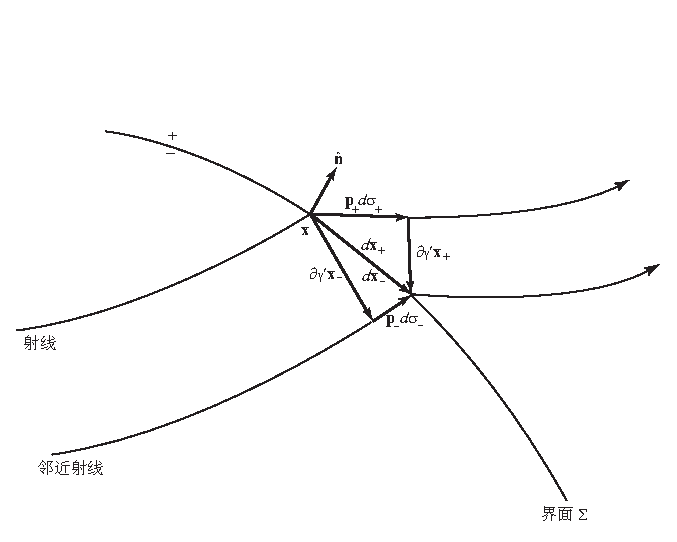
\includegraphics{../figures/chap15/fig04.eps}
\end{center}
\caption[boundary ray]
{\label{15.fig.boundary}
Schematic depiction of a ray tube impinging upon a boundary
from below.  The central ray and neighboring ray
intersect $\Sigma$ at the points ${\bf x}$ and ${\bf x}
+d{\bf x}$, respectively.  The unit normal to the
boundary at the point ${\bf x}$ is $\hat{\bf n}$.
The top-side and bottom-side differential vectors
$\partial_{\gamma'}{\bf x}_{\pm}$ both lie within
the wavefront.}
\end{figure}
We denote the slowness of the
incident ray at $\bx$ by
$\bp_{\raisebox{0.2 ex}{$\scriptstyle -$}}$, and the position and slowness
of the paraxial ray at the ``instant'' $\sigma$ by
$\bx+\p_{\gamma^{\prime}}\bx_-$ and
$\bp_{\raisebox{0.2 ex}{$\scriptstyle -$}}+
\p_{\gamma^{\prime}}\bp_{\raisebox{0.2 ex}{$\scriptstyle -$}}$.
The incident slowness at the paraxial intersection point $\bx+d\bx_-$
will be denoted by $\bp_{\raisebox{0.2 ex}{$\scriptstyle -$}}
+d\bp_{\raisebox{0.2 ex}{$\scriptstyle -$}}$.  We can relate the differential
intersection vectors $d\bx_-$,
$d\bp_{\raisebox{0.2 ex}{$\scriptstyle -$}}$ to the incoming vectors
$\p_{\gamma^{\prime}}\bx_-$,
$\p_{\gamma^{\prime}}\bp_{\raisebox{0.2 ex}{$\scriptstyle -$}}$
by first-order integration of Hamilton's equations~(\ref{15.Hameqn})
in the underlying medium:
\eq \label{15.farra1}
d\bx_-=\p_{\gamma^{\prime}}\bx_-+\p_{\subp}H_-\,d\sigma_-
=\p_{\gamma^{\prime}}\bx_-+
\bp_{\raisebox{0.2 ex}{$\scriptstyle -$}}\,d\sigma_-,
\en
\eq \label{15.farra2}
d\bp_{\raisebox{0.2 ex}{$\scriptstyle -$}}=
\p_{\gamma^{\prime}}\bp_{\raisebox{0.2 ex}{$\scriptstyle -$}}
-\p_{\subx}H_-\,d\sigma_-
=\p_{\gamma^{\prime}}\bp_{\raisebox{0.2 ex}{$\scriptstyle -$}}+
\half\bdel v_{\raisebox{0.4 ex}{$\scriptstyle -$}}^{-2}\,d\sigma_-.
\en
The propagation increment $d\sigma_-$ is determined by the first-order
condition $\bnh\cdot d\bx_-=0$ that both intersection points
lie upon the boundary:
\eq \label{15.farra3}
d\sigma_-=-\frac{\bnh\cdot\p_{\gamma^{\prime}}\bx_-}
{\bnh\cdot\bp_{\raisebox{0.2 ex}{$\scriptstyle -$}}}.
\en
Upon inserting equation~(\ref{15.farra3})
into~(\ref{15.farra1})--(\ref{15.farra2})
we obtain
\eq \label{15.farra4}
\left(\!\begin{array}{c}
d\bx_- \\ \vspace{-2.0 mm} \\ d\bp_{\raisebox{0.2 ex}{$\scriptstyle -$}}
\end{array}\!\right)=\left(\begin{array}{cc}
\bPi_{1-}  & \bzero  \\
\vspace{-2.0 mm}  & \\
\bPi_{2-}  & \bI
\end{array}\right)\cdot\left(\!\begin{array}{c}
\p_{\gamma^{\prime}}\bx_- \\
\vspace{-2.0 mm} \\
\p_{\gamma^{\prime}}\bp_{\raisebox{0.2 ex}{$\scriptstyle -$}}
\end{array}\!\right),
\en
where
\eq \label{15.farra5}
\bPi_{1-}=\bI-\frac{\bp_-\bnh}
{\bnh\cdot\bp_{\raisebox{0.2 ex}{$\scriptstyle -$}}},\qquad
\bPi_{2-}=-\half\frac{\bdel v_{\raisebox{0.4 ex}{$\scriptstyle -$}}^{-2}\bnh}
{\bnh\cdot\bp_{\raisebox{0.2 ex}{$\scriptstyle -$}}}.
\en
For convenience in what follows, we also
write~(\ref{15.farra4})--(\ref{15.farra5})
using an obvious six-vector notation:
$d\by_-=\bPi_-\cdot\p_{\gamma^{\prime}}\by_-$.

The central ray leaves the boundary from position
$\bx$ with slowness $\bp_{\raisebox{0.2 ex}{$\scriptstyle +$}}$;
we denote the departure
position and outgoing slowness of the paraxial ray by
$\bx+d\bx_+$ and $\bp_++d\bp_{\raisebox{0.2 ex}{$\scriptstyle +$}}$. 
Our next task is to
relate the differential vectors $d\bx_+$
and $d\bp_{\raisebox{0.2 ex}{$\scriptstyle +$}}$ to
$d\bx_-$ and $d\bp_{\raisebox{0.2 ex}{$\scriptstyle -$}}$.
Since both the central and
neighboring ray must be continuous,
the constraint upon the paraxial position is simple:
\eq  \label{15.farra6}
[d\bx]^+_-=\bzero.
\en
To find the jump in paraxial slowness $[d\bp]^+_-$,
we must account not only for the contrast in wave speed,
but also for the curvature of the boundary.
Perturbation of the continuity
conditions~(\ref{15.Snell})--(\ref{15.contHam})
leads to two constraints. Resolving the perturbations \vspace{-0.5 mm}
$d\bp_{\pm}=\bnh(\bnh\cdot d\bp_{\pm})+d\bp^{\Sigma}_{\pm}$
and noting that the unit normal at $\bx+d\bx_{\pm}$ is
$\bnh+d\bx_{\pm}\cdot\bdel^{\Sigma}\bnh$, we obtain
\eq \label{15.farra7}
[d\bp^{\Sigma}-(\bnh\cdot\bp)(d\bx\cdot\bdel^{\Sigma}\bnh)]^+_-=\bzero,
\en
\eqa \label{15.farra8} \lefteqn{
[dH]^+_-=[d\bx\cdot\p_{\subx}H+d\bp\cdot\p_{\subp}H]^+_-} \nonumber \\
&&\mbox{}\hspace{2.3 mm}
=[-\half\,d\bx\cdot\bdel v^{-2}+d\bp\cdot\bp]^+_-=0.
\ena
We have made use of the tangent character of the surface
curvature tensor, $\bnh\cdot\bdel^{\Sigma}\bnh=\bdel^{\Sigma}
\bnh\cdot\bnh=\bzero$, in deriving the pariaxial version
of Snell's law~(\ref{15.farra7}).  Equation~(\ref{15.farra8})
can be regarded as the boundary analogue of the smooth-medium
continuity condition~(\ref{15.dxdpeqn}).  A moderate amount
of straightforward algebra is required to manipulate these
two constraints into the desired form:
\eq \label{15.farra9}
\left(\!\begin{array}{c}
d\bx_+ \\ \vspace{-2.0 mm} \\ d\bp_{\raisebox{0.2 ex}{$\scriptstyle +$}}
\end{array}\!\right)=\left(\begin{array}{cc}
\bI  & \bzero  \\
\vspace{-2.0 mm}  & \\
\bT_1  & \bT_2
\end{array}\right)\cdot\left(\!\begin{array}{c}
d\bx_- \\ \vspace{-2.0 mm} \\ d\bp_{\raisebox{0.2 ex}{$\scriptstyle -$}}
\end{array}\!\right),
\en
where
\eqa \label{15.farra10} \lefteqn{
\bT_1=\bnh\cdot (\bp_{\raisebox{0.2 ex}{$\scriptstyle +$}}
-\bp_{\raisebox{0.2 ex}{$\scriptstyle -$}})\,\bdel^{\Sigma}\bnh
-\left(1-\frac{\bnh\cdot
\bp_{\raisebox{0.2 ex}{$\scriptstyle -$}}}
{\bnh\cdot\bp_{\raisebox{0.2 ex}{$\scriptstyle +$}}}\right)
\,\bnh\hspace{0.3 mm}\bp_{\raisebox{0.2 ex}
{$\scriptstyle +$}}\cdot\bdel^{\Sigma}\bnh} \nonumber \\
&&\mbox{}+\half\left(
\frac{1}{\bnh\cdot\bp_{\raisebox{0.2 ex}{$\scriptstyle +$}}}
\right)\bnh\bdel(v_{\raisebox{0.2 ex}{$\scriptstyle +$}}^{-2}
-v_{\raisebox{0.2 ex}{$\scriptstyle -$}}^{-2}),
\ena
\eq \label{15.farra11}
\bT_2=\bI-\bnh\bnh+\left(\frac{\bnh\cdot\bp_{\raisebox{0.2 ex}
{$\scriptstyle -$}}}
{\bnh\cdot\bp_{\raisebox{0.2 ex}{$\scriptstyle +$}}}\right)\bnh\bnh.
\en
The six-vector abbreviated form of~(\ref{15.farra10})--(\ref{15.farra11})
is $d\by_+=\bT\cdot d\by_-$.

Thus far we have followed the treatment
by Farra, Virieux \& Madariaga (\citeyear{farra&al89}).
We now take an additional step, and
extrapolate the top-side vectors $d\bx_+$ and
$d\bp_{\raisebox{0.2 ex}{$\scriptstyle +$}}$
in a manner
analogous to~(\ref{15.farra1})--(\ref{15.farra2})
to find new paraxial vectors $\p_{\gamma^{\prime}}\bx_+$ and
$\p_{\gamma^{\prime}}\bp_{\raisebox{0.2 ex}{$\scriptstyle +$}}$
in the overlying medium:
\eq \label{15.farra12}
d\bx_+=\p_{\gamma^{\prime}}\bx_++\p_{\subp}H_+\,d\sigma_+
=\p_{\gamma^{\prime}}\bx_+
+\bp_{\raisebox{0.2 ex}{$\scriptstyle +$}}\,d\sigma_+,
\en
\eq \label{15.farra13}
d\bp_{\raisebox{0.2 ex}{$\scriptstyle +$}}=
\p_{\gamma^{\prime}}\bp_{\raisebox{0.2 ex}{$\scriptstyle +$}}
-\p_{\subx}H_+\,d\sigma_+
=\p_{\gamma^{\prime}}\bp_{\raisebox{0.2 ex}{$\scriptstyle +$}}
+\half\bdel v_{\raisebox{0.4 ex}{$\scriptstyle +$}}^{-2}\,d\sigma_+.
\en
The outgoing increment $d\sigma_+$ can be determined by imposing the
constraint
$\bp_{\raisebox{0.2 ex}{$\scriptstyle +$}}\cdot\p_{\gamma^{\prime}}\bx_+=0$
that both
$\bx$ and $\bx+\p_{\gamma^{\prime}}\bx_+$ lie upon the same wavefront:
\eq \label{15.farra14}
d\sigma_+=\frac{\bp_{\raisebox{0.2 ex}{$\scriptstyle +$}}\cdot d\bx_+}
{\bp_{\raisebox{0.2 ex}{$\scriptstyle +$}}\cdot
\bp_{\raisebox{0.2 ex}{$\scriptstyle +$}}}.
\en
Upon inserting~(\ref{15.farra14}) into~(\ref{15.farra12})--(\ref{15.farra13})
we obtain
\eq \label{15.farra15}
\left(\!\begin{array}{c}
\p_{\gamma^{\prime}}\bx_+ \\
\vspace{-2.0 mm} \\
\p_{\gamma^{\prime}}\bp_{\raisebox{0.2 ex}{$\scriptstyle +$}}
\end{array}\!\right)=\left(\begin{array}{cc}
\bPi_{1+}  & \bzero  \\
\vspace{-2.0 mm}  & \\
\bPi_{2+}  & \bI
\end{array}\right)\cdot\left(\!\begin{array}{c}
d\bx_+ \\ \vspace{-2.0 mm} \\ d\bp_{\raisebox{0.2 ex}{$\scriptstyle +$}}
\end{array}\!\right),
\en
where
\eq \label{15.farra16}
\bPi_{1+}=\bI-\frac{\bp_+\bp_+}{\bp_+\cdot\bp_+},\qquad
\bPi_{2+}=-\half\frac{\bdel v_+^{-2}\bp_+}{\bp_+\cdot\bp_+}.
\en
We shall abbreviate this as $d\by_+=\bPi_+\cdot\p_{\gamma^{\prime}}\by_+$.

Upon concatenating the above results, we obtain the final relation
\eq \label{15.farra17}
\p_{\gamma^{\prime}}\by_+=\bB\cdot\p_{\gamma^{\prime}}\by_-\quad
\mbox{where}\quad\bB=\bPi_+\cdot\bT\cdot\bPi_-.
\en
Written out explicitly, equation~(\ref{15.farra17}) is
\eq \label{15.farra18}
\left(\!\begin{array}{c}
\p_{\gamma^{\prime}}\bx_+ \\
\vspace{-2.0 mm} \\
\p_{\gamma^{\prime}}\bp_{\raisebox{0.2 ex}{$\scriptstyle +$}}
\end{array}\!\right)=\left(\begin{array}{cc}
\bB_1  & \bzero  \\
\vspace{-2.0 mm}  & \\
\bB_2  & \bB_3
\end{array}\right)\cdot\left(\!\begin{array}{c}
\p_{\gamma^{\prime}}\bx_- \\
\vspace{-2.0 mm} \\
\p_{\gamma^{\prime}}\bp_{\raisebox{0.2 ex}{$\scriptstyle -$}}
\end{array}\!\right),
\en
where
\eq \label{15.farra19}
\bB_1=\bPi_{1+}\cdot\bPi_{1-},
\en
\eq
\bB_2=\bPi_{2+}\cdot\bPi_{1-}+\bT_1\cdot\bPi_{1-}
+\bT_2\cdot\bPi_{2-},
\en
\eq \label{15.farra20}
\bB_3=\bT_2.
\en
Equation~(\ref{15.farra18}) is
the relation needed to perform dynamical
ray tracing in the presence of boundaries.  We integrate
the linear system~(\ref{15.12eqns}) from the source point
$\bx'$ to the first boundary intersection,
use~(\ref{15.farra18}) to step from the $-$ side to the $+$
side, continue integrating to the next boundary, and so on.
Strictly speaking, the outgoing paraxial vectors
$\p_{\gamma^{\prime}}\bx_+$,
$\p_{\gamma^{\prime}}\bp_{\raisebox{0.2 ex}{$\scriptstyle +$}}$
are evaluated at $\sigma+d\sigma_-+d\sigma_+$ rather than
at $\sigma$; however, such a ``hiccup'' is inconsequential
in the limit of an infinitesimally narrow ray tube.
It should be noted that $\bB$ does {\em not\/} have the
requisite six degrees of freedom needed to be a full-fledged
boundary propagator, by virtue of the restriction
$\bp_{\raisebox{0.2 ex}{$\scriptstyle +$}}\cdot\p_{\gamma^{\prime}}\bx_+=0$.  For this reason,
it is not symplectic: $\bB^{\rm T}\cdot\bJ\cdot\bB\not=\bJ$.
\index{geometrical spreading!jump in|)}%

\renewcommand{\thesubsection}{$\!\!\!\raise1.3ex\hbox{$\star$}\!\!$
\arabic{chapter}.\arabic{section}.\arabic{subsection}}
\subsection{Polarization and energy partition}
\index{polarization!body-wave|(}%
\index{body-wave polarization|(}%
\index{reflection coefficient|(}%
\index{transmission coefficient|(}%
\renewcommand{\thesubsection}{\arabic{chapter}.\arabic{section}.\arabic{subsection}}

In addition to~(\ref{15.Tcont}) the JWKB ray sum at every
ray-boundary intersection point is required to satisfy
\eq \label{15.admiss1}
\sum_{\rm rays}\,[\bA]^+_-
=\bzero\quad\mbox{on $\Sigma_{\rm SS}$,}
\qquad \sum_{\rm rays}\,[\bnh\cdot\bA]^+_-
=0\quad\mbox{on $\Sigma_{\rm FS}$,}
\en
\eq \label{15.admiss2}
\sum_{\rm rays}\,[\bnh\cdot(\rho v A^2\hat{\bp})]^+_-=0\quad
\mbox{on all of $\Sigma$.}
\en
The first two relations~(\ref{15.admiss1}) are obvious kinematic
continuity conditions; the third~(\ref{15.admiss2}) is the dynamical
energy-flux conservation law~(\ref{15.couple}).  The sums
are over the incident ray and all of the reflected and
transmitted rays generated at the boundary.  The coupling
of incident and outgoing compressional and shear waves is
completely specified at every boundary point $\bx$ by
equations~(\ref{15.admiss1})--(\ref{15.admiss2}) together
with Snell's law~(\ref{15.Snell}).  Straightforward but
tedious algebra is all that is required to find the outgoing
wave amplitudes $\bA^{\rm out}$ in terms of the incident
amplitude $\bA^{\rm inc}$.  We do not give any details
here, but simply outline the essential physical ideas; for a
comprehensive treatment in ray-centered coordinates, see 
\v{C}erven\'{y}, Molotkov and P\v{s}en\v{c}\'{\i}k
(\citeyear{cerveny&al77}) or \v{C}erven\'{y}
(\citeyear{cerveny85}).

We begin by noting that it is possible to define local
``horizontal'' and ``vertical'' shear-wave polarizations
in terms of the unit slowness $\hat{\bp}$ of either the
incident or outgoing wave and the unit normal $\bnh$ at
every point on $\Sigma$:
\eq \label{15.locSHSV}
\betah_{\rm SH}=\pm\hspace{0.2 mm}\frac{\hat{\bp}\times\bnh}
{\|\hat{\bp}\times\bnh\|},\qquad
\betah_{\rm SV}=\pm(\betah_{\rm SH}\times\hat{\bp}),
\en
where the signs should be chosen to be consistent
with the spherical-Earth conventions summarized in
Figures~\ref{12.fig.polarization} and~\ref{12.fig.zhaoA1}.
Of course, the terminology ``horizontal'' and ``vertical''
and the designations SV and SH are something of a misnomer.
An incident P wave generates only outgoing P and SV waves,
just as in a spherically symmetric Earth.  The amplitudes
$A_{\rm P}^{\rm out}$ and $A_{\rm SV}^{\rm out}$ of these are
governed by the classical plane-wave $({\rm energy})^{1/2}$ reflection
and transmission coefficients, which we write using mnemonically
accented script-letter combinations such as $\acute{\sP}\grave{\sP}$,
$\acute{\sP}\hspace{-0.3 mm}\grave{\sS}$, $\acute{\sK}\grave{\sK}$
and $\acute{\sK}\acute{\sS}$ (see Section~\ref{12.sec.scatmat}).
The amplitude of the outgoing SH waves is $A_{\rm SH}^{\rm out}=0$.
An incident shear wave is more problematical since it
arrives with two independent polarizations $\betah_1^{\rm inc}$
and $\betah_2^{\rm inc}$ given by~(\ref{15.Sbasis}); normally,
these incoming polarizations will
not be aligned with $\betah_{\rm SV}$ and
$\betah_{\rm SH}$.  A general procedure which is suitable
for any kind of incoming wave consists of the following steps:
\begin{enumerate}
\item Find the orthogonal transformation $\ssQ^{\rm inc}$
that rotates the incoming slowness-polarization triad
$\hat{\bp}^{\rm inc}$, $\betah_1^{\rm inc}$, $\betah_2^{\rm inc}$
to $\hat{\bp}^{\rm inc}$, $\betah_{\rm SV}$, $\betah_{\rm SH}$.
\item Use the classical $({\rm energy})^{1/2}$ reflection and
transmission coefficients to calculate the amplitudes of all of
the outgoing P, SV and SH waves.
\item Find the orthogonal transformation $\ssQ^{\rm out}$ that
rotates every outgoing triad $\hat{\bp}^{\rm out}$,
$\betah_{\rm SV}$, $\betah_{\rm SH}$ to a new
$\hat{\bp}^{\rm out}$, $\betah_1^{\rm out}$, $\betah_2^{\rm out}$.
\end{enumerate}
The first and third steps are unnecessary for an incoming P wave.
The upshot of this procedure is
a $3\times 3$ forward scattering matrix
\eq \label{15.scatmat}
\ssS_+=\ssQ^{\rm out}\cdot\ssS^{\rm sub}_+\cdot\ssQ^{\rm inc}
\en
of {\em ray-specific\/} reflection and transmission
coefficients that relate the outgoing and incoming amplitudes
$A_{\rm P}^{\rm out}$, $A_{\rm S 1}^{\rm out}$,
$A_{\rm S 2}^{\rm out}$ and $A_{\rm P}^{\rm inc}$,
$A_{\rm S 1}^{\rm inc}$, $A_{\rm S 2}^{\rm inc}$.
Every compound ray between a source $\bx'$ and
receiver $\bx$ gives rise to a series of such
matrices, one at every boundary intersection
point along its path.  Reversal of all of the
rays likewise gives rise to a series of backward
scattering matrices of the form
\eq \label{15.scatmat2}
\ssS_-=(\ssQ^{\rm inc})^{\rm T}\cdot
\ssS^{\rm sub}_-\cdot(\ssQ^{\rm out})^{\rm T}.
\en
The interior sub-matrices $\ssS^{\rm sub}_{\pm}$
in~(\ref{15.scatmat})--(\ref{15.scatmat2})
are composed of the
appropriate elements of the full $6\times 6$
scattering matrices~(\ref{12.needin15});
for example, in the case of the bottom-side
reflections P{\scriptsize 660}P, P{\scriptsize 660}S,
S{\scriptsize 660}P, S{\scriptsize 660}S off
of the 660 km discontinuity,
\eq \label{15.scatmat3}
\ssS_{\pm}^{\rm sub}=\left(\hspace{1.5 mm}\begin{array}{ccc}
\acute{\sP}\grave{\sP} &
\hspace{-3.3 mm}\pm\acute{\sP}\hspace{-0.3 mm}\grave{\sS}
& \hspace{-2.0 mm}0 \\
\hspace{-2.3 mm}\pm\acute{\sS}\grave{\sP}
& \hspace{3.5 mm}\acute{\sS}\hspace{-0.1 mm}\grave{\sS}_{\rm SV}
& \hspace{-2.0 mm}0 \\
0 & 0 & \acute{\sS}\hspace{-0.1 mm}\grave{\sS}_{\rm SH}
\end{array}\right).
\en
The orthogonality
$(\ssQ^{\rm inc})^{\rm T}\cdot\ssQ^{\rm inc}=
(\ssQ^{\rm out})^{\rm T}\cdot\ssQ^{\rm out}=\ssI$
of the incident and outgoing coordinate transformations
and the $6\times 6$ ray-reversal symmetry relation~(\ref{12.scatsym})
guarantee that every pair of forward and backward
matrices~(\ref{15.scatmat})--(\ref{15.scatmat2}) satisfies
\eq \label{15.scatsym}
\ssS_-=\ssS_+^{\rm T},\qquad\ssS_+=\ssS_-^{\rm T}.
\en
The outgoing shear-wave polarizations may
be selected arbitrarily at every boundary encounter;
for example, it is possible simply to
set $\ssQ^{\rm out}=\ssI$, in which case
$\betah_1^{\rm out}=\betah_{\rm SV}$
and $\betah_2^{\rm out}=\betah_{\rm SH}$.  
The incoming polarizations $\betah_1^{\rm inc}$
and $\betah_2^{\rm inc}$ at the next boundary
can be found by an obvious modification of
equations~(\ref{15.Sbasis5})--(\ref{15.Sbasis6}).
The freedom to choose
$\betah_1^{\rm out}$ and $\betah_1^{\rm out}$
at each boundary is reminiscent of the freedom to
choose the initial polarizations $\betah^{\prime}_1$
and $\betah^{\prime}_2$ at the source.
\index{polarization!body-wave|)}%
\index{body-wave polarization|)}%
\index{reflection coefficient|)}%
\index{transmission coefficient|)}%

\section{Ray-Theoretical Response}
\index{response!body-wave|(}%
\index{body-wave response|(}%

We have at last collected all of the ingredients needed
to specify the ray-theoretical response.  We first find
the frequency-domain Green tensor $\bG(\bx,\bx';\om)$,
and then use it to determine the frequency-domain and
time-domain response to a moment-tensor source in
Section~\ref{15.sec.momresp}

\subsection{Green tensor}
\index{Green tensor!body-wave|(}%
\index{tensor!Green!body-wave|(}%

Ignoring boundary interactions and multi-pathing for the
moment, let us suppose that only a single
compressional-wave ray and two shear-wave rays
leave the source $\bx'$ and arrive at the receiver $\bx$.
We may write the JWKB Green tensor or impulse response
$\bG(\bx,\bx';\om)$ as a sum over these three rays:
\eq \label{15.Green1}
\bG=\frac{1}{4\pi}\sum_{\rm rays}
\betah\betah^{\raise-.1ex\hbox{$\scriptstyle\prime$}}
A'(\rho v)^{-1/2}\sR^{-1}\exp(-i\om T).
\en
The quantities $\betah'$ and $\betah$ are the
polarization vectors at the source and receiver,
respectively.  The compressional-wave polarization
is everywhere in the direction of propagation,
\eq \label{15.Green2}
\betah^{\prime}_{\rm P}=\hat{\bp}^{\prime}_{\rm P},\qquad
\betah_{\rm P}=\hat{\bp}_{\rm P},
\en
whereas the shear-wave polarizations at $\bx'$
and $\bx$ are connected by equations~(\ref{15.Sbasis5})--(\ref{15.Sbasis6}).
The geometrical-spreading term $(\rho v)^{-1/2}\sR^{-1}$
accounts for the variations in amplitude along the three
rays, in accordance with the energy-conservation
law~(\ref{15.amplaw}) and the definition~(\ref{15.sRdef}).
The initial amplitudes $A^{\prime}$ of the outgoing waves
remain to be determined.

We find these outgoing amplitudes by matching~(\ref{15.Green1})
to the far-field Green tensor of an infinite homogeneous medium in the
vicinity of the source; this classical far-field impulse response
$\bG_{\rm hom}(\bx,\bx';\omega)$
is given in terms of the source-receiver distance
$R=\|\bx-\bx'\|$ by (Aki \& Richards \citeyear{aki&richards80};
Ben-Menahem \& Singh \citeyear{ben-menahem&singh81})
\eq \label{15.Green3}
\bG_{\rm hom}=\frac{1}{4\pi}\sum_{\rm rays}
\betah^{\raise-.1ex\hbox{$\scriptstyle\prime$}}
\betah^{\raise-.1ex\hbox{$\scriptstyle\prime$}}
(\rho^{\prime}v^{\prime 2}R)^{-1}\exp(-i\om R/v').
\en
Noting that $\betah\rightarrow\betah^{\raise-.1ex\hbox{$\scriptstyle\prime$}}$,
$\rho\rightarrow\rho'$, $v\rightarrow v'$, $\sR\rightarrow R$
and $T\rightarrow R/v'$ in the near-source limit $\bx\rightarrow\bx'$,
we find that $A'=(\rho'v^{\prime 3})^{-1/2}$.  The Green
tensor~(\ref{15.Green1}) of a slightly heterogeneous infinite
medium is therefore
\eq \label{15.Green4}
\bG=\frac{1}{4\pi}\sum_{\rm rays}
\betah\betah^{\raise-.1ex\hbox{$\scriptstyle\prime$}}
(\rho\rho'vv^{\prime 3})^{-1/2}\sR^{-1}\exp(-i\om T).
\en
Three modifications are needed to generalize the result~(\ref{15.Green4})
so that it is valid for an Earth composed of several smooth
heterogeneous sub-regions $\earth=\earth_{\rm S}\cup\earth_{\rm F}$
separated by smooth boundaries $\Sigma=\p\earth
\cup\Sigma_{\rm SS}\cup\Sigma_{\rm FS}$.  First, we must sum over all
of the rays between the source $\bx'$ and the receiver $\bx'$,
including triplications and other multi-pathed arrivals as well
as boundary reflections and conversions.  Second, multi-pathing
implies the presence of caustics, and we must incorporate the
non-geometrical $\pi/2$ phase shifts that result from the changes
in sign of the ray-tube area.
Third, and finally, we must account for the
partition of energy associated with the proliferation of rays at
the boundaries.  The complete JWKB Green tensor has the same
form~(\ref{12.PGREEN}) as on a spherical Earth:
\eq \label{15.Green5}
\bG=\frac{1}{4\pi}\sum_{\rm rays}
\betah\betah^{\raise-.1ex\hbox{$\scriptstyle\prime$}}
(\rho\rho'vv^{\prime 3})^{-1/2}\Pi\sR^{-1}\exp(-i\om T
+iM\pi/2),
\en
where $M$ is the Maslov index, and $\Pi$ is the appropriate
product of ray-specific $({\rm energy})^{1/2}$ reflection
and transmission coefficients~(\ref{15.scatmat}).
The polarization vectors are interchanged and reversed,
$\betah\rightarrow -\betah'$, $\betah'\rightarrow -\betah'$,
upon an interchange of the source and receiver,
$\bx\rightarrow\bx'$, $\bx'\rightarrow\bx$.
\index{reciprocity!body waves}%
The seismic reciprocity relation
\eq \label{15.Green6}
\bG(\bx,\bx';\om)=\bG^{\rm T}(\bx',\bx;\om)
\en
is guaranteed by the kinematic equivalence
of the forward and reversed travel time,
$T(\bx,\bx')=T(\bx',\bx)$, together with
the dynamical spreading-factor, Maslov-index
and scattering-matrix symmetries~(\ref{15.Backus8}),
(\ref{15.Mrecip}) and~(\ref{15.scatsym}).
The initial shear-wave polarizations $\betah^{\prime}_1$,
$\betah^{\prime}_2$ are arbitrary along every
S ray leaving the source, as are the
polarizations $\betah^{\rm out}_1$,
$\betah^{\rm out}_2$ along every outgoing
S ray at every boundary.
The full ray-sum Green tensor~(\ref{15.Green5})
is, however, invariant with respect to these choices.
\index{tensor!Green!body-wave|)}%
\index{Green tensor!body-wave|)}%

\subsection{Moment-tensor response}
\index{moment-tensor response!body waves|(}%
\index{response!moment-tensor|(}%
\label{15.sec.momresp}

The ray-theoretical displacement response \vspace{-0.4 mm}
$s(\om)=\bnuh\cdot\bs(\bx,\omega)$
to a synchronous moment-tensor source
$\bM(\om)=\sqrt{2}M_0\hat{\bM}_{\,}m(\om)$ at a
hypocentral location $\bx_{\rm s}$ is also of the
same form~(\ref{12.DISP}) as on a spherical Earth:
\eq \label{15.DISP}
s(\om)=\frac{1}{4\pi}\sum_{\rm rays}\Xi\hspace{0.4 mm}\Sigma
\hspace{0.4 mm}\Pi\hspace{0.4 mm}\sR^{-1}
m(\om)\exp(-i\om T+iM\pi/\hspace{-0.2 mm}2),
\en
where
\eq \label{15.RECVR}
\Xi=(\rho v)^{-1/2}(\bnuh\cdot\betah),
\en
\eq \label{15.SOURC}
\Sigma=\sqrt{2}M_0(\rho_{\rm s}v_{\rm s}^5)^{-1/2}
[\hat{\bM}\!:\!\half(\hat{\bp}_{\rm s}\betah_{\rm s}
+\betah_{\rm s}\hat{\bp}_{\rm s})].
\en
The quantities $M_0$ and $\hat{\bM}$ are the scalar
moment and unit mechanism tensor of the earthquake,
and $m(\om)$ is the Fourier
transform of the normalized source time function
$\dot{m}(t)$.
The product $\hat{\bM}\!:\!\half(\hat{\bp}_{\rm s}
\betah_{\rm s} +\betah_{\rm s}\hat{\bp}_{\rm s})$ is the
radiation pattern of the waves upon leaving the source.  

The time-domain moment-tensor response obtained by inverse
Fourier transformation of equation~(\ref{15.DISP}) is
\eq \label{15.DISP2}
s(t)=\frac{1}{4\pi}\sum_{\rm rays}\Xi\hspace{0.4 mm}\Sigma
\hspace{0.4 mm}\Pi\hspace{0.4 mm}\sR^{-1}
\dot{m}_{\rm H}^{(M)}(t-T),
\en
where 
\eq
\dot{m}_{\rm H}^{(M)}(t)=\frac{1}{\pi}\,\Re{\rm e}
\int_0^{\infty}m(\om)\exp(i\om t+iM\pi/2)\,d\om.
\en
All $M=0$ waves travel along least-time ray paths, and
exhibit a far-field pulse shape $\dot{m}(t)$; every passage \vspace{-0.6 mm}
through a caustic gives rise to a Hilbert transformation:
$\dot{m}(t)\rightarrow\dot{m}_{\rm H}(t)\rightarrow\cdots
\rightarrow\dot{m}_{\rm H}^{\raisebox{-0.3 mm}{\scriptsize{(M)}}}(t)$.
Anelastic attenuation
and the associated physical dispersion can be accounted for by
convolution with an additional causal function, as in~(\ref{12.DISP3}):
\eq \label{15.DISP3}
s(t)=\frac{1}{4\pi}\sum_{\rm rays}\Xi\hspace{0.4 mm}\Sigma
\hspace{0.4 mm}\Pi\hspace{0.4 mm}\sR^{-1}
\dot{m}_{\rm H}^{(M)}(t-T)*a(t),
\en
where
\eq \label{15.atten}
a(t)=\frac{1}{\pi}\,\Re{\rm e}\int_0^{\infty}
\exp i\om\!\left[t+\half iT^{\ast}+\invpi T^{\ast}\ln
(\om\hspace{-0.2 mm}/\hspace{-0.2 mm}\om_0)\right]d\om.
\en
The attenuation time $T^{\ast}$ is given in terms of
\index{attenuation time}%
the wave speed $v_0$ at the reference frequency $\om_0$
and the anelastic quality factor $Q$ by the ray integral
\index{quality factor}%
\index{Q@{\em Q}}%
\eq \label{15.Tstar}
T^{\ast}=\int_{\subx^{\prime}}^{\subx}\frac{ds}{v_0Q}.
\en
\index{T@$T^{\ast}$}%
The quality factor $Q$ is $Q_\alpha$ along every compressional-wave leg
and $Q_\beta$ along every shear-wave leg of a ray.
The above results are valid provided that all of the
ray-specific reflection-and-transmission coefficients
in the product $\Pi$ are real.  Post-critical reflections
can be synthesized using a straightforward generalization
of the inverse Fourier transform~(\ref{15.DISP2}):
\eq \label{15.DISP4}
s(t)=\frac{1}{4\pi}\,\Re{\rm e}\sum_{\rm rays}\Xi\hspace{0.4 mm}\Sigma
\hspace{0.4 mm}\Pi\hspace{0.4 mm}\sR^{-1}
\dot{M}_{\rm H}^{(M)}(t-T)*a(t).
\en
The quantity $\dot{M}_{\rm H}^{(M)}(t)$ in~(\ref{15.DISP4})
is the $M$-times Hilbert transform of the {\em analytic\/}
source time function $\dot{M}(t)=\dot{m}(t)-i\dot{m}_{\rm H}(t)$.
\index{analytic source time function}%
\index{source time function!analytic}%

All of the above results break down in the vicinity of caustics,
where the cross-sectional area of a ray tube vanishes.  Uniformly
valid extensions of~(\ref{15.DISP4}) analogous to~(\ref{12.DISP4})
can be developed; such {\em Chapman-Maslov\/}
\index{Chapman-Maslov representation}%
representations express
the displacement $s(t)$ as either a one-dimensional or two-dimensional
integral over a family of rays $\gamma^{\prime}_1$, $\gamma^{\prime}_2$
leaving the source (Chapman \& Drummond \citeyear{chapman&drummond82};
Thomson \& Chapman \citeyear{thomson&chapman85};
Liu \& Tromp \citeyear{liu&tromp96}).   As a general rule,
the amplitude of seismic signal $s(t)$ is particularly strong or intense
in the vicinity of caustics, as might be expected from the
divergence $\sR^{-1}\rightarrow\infty$.  Indeed, the term caustic
comes from the Greek word $\kappa\alpha\upsilon\sigma
\tau\hspace{-0.2 mm}\acute{o}\sigma$ meaning ``burnt''.
\index{moment-tensor response!body waves|)}%
\index{response!body-wave|)}%
\index{body-wave response|)}%
\index{response!moment-tensor|)}%

\section{Practical Numerical Implementation}
\label{section:15.8}

We present a practical numerical scheme for calculating
synthetic ray-theoretical seismograms $s(t)$ in this section.
The seismic wave speed is presumed to be a specified function of
the form $v(r,\theta,\phi)$, where
$r$ is the radius, $\theta$ is the colatitude and $\phi$
is the longitude.  We restrict attention for simplicity to an
Earth with spherically symmetric external and internal boundaries
$\Sigma=\p\earth\cup\Sigma_{\rm SS}\cup\Sigma_{\rm FS}$; most
contemporary global three-dimensional models have this character
(Woodhouse \& Dziewonski \citeyear{woodhouse&dziewonski84};
Su, Woodward \& Dziewonski \citeyear{su&al94};
Masters, Johnson, Laske \& Bolton \citeyear{masters&al96};
Van der Hilst, Widiyantoro \& Engdahl \citeyear{vanderhilst&al96};
Dziewonski, Liu \& Su \citeyear{liu&dziewonski96}).

\subsection{Kinematic ray tracing}
\index{ray tracing!kinematic!body waves|(}%
\index{kinematic ray tracing!body waves|(}%
\label{15.sec.jeroen1}

We begin by expressing the slowness vector $\bp=\bdel T$ in terms of its
{\em covariant\/} spherical polar components:
\eq \label{15.LTpdef}
\bp=p_r\brh+r^{-1}p_\theta\,\bthetah
+(r\sin\theta)^{-1}p_\phi\,\bphih,
\en
where
\eq \label{15.LTcovar}
p_r=\p_rT,\qquad p_\theta=\p_\theta T,\qquad p_\phi=\p_\phi T.
\en
The eikonal equation~(\ref{15.Heqzero}) can be written in
terms of the position and conjugate momentum variables
$r,\theta,\phi$ and $p_r,p_{\theta},p_{\phi}$ in the form
\index{Hamiltonian!body-wave}%
\index{body-wave Hamiltonian}%
\eq \label{15.LTHam}
H=\half[p_r^2+r^{-2}p_\theta^2
+(r\sin\theta)^{-2}p_\phi^2-v^{-2}(r,\theta,\phi)]=0.
\en
Hamilton's equations for the Hamiltonian
$H(r,\theta,\phi,p_r,p_\theta,p_\phi)$ are
\eq
\frac{dr}{d\sigma}=\frac{\partial H}{\partial p_r}=p_r,
\label{15.LTdrdnu}
\en
\eq
\frac{d\theta}{d\sigma}=\frac{\partial H}{\partial p_\theta}
=r^{-2}p_\theta,
\en
\eq
\frac{d\phi}{d\sigma}=
\frac{\partial H}{\partial p_\phi}=(r\sin\theta)^{-2}p_\phi,
\label{15.LTdphidnu}
\en
\eq
\frac{dp_r}{d\sigma}=-\frac{\partial H}{\partial r}=\half\p_rv^{-2}
+r^{-3}[\hspace{0.3 mm}p_\theta^2+(\sin\theta)^{-2}p_\phi^2],
\en
\eq
\frac{dp_{\theta}}{d\sigma}=
-\frac{\partial H}{\partial\theta}=\half\p_\theta v^{-2}
+r^{-2}\cot\theta\,(\sin\theta)^{-2}p_\phi^2,
\en
\eq
\frac{dp_{\phi}}{d\sigma}
=-\frac{\partial H}{\partial\phi}=\half\p_\phi v^{-2}.
\label{15.LTdsphidnu}
\en
We seek solutions to~(\ref{15.LTdrdnu})--(\ref{15.LTdsphidnu})
subject to the six initial conditions
$r(0)=r'$, $\theta(0)=\theta'$, $\phi(0)=\phi'$ and
$p_r(0)=p^{\prime}_r$, $p_{\theta}(0)=p_{\theta}^{\prime}$,
$p_\phi(0)=p_{\phi}^{\prime}$.

We introduce the local {\em angle of incidence\/} $i$ and
\index{angle of incidence}%
\index{azimuth}%
{\em azimuth\/} $\zeta$ at every point $r,\theta,\phi$ along
a ray.  Following Aki \& Richards (\citeyear{aki&richards80}),
we measure $i$ downward from vertical and $\zeta$ counterclockwise
from due south, as illustrated in Figure~15.5.
\begin{figure}[!b]
\centering
\begin{tabular}{lr}
\begin{tabular}{l}
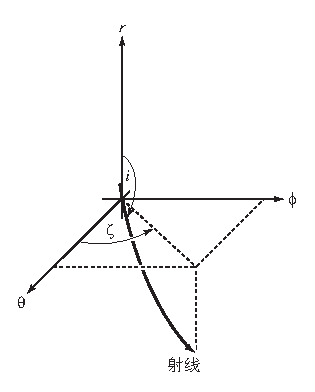
\includegraphics{../figures/chap15/fig05.eps}
\end{tabular}
&
\parbox{5.0cm}{\small
\vspace{0.05cm}
Figure~15.5. Schematic depiction of the local radial, colatitudinal
and longitudinal directions $r$, $\theta$, $\phi$ at
an arbitrary point along a ray.
The angle of incidence
$0\leq i\leq\pi$ is measured downward
from vertical, whereas the azimuth
$0\leq\zeta\leq 2\pi$ is measured counterclockwise
from due south.
The instantaneous direction of propagation is completely specified
by these two angles.}
\end{tabular}
\end{figure}
\addtocounter{figure}{1}
The slowness vector~(\ref{15.LTpdef}) can be written in terms of these
two ray-direction angles as
\eq
\bp=v^{-1}(\cos i\,\brh+\sin i\cos\zeta\,\bthetah+\sin i\sin\zeta\,\bphih).
\label{15.LTpdef2}
\en
The covariant components~(\ref{15.LTcovar}) of the slowness
\begin{displaymath}
p_r=v^{-1}\cos i,\qquad p_\theta=rv^{-1}\sin i\cos\zeta,
\end{displaymath}
\eq
\qquad\qquad
p_\phi=rv^{-1}\sin\theta\sin i\sin\zeta
\label{15.LTcovar2}
\en
are readily shown to satisfy the eikonal equation~(\ref{15.LTHam}).
We can use the relations~(\ref{15.LTcovar2}) to
transform~(\ref{15.LTdrdnu})--(\ref{15.LTdsphidnu})
into a system of first-order equations for $r$, $\theta$,
$\phi$ and $i$, $\zeta$:
\eq
\frac{dr}{d\sigma}=v^{-1}\cos i,
\label{15.LTray1}
\en
\eq
\frac{d\theta}{d\sigma}=r^{-1}v^{-1}\sin i\cos\zeta,
\en
\eq
\frac{d\phi}{d\sigma}=
r^{-1}v^{-1}(\sin\theta)^{-1}\sin i\sin\zeta,
\label{15.LTray3}
\en
\eqa \lefteqn{
\frac{di}{d\sigma}=
-\sin i\,(r^{-1}v^{-1}+\p_rv^{-1})}
\nonumber \\
&&\mbox{}\qquad\hspace{-1.85 mm}
+r^{-1}\cos i\,[\cos\zeta\,\p_\theta v^{-1}
+(\sin\theta)^{-1}\sin\zeta\,\p_\phi v^{-1}],
\ena
\eqa
\lefteqn{\frac{d\zeta}{d\sigma}=
-r^{-1}(\sin i)^{-1}\sin\zeta\,\p_\theta v^{-1}} \nonumber \\
&&\mbox{}\qquad\hspace{-1.3 mm}
+r^{-1}(\sin\theta)^{-1}(\sin i)^{-1}\cos\zeta\,\p_\phi v^{-1}
\nonumber \\
&&\mbox{}\qquad\hspace{-1.3 mm}-r^{-1}v^{-1}\cot\theta\sin i\sin\zeta.
\label{15.LTray5}
\ena
It is convenient to choose the two ray parameters to be
the outgoing incidence angle and azimuth at the source:
\eq \label{15.LTgamdef}
\gamma^{\prime}_1=i',\qquad\gamma^{\prime}_2=\zeta'.
\en
The initial conditions associated with the five
equations~(\ref{15.LTray1})--(\ref{15.LTray5}) are then
$r(0)=r'$, $\theta(0)=\theta'$, $\phi(0)=\phi'$ and
$i(0)=i'$, $\zeta(0)=\zeta'$.

We can reduce the above results
even further by taking the longitude $\phi$ to be
the independent variable.  Using~(\ref{15.LTray3})
to eliminate $\sigma$, we obtain a final system
of {\em four kinematic ray-tracing equations\/}:
\eq
\frac{dr}{d\phi}
=r\sin\theta\cot i\,(\sin\zeta)^{-1},
\label{15.LTeq1}
\en
\eq
\frac{d\theta}{d\phi}
=\sin\theta\cot\zeta,
\label{15.LTeq2}
\en
\eqa \lefteqn{
\frac{di}{d\phi}
=\sin\theta\,(\sin\zeta)^{-1}
(r\p_r\hspace{-0.4 mm}\ln v-1)} \nonumber \\
&&\mbox{}\qquad\hspace{-1.3 mm}
-\sin\theta\cot i\cot\zeta\,\p_\theta\hspace{-0.4 mm}\ln v
-\cot i\,\p_\phi\hspace{-0.4 mm}\ln v,
\label{15.LTeq3}
\ena
\eqa \lefteqn{
\frac{d\zeta}{d\phi}=-\cos\theta+
\sin\theta\,(\sin i)^{-2}\p_\theta\hspace{-0.4 mm}\ln v} \nonumber \\
&&\mbox{}\qquad\hspace{-1.3 mm}
-(\sin i)^{-2}\cot\zeta\,\p_\phi\hspace{-0.4 mm}\ln v.
\label{15.LTeq4}
\ena
At every spherically symmetric discontinuity, these differential
equations must be supplemented by the continuity conditions
\eq \label{15.LTbconds}
[r]^+_-=0,\qquad[\theta]^+_-=0,\qquad
[v^{-1}\sin i]^+_-=0,\qquad[\zeta]^+_-=0.
\en
\begin{figure}[!b]
\begin{center}
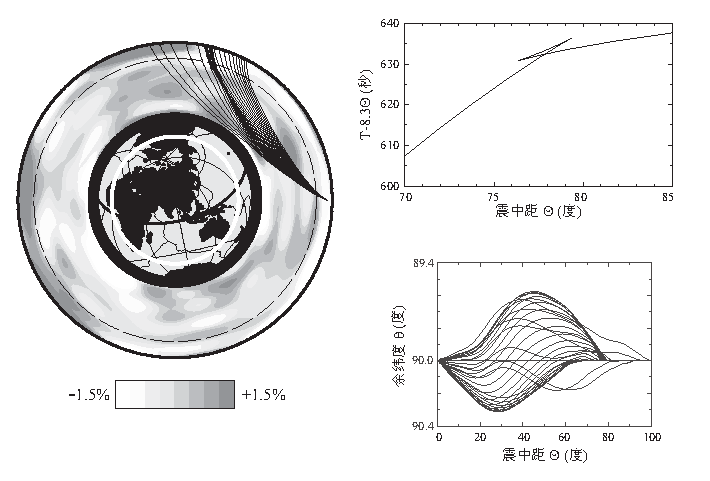
\includegraphics{../figures/chap15/fig06.eps}
\end{center}
\caption[liu&tromp Fig 2]
{\label{15.fig.LTfig2}
S-wave trajectories in the $s_{\rm max}=12$ Earth model SKS12WM13.
Rays are shot from a 200~km deep event in Fiji toward North America.
({\em Left\/}) White circle on interior map indicates the
great circle through the source and the family of receivers; this
circle is the equator in the rotated coordinate system used to trace
rays.  Outer cross-section shows mantle shear-wave speed perturbations
in the source-receiver plane; long-dashed circle is the 670~km discontinuity.
Scale bar shows the range $-1.5\%\leq \delta\hspace{-0.1 mm}\beta/\beta\leq
1.5\%$ of relative perturbations; darker-shaded regions have higher speeds.
All rays strike the surface of the Earth along
the rotated equator; curves show the projection of these rays onto the
cross-section.  ({\em Top right}) The reduced travel-time curve for these
perturbed equatorial rays exhibits a small-scale triplication;
the associated caustics
at $\Theta\approx 76.5^{\circ}$ and $\Theta\approx 79^{\circ}$ are apparent
in the cross-section.  ({\em Bottom right}) Rays projected
onto the Earth's surface; the ordinate $\theta$ is the rotated
colatitude.  The equatorial location of the receivers is evident
in this map view.}
\end{figure}
Prior to integrating~(\ref{15.LTeq1})--(\ref{15.LTbconds}),
it is advantageous to rotate the Earth model so that both
the source and receiver are situated on the equator
(see Appendix~\ref{section:C.8.7}):
\eq \label{15.eqrot}
\theta'=\pi/2,\;\phi'=0\quad\mbox{and}\quad
\theta=\pi/2,\;\phi=\Theta,
\en
where $\cos\Theta=\cos\theta\cos\theta'
+\sin\theta\sin\theta'\cos(\phi-\phi')$.
The initial conditions in that case are
\eq
r(0)=r',\qquad\theta(0)=\pi/2,
\qquad i(0)=i',\qquad\zeta(0)=\zeta'.
\label{15.LTb}
\en
Since the longitude $\phi$ always increases along a ray
in such an equatorial coordinate system, singularities
associated with due north-south propagation $\zeta=0,\pi$
do not arise.
\index{ray tracing!kinematic!body waves|)}%
\index{kinematic ray tracing!body waves|)}%

\subsection{Shooting}
\index{shooting!body waves|(}%
\index{ray shooting!body waves|(}%
\label{15.sec.2point}

The {\em two-point\/} ray-tracing problem requires us
\index{two-point ray tracing}%
\index{ray tracing!two-point}%
to find the initial takeoff angles $i'$, $\zeta'$ that
\index{takeoff angle}%
enable a ray to ``hit'' the receiver.  For a receiver
situated on the Earth's surface $r=a$, the endpoint
conditions are
\eq \label{15.LThitter}
r(\Theta)=a,\qquad\theta(\Theta)=\pi/2.
\en
A number of iterative schemes are available to solve
this {\em ray-shooting\/} problem
\index{shooting}%
(Julian \& Gubbins
\citeyear{julian&gubbins77}).  Whenever the geometrical spreading factor
$\sR$ must also be calculated, it is natural to use Newton's method;
dropping the argument $\Theta$ for simplicity we update $i'$ and
$\zeta'$ using
\eq \label{15.LTNewton}
\left(\!\begin{array}{cc}
\p_{i'}r_n  & \p_{\zeta'}r_n \\
\vspace{-2.0 mm} \\
\p_{i'}\theta_n  & \p_{\zeta'}\theta_n
\end{array}\!\right)\!
\left(\!\begin{array}{c}
i_{n+1}^{\prime}-i_n^{\prime} \\
\vspace{-2.0 mm} \\
\zeta_{n+1}^{\prime}-\zeta_n^{\prime}
\end{array}\!\right)=
\left(\!\begin{array}{c}
a-r_n \\
\vspace{-2.0 mm} \\
\pi/2-\theta_n
\end{array}\!\right),
\en
where $n=0,1,2,\ldots$ denotes the iteration number.
The required partial derivatives
$\p_{i'}r_n$, $\p_{\zeta'}r_n$ and $\p_{i'}\theta_n$,
$\p_{\zeta'}\theta_n$ are available as solutions to the
dynamical ray-tracing equations in Section~\ref{15.sec.jeroen2}.
Convergence is expedited by a good first guess $i^{\prime}_0$,
$\zeta^{\prime}_0$; perturbation theory provides such an initial
iterate, as we discuss in Section~15.9.3.
Several examples of S-wave rays traced through the three-dimensional
Earth model SKS12WM13 (Dziewonski, Liu \& Su \citeyear{liu&dziewonski96})
are shown in Figure~\ref{15.fig.LTfig2}.  Small-scale travel-time
triplications such as the one illustrated here are a ubiquitous
feature at epicentral distances beyond $\Theta=75^{\circ}$,
because of the strong lateral heterogeneity in the lowermost
mantle.  The third arrival of every such triplication has
passed through the associated caustic, whereas the first and
the second have not.  The rays in model SKS12WM13 wander no more
than $0.3^{\circ}\!\!-\!0.4^{\circ}$ out of the spherical-Earth
ray plane.
The trajectory of a typical SS ray is depicted
in Figure~\ref{15.fig.LTfig13}.  The minimax character
\index{minimax phase}%
\index{phase!minimax}%
of this phase is responsible for the pronounced ray-path
deviations; the surface bounce points may be displaced as
much as $2^{\circ}$ away from the corresponding point
in the spherical Earth.
\begin{figure}[!t]
\begin{center}
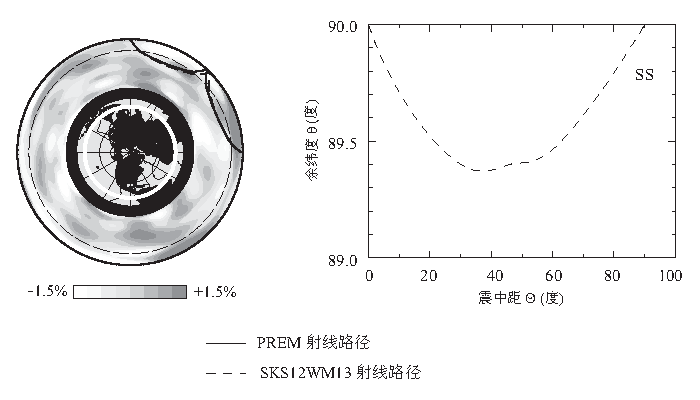
\includegraphics{../figures/chap15/fig07.eps}
\end{center}
\caption[liu&tromp Fig 13]
{\label{15.fig.LTfig13}
Comparison of an SS ray path in model SKS12WM13 and PREM.
The source is situated on the equator and Greenwich Meridian,
and the receiver is situated due east at an epicentral distance
$\Theta=90^{\circ}$.  The PREM surface bounce point is at
$\Theta/2=45^{\circ}$, in the vicinity of the East African Rift Valley.
({\em Left\/}) Unperturbed ({\em solid line\/}) and perturbed
({\em dashed line\/}) rays projected on a cross-section through model
SKS12WM13; see caption to Figure~\ref{15.fig.LTfig2} for explanation
of interior map and other plotting conventions.
({\em Right\/}) Projection of the two ray paths
onto the Earth's surface; the PREM ray is confined to the equatorial plane.
The out-of-plane deviations are approximately twice as large as those
of a typical teleseismic S wave.}
\end{figure}
\index{shooting!body waves|)}%
\index{ray shooting!body waves|)}%

\subsection{Travel time and attenuation time}
\index{travel time!body-wave|(}%
\index{body-wave travel time|(}%
\index{body-wave attenuation|(}%
\index{attenuation time|(}%
\index{T@$T^{\ast}$|(}%

The variation of the travel time along a ray can be found from the
differential relation $d\sigma=v^2dT$ together with equation~(\ref{15.LTray3}):
\eq
\frac{dT}{d\phi}=
rv^{-1}\sin\theta\,(\sin i\,\sin\zeta)^{-1}.
\label{15.LTtravtime}
\en
This can be integrated to find the total travel time
of any minor-arc body-wave phase in an elastic Earth:
\eq
T=\int_0^\Theta rv^{-1}\sin\theta\,(\sin i\,\sin\zeta)^{-1}\,d\phi.
\label{15.LTt}
\en
The attenuation time~(\ref{15.Tstar}) in an anelastic Earth is likewise
given by
\eq
T^\ast=\int_0^\Theta rv_0^{-1}Q^{-1}
\sin\theta\,(\sin i\,\sin\zeta)^{-1}\,d\phi,
\label{15.LTtstar}
\en
where $v_0$ is the wave speed---either $\alpha_0$
or $\beta_0$---at the reference frequency $\om_0$,
and $Q$ is the associated compressional-wave or
shear-wave quality factor $Q_{\alpha}$ or $Q_{\beta}$.
Equations~(\ref{15.LTt}) and~(\ref{15.LTtstar}) assume that the
source and receiver are both situated on the equator, as in~(\ref{15.eqrot}).
\index{travel time!body-wave|)}%
\index{body-wave travel time|)}%
\index{body-wave attenuation|)}%
\index{attenuation time|)}%
\index{T@$T^{\ast}$|)}%

\subsection{Geometrical spreading factor}
\index{geometrical spreading!body waves|(}%

The differential area of a ray tube~(\ref{15.Jacob3}) and the
solid angle subtended by that tube at the source are given
in terms of the initial takeoff angles $i'$ and $\zeta'$ by
\index{takeoff angle}%
\eq \label{15.LTtwod}
d\/\Sigma=vJ\,di'\,d\zeta',\qquad
d\/\Omega=\sin i'\,di'\,d\zeta'.
\en
The geometrical spreading factor $\sR=\sqrt{|d\/\Sigma|/d\/\Omega}$ is
therefore related to the Jacobian
\index{point-source Jacobian!body waves}%
\index{Jacobian!point-source!body waves}%
\eq \label{15.LTJdef}
J=\frac{\p(x_1,x_2,x_3)}{\p(\sigma,i',\zeta')}
={\rm det}\left(\begin{array}{ccc}
\displaystyle{\frac{\p x_1}{\p\sigma}} &
\displaystyle{\frac{\p x_1}{\p i'}} &
\displaystyle{\frac{\p x_1}{\p\zeta'}} \\
\vspace{-2.0 mm} && \\
\displaystyle{\frac{\p x_2}{\p\sigma}} &
\displaystyle{\frac{\p x_2}{\p i'}} &
\displaystyle{\frac{\p x_2}{\p\zeta'}} \\
\vspace{-2.0 mm} && \\
\displaystyle{\frac{\p x_3}{\p\sigma}} &
\displaystyle{\frac{\p x_3}{\p i'}} &
\displaystyle{\frac{\p x_3}{\p\zeta'}} \\
\end{array}\right)
\en
by $\sR=\sqrt{v|J|/\!\sin i'}$.
We can express $J$ in terms of the spherical polar coordinates
$r,\theta,\phi$ using the composition rule for coordinate transformations:
\eqa \label{15.LTdets} \lefteqn{
J=\frac{\p(x_1,x_2,x_3)}{\p(r,\theta,\phi)}\;
\frac{\p(r,\theta,\phi)}{\p(i',\zeta',\phi)}\;
\frac{\p(i',\zeta',\phi)}{\p(\sigma,i',\zeta')}} \nonumber \\
&&\mbox{}\hspace{-4.7 mm}
=rv^{-1}\sin i\sin\zeta\;\frac{\p(r,\theta)}{\p(i',\zeta')},
\ena
where we have evaluated the three determinants and made use
of~(\ref{15.LTray3}) in deducing the second equality.
The final spherical polar expression for the spreading
factor obtained in this way is
\index{geometrical spreading factor!body waves}%
\eq \label{15.LTRdef}
\sR=\sqrt{r\,(\sin i')^{-1}\sin i\sin\zeta\,|\Upsilon|},
\en
where we have introduced the two-dimensional spherical polar Jacobian
\eq
\Upsilon=\frac{\p(r,\theta)}{\p(i',\zeta')}
=\frac{\p r}{\p i'}\frac{\p\theta}{\p\zeta'}
-\frac{\p r}{\p\zeta'}\frac{\p\theta}{\p i'}.
\label{15.LTjacs}
\en
Only four partial derivatives need to be evaluated:
$\p_{i'}r$, $\p_{\zeta'}r$ and $\p_{i'}\theta$, $\p_{\zeta'}\theta$.
\index{geometrical spreading!body waves|)}%

\subsection{Dynamical ray tracing}
\index{dynamical ray tracing!body waves|(}%
\index{ray tracing!dynamical!body waves|(}%
\label{15.sec.jeroen2}

To compute these, we differentiate~(\ref{15.LTeq1})--(\ref{15.LTeq4})
with respect to the initial takeoff angles $i'$ and $\zeta'$.  This
yields a system of {\em eight dynamical ray-tracing equations\/}:
\eqa \label{15.LTpeq1}
\lefteqn{\frac{d}{d\phi}(\p_{\gamma'}r)
=\sin\theta\cot i\,(\sin\zeta)^{-1}\p_{\gamma'}r} \nonumber \\
&&\mbox{}+r\cos\theta\cot i\,(\sin\zeta)^{-1}\p_{\gamma'}\theta
\nonumber \\
&&\mbox{}-r\sin\theta\,(\sin i)^{-2}(\sin\zeta)^{-1}
\p_{\gamma'}i \\
&&\mbox{}-r\sin\theta\cot i\cot\zeta\,
(\sin\zeta)^{-1}\p_{\gamma'}\zeta, \nonumber
\ena
\eqa \label{15.LTpeq2} \lefteqn{
\frac{d}{d\phi}(\p_{\gamma'}\theta)
=\cos\theta\cot\zeta\,\p_{\gamma'}\theta
-\sin\theta\,(\sin\zeta)^{-2}\p_{\gamma'}\zeta,}
\ena
\eqa \label{15.LTpeq3}
\lefteqn{\frac{d}{d\phi}(\p_{\gamma'}i)
=[\sin\theta\,(\sin\zeta)^{-1}
(r\p_r^2\hspace{-0.2 mm}\ln v+\p_r\hspace{-0.4 mm}\ln v)} \nonumber \\
&&\mbox{}\qquad-\cot i\,(\sin\theta\cot\zeta\,
\p_r\p_{\theta}\hspace{-0.4 mm}\ln v
+\p_r\p_{\phi}\hspace{-0.4 mm}\ln v)]\,\p_{\gamma'}r \nonumber \\
&&\mbox{}+[\sin\theta\,(\sin\zeta)^{-1}r\p_r\p_{\theta}\hspace{-0.4 mm}\ln v
+\cos\theta\,(\sin\zeta)^{-1}(r\p_r\hspace{-0.4 mm}\ln v-1) \nonumber \\
&&\mbox{}\qquad-\cot i\,(\sin\theta\cot\zeta\,
\p^2_{\theta}\hspace{-0.2 mm}\ln v
+\p_{\theta}\p_{\phi}\hspace{-0.4 mm}\ln v \nonumber \\
&&\mbox{}\qquad
+\cos\theta\cot\zeta\,\p_{\theta}\hspace{-0.4 mm}\ln v)]\,\p_{\gamma'}\theta \\
&&\mbox{}+(\sin i)^{-2}(\sin\theta\cot\zeta\,
\p_\theta\hspace{-0.4 mm}\ln v+\p_\phi\hspace{-0.4 mm}\ln v)
\p_{\gamma'}i \nonumber \\
&&\mbox{}-\sin\theta\,(\sin\zeta)^{-2}[\cos\zeta\,
(r\p_r\hspace{-0.4 mm}\ln v-1)
-\cot i\,\p_{\theta}\hspace{-0.4 mm}\ln v]\,\p_{\gamma'}\zeta, \nonumber
\ena
\eqa \label{15.LTpeq4}
\lefteqn{\frac{d}{d\phi}(\p_{\gamma'}\zeta)=(\sin i)^{-2}
(\sin\theta\,\p_r\p_{\theta}\hspace{-0.4 mm}\ln v-
\cot\zeta\,\p_r\p_{\phi}\hspace{-0.4 mm}\ln v)\,\p_{\gamma'}r} \nonumber \\
&&\mbox{}+[(\sin i)^{-2}(\sin\theta\,\p^2_{\theta}\hspace{-0.2 mm}\ln v
-\cot\zeta\,\p_{\theta}\p_{\phi}\hspace{-0.4 mm}\ln v \nonumber \\
&&\mbox{}\qquad+\cos\theta\,\p_{\theta}\hspace{-0.4 mm}\ln v)+\sin\theta]
\,\p_{\gamma'}\theta \\
&&\mbox{}-2\cot i\,(\sin i)^{-2}(\sin\theta\,\p_{\theta}\hspace{-0.4 mm}\ln v
-\cot\zeta\,\p_{\phi}\hspace{-0.4 mm}\ln v)\,\p_{\gamma'}i \nonumber \\
&&\mbox{}+(\sin i)^{-2}(\sin\zeta)^{-2}(\p_\phi\hspace{-0.4 mm}\ln v)\,
\p_{\gamma'}\zeta, \nonumber
\ena
where $\gamma'$ denotes either $i'$ or $\zeta'$.  These
must be solved subject to the initial conditions
\begin{displaymath}
\p_{i'}r(0)=\p_{\zeta'}r(0)=0,\qquad
\p_{i'}\theta(0)=\p_{\zeta'}\theta(0)=0,
\end{displaymath}
\eq
\p_{i'}\zeta(0)=\p_{\zeta'}i(0)=0,\qquad
\p_{i'}i(0)=\p_{\zeta'}\zeta(0)=1.
\label{15.LTbpeq}
\en
The dependence upon the unknown partial derivatives
in~(\ref{15.LTpeq1})--(\ref{15.LTpeq4}) is linear,
and the equations governing $\p_{i'}r$, $\p_{i'}\theta$,
$\p_{i'}i$, $\p_{i'}\zeta$ are decoupled from those governing
$\p_{\zeta'}r$, $\p_{\zeta'}\theta$, $\p_{\zeta'}i$, $\p_{\zeta'}\zeta$,
as in the Cartesian dynamical ray-tracing system~(\ref{15.12eqns}).

At a discontinuity the differential
equations~(\ref{15.LTpeq1})--(\ref{15.LTpeq4})
must be supplemented by conditions analogous
to~(\ref{15.LTbconds}) that specify the jumps in the
eight derivatives $\p_{\gamma'}r$, $\p_{\gamma'}\theta$,
$\p_{\gamma'}i$ and $\p_{\gamma'}\zeta$.  Let us
denote the parameters of a central and neighboring ray
at the intersection points $\bx$ and $\bx+d\bx$ in
Figure~\ref{15.fig.boundary} by $r$,
$\theta$, $\phi$, $i$, $\zeta$ and $r+dr$,
$\theta+d\theta$, $\phi+d\phi$, $i+di$,
$\zeta+d\zeta$.  Since every point along
a ray is uniquely determined by the initial
takeoff angles $i'$, $\zeta'$ and the longitude
$\phi$, we can express $dr$
in terms of $di'$, $d\zeta'$ and $d\phi$ in the form
$dr=di'\,\p_{i'}r+d\zeta'\,\p_{\zeta'}r+d\phi\,\p_{\phi}r$.
At a spherical boundary we must have $dr=0$;
it follows that $d\phi=-(dr\hspace{-0.3 mm}/\hspace{-0.3 mm}d\phi)^{-1}
(di'\,\p_{i'}r+d\zeta'\,\p_{\zeta'}r)$,
where we have replaced $\p_{\phi}r$ by
$dr\hspace{-0.3 mm}/\hspace{-0.3 mm}d\phi$
in accordance with our usual convention.
The continuity condition $[d\phi]^+_-=0$ and
the independence of the perturbations $di'$
and $d\zeta'$ imply that the quantities
$(dr\hspace{-0.3 mm}/\hspace{-0.3 mm}d\phi)^{-1}\p_{i'}r$
and $(dr\hspace{-0.3 mm}/\hspace{-0.3 mm}d\phi)^{-1}\p_{\zeta'}r$
must both be continuous.  The perturbed versions $[d\theta]^+_-=0$,
$[-v^{-2}dv\sin i+v^{-1}di\cos i]^+_-=0$ and $[d\zeta]^+_-=0$
of the remaining continuity conditions~(\ref{15.LTbconds})
likewise constrain the jumps in the other partial derivatives.
The complete set of boundary conditions at every spherical
discontinuity is
\begin{displaymath}
[(dr\hspace{-0.3 mm}/\hspace{-0.3 mm}d\phi)^{-1}\p_{\gamma'}r]^+_-=0,\qquad
[\p_{\gamma'}\theta]^+_-=0,
\end{displaymath}
\vspace{-3.0 mm}
\eqa \lefteqn{
[\cot i\,\p_{\gamma'}i-(\p_{\theta}\hspace{-0.4 mm}\ln v)\,\p_{\gamma'}\theta
+(dr\hspace{-0.3 mm}/\hspace{-0.3 mm}d\phi)^{-1}}
\nonumber \\
&&\mbox{}\times\{(d\theta\hspace{-0.3 mm}
/\hspace{-0.3 mm}d\phi)\,\p_{\theta}\hspace{-0.4 mm}\ln v
+\p_{\phi}\hspace{-0.4 mm}\ln v-\cot i
\,(di\hspace{-0.3 mm}/\hspace{-0.3 mm}d\phi)\hspace{0.2 mm}\}
\,\p_{\gamma'}r]^+_-=0, \nonumber
\ena
\eq \label{15.LTlas}
[\p_{\gamma'}\zeta-
(dr\hspace{-0.3 mm}/\hspace{-0.3 mm}d\phi)^{-1}
(d\zeta\hspace{-0.3 mm}/\hspace{-0.3 mm}d\phi)
\p_{\gamma'}r]^+_-=0.
\en
In deriving~(\ref{15.LTlas}) we have used Snell's law
$[v^{-1}\sin i]^+_-=0$ in addition to the continuity condition
$[d\theta\hspace{-0.3 mm}/\hspace{-0.3 mm}d\phi]^+_-=0$.
\index{dynamical ray tracing!body waves|)}%
\index{ray tracing!dynamical!body waves|)}%

\renewcommand{\thesubsection}{$\!\!\!\raise1.3ex\hbox{$\star$}\!\!$
\arabic{chapter}.\arabic{section}.\arabic{subsection}}
\subsection{Maslov index}
\index{Maslov index!body waves|(}%
\index{index!Maslov|(}%
\renewcommand{\thesubsection}{\arabic{chapter}.\arabic{section}.\arabic{subsection}}

The ray-tube singularity conditions~(\ref{15.causfocdef}) may
be expressed in terms of spherical polar coordinates in the form
\eq \label{15.causfocdef2}
\begin{array}{ll}
\mbox{caustic:} & (\p_{i'}r)(\p_{\zeta'}\theta)
=(\p_{\zeta'}r)(\p_{i'}\theta)\not=0, \\
\vspace{-1.5 mm} & \vspace{-1.5 mm} \\
\mbox{focal~point:} & (\p_{i'}r)(\p_{\zeta'}\theta)
=(\p_{\zeta'}r)(\p_{i'}\theta)=0.
\end{array}
\en
These conditions allow the Maslov index $M$ to be evaluated
by monitoring the sign changes of the four partial derivatives
$\p_{i'}r$, $\p_{\zeta'}r$ and $\p_{i'}\theta$, $\p_{\zeta'}\theta$.
\index{Maslov index!body waves|)}%
\index{index!Maslov|)}%

\renewcommand{\thesubsection}{$\!\!\!\raise1.3ex\hbox{$\star$}\!\!$
\arabic{chapter}.\arabic{section}.\arabic{subsection}}
\subsection{Shear-wave polarization}
\index{shear-wave polarization|(}%
\index{polarization!shear-wave|(}%
\renewcommand{\thesubsection}{\arabic{chapter}.\arabic{section}.\arabic{subsection}}

The normal $\bnuh$ and binormal $\hat{\bb}$ of a body-wave ray can
be expressed in terms of $i$, $\zeta$ and an additional
twisting angle $0\leq\xi\leq 2\pi$ in the form
\eqa \label{15.twizzle}
\lefteqn{
\bnuh=\sin i\cos\xi\,\brh
+(\sin\zeta\sin\xi-\cos i\cos\zeta\cos\xi)\,\bthetah
} \nonumber \\
&&\mbox{}
-(\cos\zeta\sin\xi+\cos i\sin\zeta\cos\xi)\,\bphih,
\ena
\eqa
\lefteqn{
\hat{\bb}=-\sin i\sin\xi\,\brh
+(\sin\zeta\cos\xi+\cos i\cos\zeta\sin\xi)\,\bthetah
} \nonumber \\
&&\mbox{}
-(cos\zeta\cos\xi-\cos i\sin\zeta\sin\xi)\,\bphih.
\ena
The twist $\xi$ is determined at any point along the
ray by the geometrical relations~(\ref{15.Frenlast}),
which together imply
\eqa \label{15.NEEDJT}
\lefteqn{
\tan\xi=[\sin\theta\cos i\cos\zeta\,
\partial_\theta\hspace{-0.4 mm}\ln v
+\cos i\sin\zeta\,\partial_\phi\hspace{-0.4 mm}\ln v)}
\nonumber \\
&&\mbox{}-r\sin\theta\sin i\,\partial_r\hspace{-0.4 mm}\ln v]^{-1}
(\cos\zeta\,\partial_\phi\hspace{-0.4 mm}\ln v-
\sin\theta\sin\zeta\,\partial_\theta\hspace{-0.4 mm}\ln v).
\ena
The curvature $\kappa$ and torsion $\tau$ can be written
in terms of $r$, $\theta$, $i$, $\zeta$ and $\xi$ using
equations~(\ref{15.kappatau}):
\eqa
\lefteqn{
\kappa=-r^{-1}[\sin i\cos\xi\,r\p_r\hspace{-0.4 mm}\ln v} \nonumber \\
&&\mbox{}
+(\sin\zeta\sin\xi-\cos i\cos\zeta\cos\xi)\,\p_\theta\hspace{-0.4 mm}\ln v
\nonumber \\
&&\mbox{}
-(\sin\theta)^{-1}(\cos\zeta\sin\xi
+\cos i\sin\zeta\cos\xi)\,\p_\phi\hspace{-0.4 mm}\ln v],
\ena
\eqa \label{15.NEEDJT2}
\lefteqn{
\tau=-\kappa^{-1}r^{-2}\{
-\sin i\cos i\sin\xi\,r^2\p_r^2\hspace{-0.4 mm}\ln v
} \nonumber \\
&&\mbox{}
+\sin i\cos\zeta(\cos i\cos\zeta\sin\xi+\sin\zeta\cos\xi)
\nonumber \\
&&\mbox{}\qquad\times
(r\p_r\hspace{-0.4 mm}\ln v+\p_\theta^2\hspace{-0.4 mm}\ln v)
\nonumber \\
&&\mbox{}
+\sin i\sin\zeta(\cos i\sin\zeta\sin\xi-\cos\zeta\cos\xi)
\nonumber \\
&&\qquad\mbox{}
\times[r\p_r\hspace{-0.4 mm}\ln v
+\cot\theta\,\p_\theta\hspace{-0.4 mm}\ln v
+(\sin\theta)^{-2}\p_\phi^2\hspace{-0.4 mm}\ln v]
\nonumber \\
&&\mbox{}
+[\sin^2 i\cos\zeta\sin\xi
-\cos i(\cos i\cos\zeta\sin\xi
+\sin\zeta\cos\xi)]
\nonumber \\
&&\mbox{}\qquad\times
(\p_\theta\hspace{-0.4 mm}\ln v
-r\p_r\p_\theta\hspace{-0.4 mm}\ln v)
\nonumber \\
&&\mbox{}
+[\sin^2 i\sin\zeta\sin\xi
-\cos i(\cos i\sin\zeta\sin\xi-\cos\zeta\cos\xi)]
\nonumber \\
&&\qquad\mbox{}
\times(\sin\theta)^{-1}(\p_\phi\hspace{-0.4 mm}\ln v
-r\p_r\p_\phi\hspace{-0.4 mm}\ln v)
\nonumber \\
&&\mbox{}
-[\sin i\cos\zeta(\cos i\sin\zeta\sin\xi
-\cos\zeta\cos\xi)
\nonumber \\
&&\qquad\mbox{}
+\sin i\sin\zeta(\cos i\cos\zeta\sin\xi+\sin\zeta\cos\xi)]
\nonumber \\
&&\qquad\mbox{}\times
(\sin\theta)^{-1}(\cot\theta\,\p_\phi\hspace{-0.4 mm}\ln v
-\p_\theta\p_\phi\hspace{-0.4 mm}\ln v)\}.
\ena
To find the shear-wave polarization angle
$\psi$, we integrate the equatorial version
of equation~(\ref{15.Sbasis4}):
\eq \label{15.NEEDJT3}
\frac{d\psi}{d\phi}=-r\sin\theta(\sin i\sin\zeta)^{-1}\tau.
\en
The relations~(\ref{15.twizzle})--(\ref{15.NEEDJT3})
together with~(\ref{15.Sbasis}) determine the evolution
of the shear-wave polarization vectors $\betah_1$
and $\betah_2$ along a ray.
\index{shear-wave polarization|)}%
\index{polarization!shear-wave|)}%

\renewcommand{\thesubsection}{$\!\!\!\raise1.3ex\hbox{$\star$}\!\!$
\arabic{chapter}.\arabic{section}.\arabic{subsection}}
\subsection{Son of Smirnov}
\index{Smirnov's lemma|(}%
\renewcommand{\thesubsection}{\arabic{chapter}.\arabic{section}.\arabic{subsection}}
\label{section:15.8.8}

In this section, we describe yet another method of determining the
variation in body-wave amplitude along a ray; the starting point
in this case is the spherical polar version of the transport
equation~(\ref{15.gtrans}):
\eqa \label{15.LTSmirn1}\lefteqn{
\p_r(\rho v^2A^2r^2\sin\theta\,p_r)
+\p_\theta(\rho v^2A^2\sin\theta\,p_\theta)
+\p_\phi[\rho v^2A^2(\sin\theta)^{-1}p_\phi]} \nonumber \\
&&\mbox{}=\p_r(\rho v^2A^2r^2\sin\theta\,
dr\hspace{-0.3 mm}/\hspace{-0.3 mm}d\sigma)
+\p_\theta(\rho v^2A^2r^2\sin\theta\,
d\theta\hspace{-0.3 mm}/\hspace{-0.3 mm}d\sigma)
\nonumber \\
&&\qquad\mbox{}
+\p_\phi(\rho v^2A^2r^2\sin\theta\,
d\phi\hspace{-0.3 mm}/\hspace{-0.3 mm}d\sigma)=0,
\ena
where we have multiplied by $r^2\sin\theta$ and used the
scalar ray-tracing equations~(\ref{15.LTdrdnu})--(\ref{15.LTdsphidnu})
to obtain the first and second forms, respectively.
Using~(\ref{15.LTray3}) to express~(\ref{15.LTSmirn1})
in terms of $\phi$ rather than $\sigma$, we find
\eq
\frac{d}{d\phi}\ln(\rho rv\hspace{0.3 mm}A^2\sin i\sin\zeta)=
-\p_r(dr\hspace{-0.3 mm}/\hspace{-0.3 mm}d\sigma)
-\p_{\theta}(d\theta\hspace{-0.3 mm}/\hspace{-0.3 mm}d\sigma).
\label{15.LTtrans}
\en
Equation~(\ref{15.LTtrans}) can be solved with the aid of Smirnov's lemma
for the Jacobian~(\ref{15.LTjacs}):
\eq
\frac{d}{d\phi}(\ln\Upsilon)=\p_r(dr\hspace{-0.3 mm}/\hspace{-0.3 mm}d\phi)
+\p_{\theta}(d\theta\hspace{-0.3 mm}/\hspace{-0.3 mm}d\phi),
\label{15.LTSmirn2}
\en
whenever $r$, $\theta$, $\phi$ satisfy the scalar ray-tracing
equations~(\ref{15.LTdrdnu})--(\ref{15.LTdphidnu}).
The proof of~(\ref{15.LTSmirn2}) is a straightforward
calculation analogous to that in Section~15.4.4:
\eqa
\lefteqn{
\frac{d\Upsilon}{d\phi}=\frac{\p(dr\hspace{-0.3 mm}/\hspace{-0.3 mm}d\phi,\theta)}
{\p(i',\zeta')}
+\frac{\p(r,d\theta\hspace{-0.3 mm}/\hspace{-0.3 mm}d\phi)}
{\p(i',\zeta')}}
\nonumber \\
&&\mbox{}\hspace{-1.4 mm}
=\frac{\p(r^2\sin^2\theta\,p_r/p_\phi,\theta)}
{\p(i',\zeta')}
+\frac{\p(r,\sin^2\theta\,p_\theta/p_\phi)}
{\p(i',\zeta')} \nonumber \\
&&\mbox{}\hspace{-1.4 mm}
=\left[\p_r(r^2\sin^2\theta\,p_r/p_\phi)+
\p_\theta(\sin^2\theta\,p_\theta/p_\phi)\right]
\frac{\p(r,\theta)}{\p(i',\zeta')}
\nonumber \\
&&\mbox{}\hspace{-1.4 mm}
=\big[\p_r(dr\hspace{-0.3 mm}/\hspace{-0.3 mm}d\phi)
+\p_{\theta}(d\theta\hspace{-0.3 mm}/\hspace{-0.3 mm}d\phi)\big]\Upsilon.
\ena
Using the lemma~(\ref{15.LTSmirn2}) we can rewrite equation~(\ref{15.LTtrans})
in the form 
\eq \label{15.LTSmirn3}
\frac{d}{d\phi}\ln(\rho rv\hspace{0.3 mm}A^2\sin i\sin\zeta\,\Upsilon)=0.
\en
It follows from~(\ref{15.LTSmirn3}) that the amplitude ratio
at two consecutive points $r_1$, $\theta_1$, $\phi_1$ and
$r_2$, $\theta_2$, $\phi_2$ along a ray is
\eq \label{15.LTamprat}
\frac{A_2}{A_1}=\left(\frac{\rho_2r_2v_2\sin i_2\sin\zeta_2}
{\rho_1r_1v_1\sin i_1\sin\zeta_1}\right)^{-1/2}
\left|\frac{\Upsilon_2}{\Upsilon_1}\right|^{-1/2}.
\en
Equations~(\ref{15.amplaw3}) and~(\ref{15.LTamprat}) are consistent
by virtue of the Jacobian relation~(\ref{15.LTdets}).

To apply the amplitude variation law~(\ref{15.LTamprat}) we rewrite the
Green tensor~(\ref{15.Green1}) in a smooth infinite medium in the form
\eq \label{15.LTGreen1}
\bG=\frac{1}{4\pi}\sum_{\rm rays}
\betah\betah^{\raise-.1ex\hbox{$\scriptstyle\prime$}}
B'(\rho rv\sin i\sin\zeta)^{-1/2}|\Upsilon|^{-1/2}\exp(-i\om T).
\en
The constant $B'$ can be determined by matching equation~(\ref{15.LTGreen1})
to the homogeneous-medium response~(\ref{15.Green3}) in the limit
$\bx\rightarrow\bx'$, as before.  The partial derivatives obtained
by integration of~(\ref{15.LTpeq1})--(\ref{15.LTpeq2}) in the vicinity
of the source are $\p_{i'}r\approx
-r'\sin\theta'(\sin i')^{-2}(\sin\zeta')^{-1}\phi$,
$\p_{i'}\theta\approx 0$, $\p_{\zeta'}r\approx
-r'\sin\theta'\cot i'\cot\zeta'(\sin\zeta')^{-1}\phi$ and
$\p_{\zeta'}\theta\approx -\sin\theta'(\sin\zeta')^{-2}\phi$.
The Jacobian~(\ref{15.LTjacs}) is therefore
\eq \label{15.LTJapp}
\Upsilon\approx r'(\sin\theta')^2(\sin i')^{-2}(\sin\zeta')^{-3}\phi^2
\approx (r'\sin\zeta')^{-1}R^2,
\en
where $R\approx r'\hspace{-0.5 mm}\sin\theta'\hspace{0.1 mm}
(\sin i'\sin\zeta')^{-1}\phi$
is the Cartesian distance from the source.  Upon comparing
equations~(\ref{15.LTGreen1})--(\ref{15.LTJapp}) with~(\ref{15.Green3})
we find that $B'=(\rho'v^{\prime 3})^{-1/2}
(\sin i')^{1/2}$.  The resulting JWKB Green tensor is
\eqa \label{15.LTGreen5} \lefteqn{
\bG=\frac{1}{4\pi}\sum_{\rm rays}
\betah\betah^{\raise-.1ex\hbox{$\scriptstyle\prime$}}
(\rho\rho'vv^{\prime 3})^{-1/2}(\sin i')^{1/2}
(r\sin i\sin\zeta)^{-1/2}} \nonumber \\
&&\mbox{}\qquad\qquad\times\Pi\hspace{0.3 mm}
|\Upsilon|^{-1/2}\exp(-i\om T
+iM\pi/2).
\ena
The results~(\ref{15.Green5}) and~(\ref{15.LTGreen5})
are identical, as of course they must be; the above
argument is due to Liu \& Tromp (\citeyear{liu&tromp96}).
\index{Smirnov's lemma|)}%

\subsection{Spherical Earth}
\index{Earth model!spherical|(}%
\index{ray tracing!SNREI Earth!body waves|(}%
\label{15.sec.sphere}

In a spherically symmetric Earth, the above asymptotic
ray theory reduces to the well-known results summarized
in Sections~12.1 and~12.5, as we show next.
To begin, we note that the ray-tracing equations~(\ref{15.LTeq2})
and~(\ref{15.LTeq4}) for $\theta$ and $\zeta$ can be integrated
immediately, with the result
\eq
\theta(\phi)=\pi/2,\qquad\zeta(\phi)=\pi/2.
\en
These relations simply state that every ray is confined to the plane
containing the source, receiver and the center of the Earth.  The
remaining equations~(\ref{15.LTeq1}) and~(\ref{15.LTeq3}) governing $r$
and $i$ reduce to
\eq
\frac{dr}{d\phi}=r\cot i,\qquad
\frac{di}{d\phi}=r(\dot{v}/v)-1,
\label{15.LTri}
\en
where the dot denotes differentiation with respect to $r$.
The continuity conditions~(\ref{15.LTbconds}) require that
$[r]^+_-=0$ and $[v^{-1}\sin i]^+_-=0$ at every discontinuity.
It is readily demonstrated that the ray parameter
$p=rv^{-1}\sin i$ is conserved along a ray:
\eq
\frac{dp}{d\phi}=0
\quad\mbox{in $\earth$}\quad\mbox{and}\quad
[p]^+_-=0\quad\mbox{on $\Sigma$}.
\en
The travel time~(\ref{15.LTt}) reduces to
\eq \label{15.LTt2}
T=\int_0^{\Theta}\frac{r\,d\phi}{v\sin i}.
\en
The results~(\ref{15.LTri}) and~(\ref{15.LTt2})
agree with~(\ref{12.raytrace2}) and~(\ref{12.DistT}),
as expected.

The dynamical
ray-tracing equations~(\ref{15.LTpeq2}) and~(\ref{15.LTpeq4})
governing the partial derivatives $\p_{\zeta'}\theta$ and
$\p_{\zeta'}\zeta$ can also be integrated, yielding
\eq
\p_{\zeta'}\theta(\phi)=-\sin\phi,\qquad
\p_{\zeta'}\zeta(\phi)=\cos\phi.
\en
The derivatives $\p_{i'}r$ and $\p_{i'}i$ are given
by~(\ref{15.LTpeq1}) and~(\ref{15.LTpeq3}), which reduce to
\eq
\frac{d}{d\phi}(\p_{i'}r)=\cot i\,\p_{i'}r-r(\sin i)^{-2}\p_{i'}i,
\label{15.LTdr}
\en
\eq
\frac{d}{d\phi}(\p_{i'}i)=(rv^{-1}\ddot{v}-rv^{-2}\dot{v}^2+v^{-1}\dot{v})\,\p_{i'}r.
\label{15.LTdi}
\en
Equations~(\ref{15.LTdr})--(\ref{15.LTdi}) must be solved,
subject to the initial conditions that $\p_{i'}r(0)=0$
and $\p_{i'}i(0)=1$.  At every ray intersection
with a boundary, the continuity
conditions~(\ref{15.LTlas}) require that
\eq \label{15.LTneedbc}
[\tan i\hspace{0.9 mm}\p_{i'}r]^+_-=0,\qquad
[\cot i\hspace{0.9 mm}\p_{i'}i
-(v^{-1}\dot{v}-r^{-1})\,\p_{i'}r]^+_-=0.
\en
In fact, it can be shown that the quantity
\eq
\cot i\hspace{0.9 mm}\p_{i'}i-(v^{-1}\dot{v}-r^{-1})\,\p_{i'}r
=p^{-1}\p_{i'}p=\cot i'
\en
is conserved along a ray.
The other four partial derivatives $\p_{i'}\theta$, $\p_{i'}\zeta$,
$\p_{\zeta'}r$ and $\p_{\zeta'}i$ are all equal to zero on a
spherically symmetric Earth.
At the longitude $\phi=\Theta$ of the receiver the two-dimensional
Jacobian~(\ref{15.LTjacs}) reduces to $\Upsilon=-\sin\Theta\,\p_{i'}r$.
The geometrical spreading factor~(\ref{15.LTRdef}) is therefore
\eq \label{15.scriptRneed}
\sR=\sqrt{r(\sin i')^{-1}\sin i\sin\Theta\,|\p_{i'}r|}.
\en
The partial derivative $\p_{i'}r$ is related to the reciprocal
curvature $d\Theta\hspace{-0.3 mm}/\hspace{-0.3 mm}dp$ of the
travel-time curve by
\eq \label{15.LTdThdp}
\p_{i'}r=-rr^{\prime 2}\cos i\cos i'\sin i\,
(pv^{\prime 2}\sin i)^{-1}(d\Theta\hspace{-0.3 mm}/\hspace{-0.3 mm}dp).
\en
Upon substituting the geometrical identity~(\ref{15.LTdThdp})
into~(\ref{15.scriptRneed}), we obtain
\eq \label{15.Rsphere}
v'\sR=rr'\sqrt{
\frac{|\cos i|\,|\cos i'|\sin\Theta}{p}
\left|\frac{d\Theta}{dp}\right|}.
\en
This expression agrees with equation~(\ref{12.Rcoef}), as expected.

The tangent, normal and binormal vectors  of a spherical-Earth ray
are given in rotated equatorial coordinates by
\eq \label{15.3NEED}
\hat{\bp}=\cos i\,\brh+\sin i\,\bphih,\qquad
\bnuh=\sin i\,\brh-\cos i\,\bphih,\qquad
\hat{\bb}=\bthetah.
\en
Upon making use of~(\ref{15.3NEED}) we find that the curvature
and torsion~(\ref{15.kappatau}) reduce to $\kappa=-pr^{-1}\dot{v}$,
and $\tau=0$.
The curvature is positive or upward, $\kappa>0$, in every
region of downwardly increasing wave speed, $\dot{v}<0$,
and negative or downward, $\kappa<0$, in every
region of downwardly decreasing wave speed, $\dot{v}>0$.
Because a spherical-Earth ray is torsion-free,
$\tau=0$, the vertical and horizontal shear-wave
polarization vectors are ``conserved'' in the sense
$\betah_1=\betah_{\rm SV}=\bnuh$,
$\betah_2=\betah_{\rm SH}=\hat{\bb}$.
Positive SV and SH polarizations point to the left and
right of the ray, respectively, in accordance with the
convention enunciated in Section~\ref{12.sec.polar}.
\index{Earth model!spherical|)}%
\index{ray tracing!SNREI Earth!body waves|)}%
\begin{figure}[!b]
\begin{center}
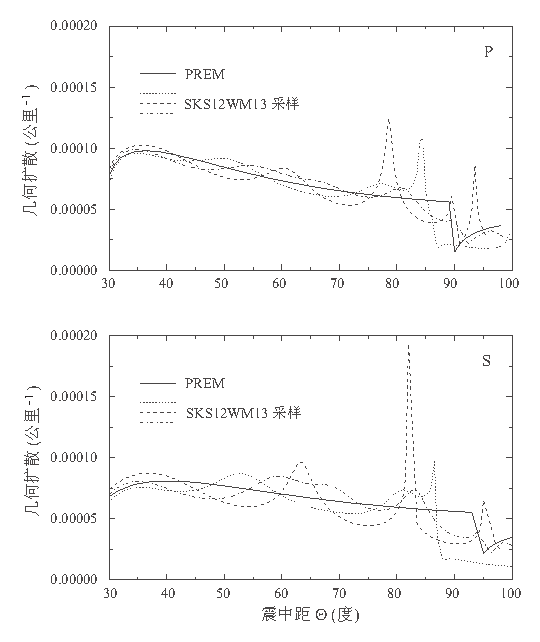
\includegraphics{../figures/chap15/fig08.eps}
\end{center}
\caption[spreading factor]
{\label{15.fig.LTfig3}
Variation of the reciprocal $\sR^{-1}$ of the
geometrical spreading factor~(\ref{15.LTRdef})
with epicentral distance $\Theta$ along a number of
great-circular profiles in model SKS12WM13, compared
with the corresponding variation~(\ref{15.Rsphere}) in PREM.
({\em Top\/}) P waves.  ({\em Bottom\/}) S waves.
The path differences in $\sR^{-1}$ are due to focusing and defocusing of the ray tubes,
caused by the lateral heterogeneity.}
\end{figure}

\subsection{Numerical examples}

\begin{figure}[!t]
\begin{center}
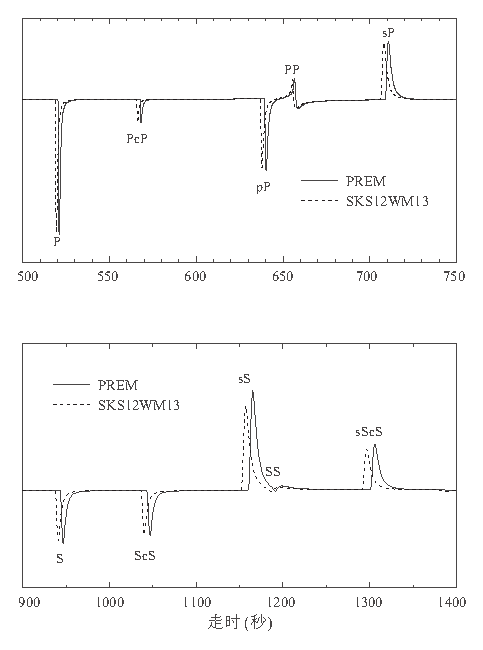
\includegraphics{../figures/chap15/fig09.eps}
\end{center}
\caption[ray theory seismograms]
{\label{15.fig.LTfig4}
Ray-theoretical body-wave seismograms $s(t)$ in models SKS12WM13
and PREM.  The location ${\bf x}_{\rm s}$ and moment tensor
${\bf M}$ are those of the June 9, 1994 deep-focus earthquake
in Bolivia; the receiver ${\bf x}$ is GSN station CCM in Cathedral
Cave, Missouri, at an epicentral distance $\Theta=56.3^{\circ}$.
({\em Top\/}) Radial ($\hat{\mbox{\boldmath $\nu$}}=\hat{\bf r}$)
component.  ({\em Bottom\/}) Transverse ($\hat{\mbox{\boldmath $\nu$}}
=\hat{\bf r}\times\hat{\bf\Theta}$) component.
Travel-time anomalies such as those shown here are the basis
of body-wave tomography.  The twisting of the shear-wave
\index{body-wave tomography}%
\index{tomography!body-wave}%
polarization has been ignored.
}
\end{figure}
Figure~\ref{15.fig.LTfig3} compares a number of great-circular profiles
of $\sR^{-1	}$ versus epicentral distance $\Theta$ in the
three-dimensional Earth model SKS12WM13 (Dziewonski, Liu \& Su
\citeyear{liu&dziewonski96}) with the corresponding variation
in the spherical Earth model PREM (Dziewonski \& Anderson
\citeyear{dziewonski&anderson81}).
The singularities where $\sR^{-1}\rightarrow\infty$ beyond
$\Theta=75^{\circ}$ are due to the presence of small-scale
triplications, produced by the strong lateral heterogeneity
in the lowermost mantle (see Figure~\ref{15.fig.LTfig2}).
Synthetic seismograms $s(t)$ on
models SKS12WM13 and PREM, computed using~(\ref{15.DISP3}),
are compared in Figure~\ref{15.fig.LTfig4}.  The source
is presumed to be impulsive, so that the phases
P, PcP, pP, sP on the radial component and S, ScS, sS,
sScS on the transverse component are all anelastically
broadened Dirac delta pulses of the form $\delta(t-T)*a(t)$.
The surface reflections PP and SS are, on the other hand,
Hilbert-transformed emergent arrivals of the form
$\delta_{\rm H}(t)*a(t)$, due to having passed
through a caustic.  All of the paths between the
\index{Bolivia 1994 earthquake}%
great 1994 Bolivia earthquake and
the receiver
at station CCM in Cathedral Cave, Missouri are
slightly faster in model SKS12WM13 than in PREM;
there are also slight perturbations in the amplitudes of
the pulses, due to variations in the focusing and defocusing of
the associated ray tubes, produced by the lateral heterogeneity.

\section{Ray Perturbation Theory}
\index{ray perturbation theory!body waves|(}%
\label{section:15.9}

Ray theory in an Earth model $\earth+\delta\earth$
that is very nearly spherically symmetric constitutes
a special case, which we investigate in this section.
The deviations from spherical symmetry
must be {\em slight as well as smooth\/} in order for
\index{perturbation!slight}%
\index{perturbation!smooth}%
the results of this {\em ray perturbation theory\/}
to be applicable.

\subsection{Travel time}

As we have seen, Fermat's principle~(\ref{15.Fermat1})
stipulates that the travel time is a stationary functional
of the path between a fixed source $\bx'$ and receiver $\bx$.
This allows us to calculate the travel-time perturbation
$\delta T=T_{\subearth+\delta\subearth}-T_{\subearth}$,
correct to first order, by integration along the
{\em unperturbed ray path\/} in the spherically symmetric
Earth (Julian \& Anderson \citeyear{julian&anderson68}):
\eq \label{15.pertT}
\delta T=-\int_{\subx^{\prime}}^{\subx}v^{-2}\,\delta v\,ds
=-p^{-1}\int_0^{\Theta}r^2v^{-3}\,\delta v\,d\phi.
\en
The final form assumes that the source and receiver
are situated on the equator, as in~(\ref{15.eqrot}).
If there are perturbations $\delta\hspace{-0.1 mm}d$
in the locations of the boundaries in addition to the
volumetric wave-speed perturbations $\delta v$,
then~(\ref{15.pertT}) must be amended:
\eq \label{pertT2}
\delta T\rightarrow \delta T+\sum_d\delta T_d,
\en
where the sum is over all of the boundaries
encountered by the ray.  The nature of the boundary
delay $\delta T_d$ depends upon the type of interaction:
\eq \label{15.pertT3}
\delta T_d=\left\{\begin{array}{ll}
-\delta\hspace{-0.1 mm}d\,
[(v_d^{-2}-p^2d^{-2})^{1/2}]^+_- &
\mbox{transmitted ray} \\
\vspace{-2.0 mm} & \\
-2\hspace{0.3 mm}\delta\hspace{-0.1 mm}d\,
(v_{d+}^{-2}-p^2d^{-2})^{1/2} &
\mbox{topside reflection} \\
\vspace{-2.0 mm} & \\
+2\hspace{0.3 mm}\delta\hspace{-0.1 mm}d\,
(v_{d-}^{-2}-p^2d^{-2})^{1/2} &
\mbox{bottomside reflection.} \\
\end{array}\right.
\en
Equations~(\ref{15.pertT})--(\ref{15.pertT3})
provide a {\em linear\/} relationship between measured travel-time
anomalies $\delta T$ and the lateral heterogeneity $\delta v$ and
$\delta\hspace{-0.1 mm}d$ of the Earth.  These relations are the
basis of linear travel-time tomography.
\index{travel-time tomography}%
\index{tomography!travel-time}%

Figure~\ref{15.fig.LTfig10rhs} compares the linearized
prediction~(\ref{15.pertT}) with the results obtained by exact ray
tracing between a number of source-receiver pairs in Earth
model SKS12WM13.
\begin{figure}[!b]
\begin{center}
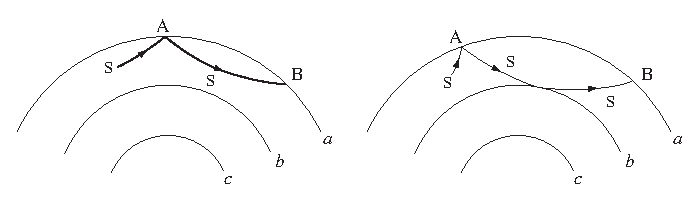
\includegraphics{../figures/chap15/fig10.eps}
\end{center}
\caption[travel time scatter plot]
{\label{15.fig.LTfig10rhs}
Scatter-plot comparison of the travel-time perturbation
$\delta T$ computed using first-order perturbation theory
and exact ray tracing in model SKS12WM13.  Each graph
displays results for 1000 source-receiver paths, between
randomly selected events in the Harvard moment-tensor
catalogue and randomly selected stations in the Global
Seismic Network.  Epicentral distance ranges are as
follows---P: $30^{\circ}\leq\Theta\leq 95^{\circ}$,
S: $30^{\circ}\leq\Theta\leq 80^{\circ}$, PP and SS:
$60^{\circ}\leq\Theta\leq 179^{\circ}$, PcP and ScS:
$10^{\circ}\leq\Theta\leq 75^{\circ}$, PKIKP:
$130^{\circ}\leq\Theta\leq 170^{\circ}$, SKS:
$85^{\circ}\leq\Theta\leq 130^{\circ}$.
}
\end{figure}
First-order perturbation theory consistently overpredicts
the travel-time anomaly $\delta T$ of all refracted and core-reflected
phases such as P, PcP, PKIKP and S, ScS, SKS.  This phenomenon is
an anticipated consequence of Fermat's principle---the geometrical
ray path is the {\em least-time\/} path of any wave that has not
\index{least-time path}%
passed through a caustic.  Minimax phases such as PP and SS do not
\index{minimax phase}%
exhibit such a {\em Fermat bias\/}.  The generally excellent
\index{Fermat bias}%
agreement between the exact and first-order results in
Figure~\ref{15.fig.LTfig10rhs} justifies the continued
use of~(\ref{15.pertT})--(\ref{15.pertT3}) in large-scale global tomographic
investigations.  Non-linear inversion schemes have begun to be developed,
for use in higher-resolution regional-scale investigations
characterized by strong lateral heterogeneity (Sambridge
\citeyear{sambridge90}; Papazachos \& Nolet
\citeyear{papazachos&nolet97a}; \citeyear{papazachos&nolet97b}).

\renewcommand{\thesubsection}{$\!\!\!\raise1.3ex\hbox{$\star$}\!\!$
\arabic{chapter}.\arabic{section}.\arabic{subsection}}
\subsection{Ellipticity correction}
\index{ellipticity correction!body waves|(}%
\renewcommand{\thesubsection}{\arabic{chapter}.\arabic{section}.\arabic{subsection}}

Ellipticity corrections have routinely been applied to
body-wave travel-time measurements for over sixty years
(Bullen \citeyear{bullen37}; \citeyear{bullen63}).
A modern treatment of the problem has been given by
Dziewonski \& Gilbert (\citeyear{dziewonski&gilbert76});
we summarize their findings here.  Let $\psi$ and $\Psi$
be the colatitude and epicentral distance of the running
point along the ray path from $\bx'$ to $\bx$, as illustrated
in Figure~\ref{15.fig.ellip}.
\begin{figure}[!b]
\begin{center}
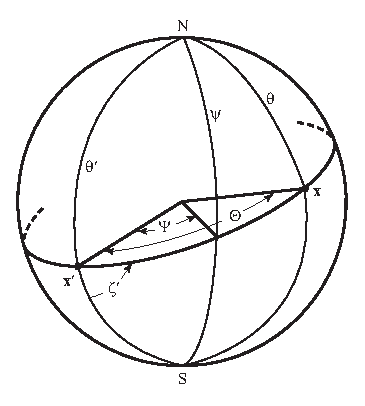
\includegraphics{../figures/chap15/fig11.eps}
\end{center}
\caption[ellipticity correction]
{\label{15.fig.ellip}
Geometrical notation used in the derivation of the ellipticity
correction formula~(\ref{15.ellpert5})--(\ref{15.ellpert6}).
The angles $\theta'$, $\theta$ and $\psi$ are the colatitudes
of the source, the receiver and the integration point along the
ray, respectively. The epicentral coordinates of the integration
point are $\Psi$ and $\zeta'$; the first of these is the angular
distance from the source, and the second is the takeoff azimuth
of the path to the receiver, measured counterclockwise from due
south as usual.
}
\end{figure}
These two angular arclengths are related to the
source colatitude $\theta'$ and the receiver azimuth $\zeta'$ by
\eq \label{15.ellpert2}
\cos\psi=\cos\theta'\cos\Psi-\sin\theta'\sin
\Psi\cos\zeta'.
\en
The Earth's hydrostatic ellipticity is a degree-two zonal
perturbation of the form~(\ref{14.ellperts}):
\eq \label{15.ellpert3}
\delta v=\twothirds r\eps\dot{v}P_2(\cos\psi),\qquad
\delta\hspace{-0.1 mm}d=-\twothirds d\eps_dP_2(\cos\psi).
\en
The Legendre polynomial $P_2(\cos\psi)$ can be expressed in terms
of the running epicentral distance $\Psi$ and the fixed colatitude
$\theta'$ and azimuth $\zeta'$ using the spherical-harmonic
addition theorem~(\ref{B.realaddth}):
\eqa \label{15.ellpert4} \lefteqn{
P_2(\cos\psi)=\sum_{m=0}^2(-1)^m(2-\delta_{m0})
\left[\frac{(2-m)!}{(2+m)!}\right]} \nonumber \\
&&\mbox{}\qquad\qquad\qquad\times P_{2m}
(\cos\Psi)P_{2m}(\cos\theta')\cos m\zeta'.
\ena
Upon substituting~(\ref{15.ellpert3})--(\ref{15.ellpert4})
into~(\ref{15.pertT})--(\ref{15.pertT3}) we can write the
ellipticity travel-time perturbation as a sum of three associated
Legendre functions:
\eq \label{15.ellpert5}
\delta T^{\rm ell}=\sum_{m=0}^2\delta T_m(\Theta,h)\,
P_{2m}(\cos\theta')\cos m\zeta'.
\en
The three coefficients $\delta T_0$, $\delta T_1$,
$\delta T_2$ are ray-specific functions of the
epicentral distance $\Theta$ and
source depth $h$, given by
\eqa \label{15.ellpert6} \lefteqn{
\delta T_m=-\twothirds (-1)^m(2-\delta_{m0})
\left[\frac{(2-m)!}{(2+m)!}\right]} \nonumber \\
&&\mbox{}\times\left\{p^{-1}\int_0^{\Theta}r^3v^{-3}\eps\dot{v}
P_2(\cos\Psi)\,d\Psi\right. \nonumber \\
&&\mbox{}-\sum_d^{\rm tran}d\eps_d\,
[(v_d^{-2}-p^2d^{-2})^{1/2}]^+_-
\,P_2(\cos\Psi_d) \nonumber \\
&&\mbox{}\mp\left.\sum_d^{\rm refl}2d\eps_d
(v_{d\pm}^{-2}-p^2d^{-2})^{1/2}
P_2(\cos\Psi_d)\right\}.
\ena
The first sum is over all of the boundaries
through which the ray is transmitted, whereas the second is over all
of the boundaries from which it is reflected; the top and bottom
signs correspond to topside and bottomside reflections, respectively.
Computer code to evaluate the coefficients~(\ref{15.ellpert6}) is
documented in Doornbos (\citeyear{doornbos88}).  The {\em IASPEI 1991
Seismological Tables\/} (Kennett \citeyear{kennett91}) include
listings of $\delta T_0$, $\delta T_1$, $\delta T_2$ for selected
phases, computed using this code.
Kennett \& Gudmundsson (\citeyear{kennett&gudmundsson96}) discuss the modifications
needed to extend the results~(15.271)--(15.272) to non-geometrical
phases such as ${\rm P}_{\rm diff}$ in the core shadow;
these authors also show how to compute the ellipticity
corrections for compound phases such as PP by combining
results for the various legs. It should be noted that all of these
references follow the original convention of Dziewonski \& Gilbert
(\citeyear{dziewonski&gilbert76}) rather than the one employed here;
in particular, the azimuth is measured clockwise from north rather
than counterclockwise from south, and the normalization of the
Legendre functions in the equivalent of~(\ref{15.ellpert5}) is unusual.
\index{ellipticity correction!body waves|)}%

\renewcommand{\thesubsection}{$\!\!\!\raise1.3ex\hbox{$\star$}\!\!$
\arabic{chapter}.\arabic{section}.\arabic{subsection}}
\subsection{Ray geometry}
\index{ray geometry!body-wave|(}%
\renewcommand{\thesubsection}{\arabic{chapter}.\arabic{section}.\arabic{subsection}}

Small changes in the geometry of a spherical-Earth ray
can be determined by means of a perturbation analysis
of Hamilton's equations~(\ref{15.Hameqn}).  Alternatively,
it is possible to perturb the equivalent system of four
equations in ray-centered coordinates; the results of
such a ray-centered perturbation
analysis are presented by Farra \& Madariaga
(\citeyear{farra&madariaga87}) and Coates \& Chapman
(\citeyear{coates&chapman90}).  This section
describes a third variant of ray perturbation theory,
due to Liu \& Tromp (\citeyear{liu&tromp96}).  In this
method, which is particularly well suited for global
seismological applications, perturbation theory
is applied to the four spherical polar ray-tracing
equations~(\ref{15.LTeq1})--(\ref{15.LTeq4}).
We shall restrict attention initially to the case
of an Earth model with spherically symmetrical
discontinuities; the effect of a slight
boundary perturbation $\delta\hspace{-0.1 mm}d$
will be considered briefly in Section~15.9.4.

Supposing the unperturbed spherical-Earth ray to lie in the equatorial plane,
with the local radius $r$ and incidence angle $i$ determined
by~(\ref{15.LTri}), we consider perturbations of the form
\eqa \label{15.LTperts} \lefteqn{
r\rightarrow r+\delta r,
\qquad
\theta\rightarrow\pi/2+\delta\hspace{-0.1 mm}\theta,
\qquad
i\rightarrow i+\delta i,
\qquad
\zeta\rightarrow\pi/2+\delta\zeta.} \nonumber \\
&&\mbox{}
\ena
Upon substituting~(\ref{15.LTperts})
into~(\ref{15.LTeq1})--(\ref{15.LTeq4})
and ignoring second-order terms,
we obtain a system of linear equations
governing the evolution of $\delta r$,
$\delta\hspace{-0.1 mm}\theta$,
$\delta i$ and $\delta\zeta$ along a perturbed ray:
\eq \label{15.LT7r}
\frac{d}{d\phi}\delta r=\cot\hspace{-0.2 mm}
i\hspace{0.9 mm}\delta r-r(\sin i)^{-2}\,\delta i,
\en
\eq \label{15.LT7theta}
\frac{d}{d\phi}\delta\hspace{-0.1 mm}\theta=-\delta\zeta,
\en
\vspace{-2.0 mm}
\eqa \label{15.LT7i}
\lefteqn{
\frac{d}{d\phi}\delta i=(rv^{-1}\ddot{v}-
rv^{-2}\dot{v}^2+v^{-1}\dot{v})\,\delta r
+rv^{-1}\p_r\delta v} \nonumber \\
&&\mbox{}-v^{-1}\cot i\hspace{0.9 mm}
\p_\phi\delta v-rv^{-2}\dot{v}\,\delta v,
\ena
\eq \label{15.LT7zeta}
\frac{d}{d\phi}\delta\zeta=\delta\hspace{-0.1 mm}\theta
+(\sin i)^{-2}v^{-1}\p_\theta\delta v.
\en
The associated perturbed boundary conditions require that
\begin{displaymath}
[\tan i\hspace{0.9 mm}\delta r]^+_-=0,\qquad
[\delta\hspace{-0.1 mm}\theta]^+_-=0,\qquad[\delta\zeta]^+_-=0,
\end{displaymath}
\eq \label{15.LT7boun}
[\cot i\hspace{0.9 mm}\delta i-(v^{-1}\dot{v}-r^{-1})
\,\delta r-v^{-1}\delta v]^+_-=0
\en
at every spherical discontinuity.  The term $-v^{-1}\delta v$
in the final condition~(\ref{15.LT7boun}) arises because
the wave-speed perturbations experienced by the incident
wave and the reflected or transmitted wave may differ.
It is noteworthy that the equations and boundary conditions
governing $\delta r$ and $\delta i$ are decoupled from those
governing $\delta\hspace{-0.1 mm}\theta$ and $\delta\zeta$.

Let us solve for the out-of-plane perturbations
$\delta\hspace{-0.1 mm}\theta$ and $\delta\zeta$ first.
We begin by rewriting equations~(\ref{15.LT7theta})
and~(\ref{15.LT7zeta}) in a convenient $2\times 2$
matrix notation:
\eq \label{15.LT7vector}
\frac{d\ssy}{d\phi}=\ssA\ssy+\ssf,
\en
where
\eq
\ssy=\left(\begin{array}{c}
\delta\theta \\
\vspace{-2.0 mm} \\
\delta\zeta
\end{array}\right),
\qquad
\ssf=\left(\begin{array}{c}
0 \\
\vspace{-2.0 mm} \\
(\sin i)^{-2}v^{-1}\p_\theta\delta v
\end{array}\right),
\en
\eq
\ssA=\left(\begin{array}{lr}
0 & -1 \\
\vspace{-2.0 mm} & \\
1 & 0
\end{array}\right).
\en
It is easily verified by direct substitution that the
solution to the inhomogeneous equation~(\ref{15.LT7vector}) is
\eqa \label{15.LT7solution2} \lefteqn{
\ssy(\phi)=\ssP(\phi,0)\left[\int_0^{\phi}\ssP^{-1}(\tilde{\phi},0)
\hspace{0.4 mm}\ssf(\tilde{\phi})\,d\tilde{\phi}+\ssy(0)\right]}
\nonumber \\
&&\mbox{}\hspace{-0.5 mm}=\int_0^{\phi}\ssP(\phi,\tilde{\phi})
\hspace{0.4 mm}\ssf(\tilde{\phi})\,d\tilde{\phi}
+\ssP(\phi,0)\hspace{0.4 mm}\ssy(0).
\ena
Here $\ssP$ is the $2\times 2$ propagator matrix satisfying
\eq \label{15.LTpropdef}
\frac{d\hspace{0.2 mm}\ssP}{d\phi}=\ssA\ssP,\qquad\ssP(\phi,\phi)=\ssI.
\en
The second equality in~(\ref{15.LT7solution2}) follows from
the inverse-propagator identity
\eq
\ssP(\phi,0)\hspace{0.4 mm}\ssP^{-1}
(\tilde{\phi},0)=\ssP(\phi,0)\hspace{0.4 mm}\ssP
(0,\tilde{\phi})=\ssP(\phi,\tilde{\phi}).
\en
The propagator from one arbitrary point
$0\leq\tilde{\phi}\leq\Theta$ to another
$0\leq\phi\leq\Theta$ is given explicitly by
\eq\label{15.LTpropsincos}
\ssP(\phi,\tilde{\phi})=\left(\begin{array}{lr}
\cos(\phi-\tilde{\phi}) & -\sin(\phi-\tilde{\phi}) \\
\vspace{-2.0 mm} & \\
\sin(\phi-\tilde{\phi}) & \cos(\phi-\tilde{\phi})
\end{array}\right).
\en
The perturbed ray is required to emanate from the same source
and hit the same receiver as the unperturbed ray; that is,
\eq \label{15.LT7bc}
\ssy(0)=
\left(\begin{array}{c}
0 \\
\delta\zeta'
\end{array}\right),
\qquad
\ssy(\Theta)=
\left(\begin{array}{c}
0 \\
\delta\zeta
\end{array}\right),\label{eq:7.bc}
\en
where $\delta\zeta'$ and $\delta\zeta$ denote the
perturbed out-of-plane takeoff and arrival angles, respectively.
Upon inserting~(\ref{15.LT7bc}) into~(\ref{15.LT7solution2}),
we obtain the closed-form representations
\eq \label{15.LT7takeoff1}
\delta\zeta'=-(\sin\Theta)^{-1}\int_0^\Theta\sin(\Theta-\phi)
(\sin i)^{-2}v^{-1}\p_\theta\hspace{-0.1 mm}\delta v\,d\phi,
\en
\eq \label{15.LT7arrival1}
\delta\zeta=(\sin\Theta)^{-1}\int_0^\Theta\sin\phi
\,(\sin i)^{-2}v^{-1}\p_\theta\delta v\,d\phi.
\en
Equations~(\ref{15.LT7takeoff1}) and~(\ref{15.LT7arrival1})
determine the initial and final perturbations $\delta\zeta'$
and $\delta\zeta$ in terms of the wave-speed gradient
$\p_{\theta}\delta v$ perpendicular to the spherical-Earth
ray plane.  The integration is performed along the
unperturbed ray $r(\phi)$, $i(\phi)$.  The complete
solution~(\ref{15.LT7solution2}) at intermediate points
$0\leq\phi\leq\Theta$ is
\eq \label{15.LT7p1}
\delta\hspace{-0.1 mm}\theta(\phi)=-\int_0^\phi\sin(\phi-\tilde{\phi})
(\sin\tilde{\imath})^{-2}\tilde{v}^{-1}
\p_\theta\delta\tilde{v}\,d\tilde{\phi}-\delta\zeta'\sin\phi,
\en
\eq \label{15.LT7p2}
\delta\zeta(\phi)=\int_0^\phi\cos(\phi-\tilde{\phi})
(\sin\tilde{\imath})^{-2}\tilde{v}^{-1}
\p_\theta\delta\tilde{v}\,d\tilde{\phi}+\delta\zeta'\cos\phi,
\en
where the tildes denote evaluation at the dummy variable $\tilde{\phi}$.
Note that $\delta\hspace{-0.1 mm}\theta(0)=\delta\theta(\Theta)=0$
whereas $\delta\zeta(0)=\delta\zeta'$ and $\delta\zeta(\Theta)=
\delta\zeta$, as expected.

Next, we determine the in-plane perturbations $\delta r$ and $\delta i$.
The governing equations~(\ref{15.LT7r}) and~(\ref{15.LT7i}) may be
written in a matrix form analogous to~(\ref{15.LT7vector}):
\eq \label{15.LTdiffeq}
\frac{d\ssy}{d\phi}=\ssA\ssy+\ssf.
\en
To account for the jumps $[\delta r]^+_-$ and $[\delta i]^+_-$
at interfaces, we are required to solve equation~(\ref{15.LTdiffeq})
subject to an inhomogeneous continuity condition at every
boundary interaction point along the unperturbed ray:
\eq \label{15.LTbo}
[\ssB\ssy+\ssb]^+_-=\sszero.
\en
The $2\times 1$ column vectors $\ssy$, $\ssb$, $\ssf$ and the
$2\times 2$ matrices $\ssA$, $\ssB$ in
equations~(\ref{15.LTdiffeq})--(\ref{15.LTbo})
are defined by
\eq
\ssy=\left(\begin{array}{c}
\delta r \\
\vspace{-2.0 mm} \\
\delta i
\end{array}\right),\qquad
\ssb=\left(\begin{array}{c}
0 \\
\vspace{-2.0 mm} \\
-v^{-1}\delta v
\end{array}\right),
\en
\eq \label{15.LTssf}
\ssf=\left(\begin{array}{c}
0 \\
\vspace{-2.0 mm} \\
rv^{-1}\p_r\delta v-\cot i\,v^{-1}\p_\phi\delta v
-rv^{-2}\dot{v}\,\delta v
\end{array}\right),
\en
\eq \label{15.LTssA2}
\ssA=\left(\begin{array}{cc}
\cot i & -r(\sin i)^{-2} \\
\vspace{-2.0 mm} & \\
rv^{-1}\ddot{v}-
rv^{-2}\dot{v}^2+v^{-1}\dot{v} & 0
\end{array}\right),
\en
\eq \label{15.LTssB}
\ssB=\left(\begin{array}{cc}
\tan i & 0 \\
\vspace{-2.0 mm} & \\
-v^{-1}\dot{v}+r^{-1} & \cot i
\end{array}\right).
\en
In this case the $2\times 2$ propagator matrix $\ssP$
must satisfy an additional boundary constraint; the complete
set of defining relations is
\eq \label{15.LTpropdef2}
\frac{d\hspace{0.2 mm}\ssP}{d\phi}=\ssA\ssP,\qquad
[\ssB\ssP]^+_-=\sszero,\qquad
\ssP(\phi,\phi)=\ssI.
\en
The elements of the in-plane propagator are the four partial derivatives
\eq \label{15.LT7P2}
\ssP(\phi,\tilde{\phi})=\left(\begin{array}{cc}
\p_{\tilde{r}}r(\phi,\tilde{\phi}) & \p_{\tilde{\imath}}r(\phi,\tilde{\phi}) \\
\vspace{-1.0 mm} & \\
\p_{\tilde{r}}i(\phi,\tilde{\phi}) & \p_{\tilde{\imath}}i(\phi,\tilde{\phi})
\end{array}\right),
\en
where $\tilde{r}=r(\tilde{\phi})$ and $\tilde{\imath}=i(\tilde{\phi})$.
The solution to equations~({\ref{15.LTdiffeq})--(\ref{15.LTbo})
can be written in terms of the matrix~(\ref{15.LT7P2}) and its
inverse,
\eq \label{15.LT7P3}
\ssP^{-1}(\phi,\tilde{\phi})=
\frac{1}{{\rm det}\,\ssP(\phi,\tilde{\phi})}
\left(\begin{array}{cc}
\p_{\tilde{\imath}}i(\phi,\tilde{\phi}) &
-\p_{\tilde{\imath}}r(\phi,\tilde{\phi}) \\
\vspace{-1.0 mm} & \\
-\p_{\tilde{r}}i(\phi,\tilde{\phi}) &
\p_{\tilde{r}}r(\phi,\tilde{\phi})
\end{array}\right),
\en
in the form
\eqa \label{15.LT7solution3}
\lefteqn{
\ssy(\phi)=\ssP(\phi,0)\left[\int_0^{\phi}
\ssP^{-1}(\tilde{\phi},0)\hspace{0.4 mm}\ssf(\tilde{\phi})\,d\tilde{\phi}
+\ssy(0)\right.} \nonumber \\
&&\qquad\qquad\mbox{}
\left.+\sum_d\ssP^{-1}(\phi_d,0)\left(\ssB_d^{\rm out}\right)^{-1}
(\ssb_d^{\rm inc}-\ssb_d^{\rm out})\right] \nonumber \\
&&\mbox{}\hspace{-0.5 mm}
=\int_0^{\phi}\ssP(\phi,\tilde{\phi})\hspace{0.4 mm}
\ssf(\tilde{\phi})\,\tilde{d\phi}
+\ssP(\phi,0)\hspace{0.4 mm}\ssy(0) \nonumber \\
&&\mbox{}\qquad\qquad
+\sum_d\ssP(\phi,\phi_d)\left(\ssB_d^{\rm out}\right)^{-1}
(\ssb_d^{\rm inc}-\ssb_d^{\rm out}).
\ena
The summation is over all of the boundaries encountered by
the unperturbed ray; the superscripts
inc and out denote evaluation upon the incident and outgoing
sides of the discontinuity.  Only when $\delta v^{\rm inc}$
and $\delta v^{\rm out}$ are different do the boundary terms
contribute; in that case, their effect can be quite significant.

Once again we demand that the perturbed and unperturbed rays
start from the same source and hit the same receiver:
\eq \label{15.LT7bc2}
\ssy(0)=
\left(\begin{array}{c}
0 \\
\vspace{-2.0 mm} \\
\delta i'
\end{array}\right),
\qquad
\ssy(\Theta)=
\left(\begin{array}{c}
0 \\
\vspace{-2.0 mm} \\
\delta i
\end{array}\right).
\en
Upon inserting the boundary conditions~(\ref{15.LT7bc2})
into~(\ref{15.LT7solution3}) and noting that $\tilde{r}(0)=r'$
and $\tilde{\imath}(0)=i'$, we find that the perturbed takeoff
angle $\delta i'$ and arrival angle $\delta i$ are given by
\eqa \label{15.LT7takeoff2}
\lefteqn{
\delta i'=\frac{1}{\p_{i'}r(\Theta)}
\int_0^{\Theta}D^{-1}(\phi)\,[\p_{r'}r(\Theta)
\p_{i'}r(\phi)-\p_{i'}r(\Theta)
\p_{r'}r(\phi)]} \nonumber \\
&&\mbox{}\qquad
\times[rv^{-1}\p_r\delta v-\cot i\,v^{-1}\p_\phi\delta v
-rv^{-2}\dot{v}\,\delta v]\,d\phi \nonumber \\
&&\mbox{}
+\frac{1}{\p_{i'}r(\Theta)}
\sum_dD^{-1}(\phi_d^{\rm out}) \nonumber \\
&&\mbox{}\qquad
\times[\p_{r'}r(\Theta)
\p_{i'}r(\phi_d^{\rm out})-\p_{i'}r(\Theta)
\p_{r'}r(\phi_d^{\rm out})] \nonumber \\
&&\mbox{}\qquad
\times\tan i^{\rm out}_d[(v^{-1}\delta v)_d^{\rm out}
-(v^{-1}\delta v)_d^{\rm inc}],
\ena
\eqa \label{15.LT7arrival2}
\lefteqn{
\delta i=\frac{D(\Theta)}{\p_{i'}r(\Theta)}
\int_0^{\Theta}D^{-1}(\phi)\,\p_{i'}r(\phi)} \nonumber \\
&&\mbox{}\qquad
\times[rv^{-1}\p_r\delta v-\cot i\,v^{-1}\p_\phi\delta v
-rv^{-2}\dot{v}\,\delta v]\,d\phi \nonumber \\
&&\mbox{}
+\frac{D(\Theta)}{\p_{i'}r(\Theta)}
\sum_dD^{-1}(\phi_d^{\rm out})\,\p_{i'}r(\phi_d^{\rm out}) \nonumber \\
&&\mbox{}\qquad
\tan i^{\rm out}_d[(v^{-1}\delta v)_d^{\rm out}
-(v^{-1}\delta v)_d^{\rm inc}],
\ena
where
\eq
D(\phi)=\p_{r'}r(\phi)
\p_{i'}i(\phi)-\p_{i'}r(\phi)
\p_{r'}i(\phi).
\en
Equations~(\ref{15.LT7takeoff2})--(\ref{15.LT7arrival2})
determine the perturbations $\delta i'$, $\delta i$
in terms of the in-plane wave-speed gradients $\p_r\delta v$,
$\p_{\phi}\delta v$ and the boundary contrasts
$(v^{-1}\delta v)_d^{\rm out}
-(v^{-1}\delta v)_d^{\rm inc}$.
In shooting to find the geometrical rays
\index{shooting!initial guess}%
between a given source and receiver,
it is advantageous to use~(\ref{15.LT7takeoff1})
and~(\ref{15.LT7takeoff2}) as first estimates
of the initial takeoff azimuth $\zeta_0^{\prime}
=\pi/2+\delta\zeta'$ and incidence angle $i_0^{\prime}
=i'+\delta i'$; this can substantially decrease the
number of iterations of~(\ref{15.LTNewton}) needed
to hit the receiver.
\begin{sidewaysfigure}
\begin{center}
\rotatebox{270}
{
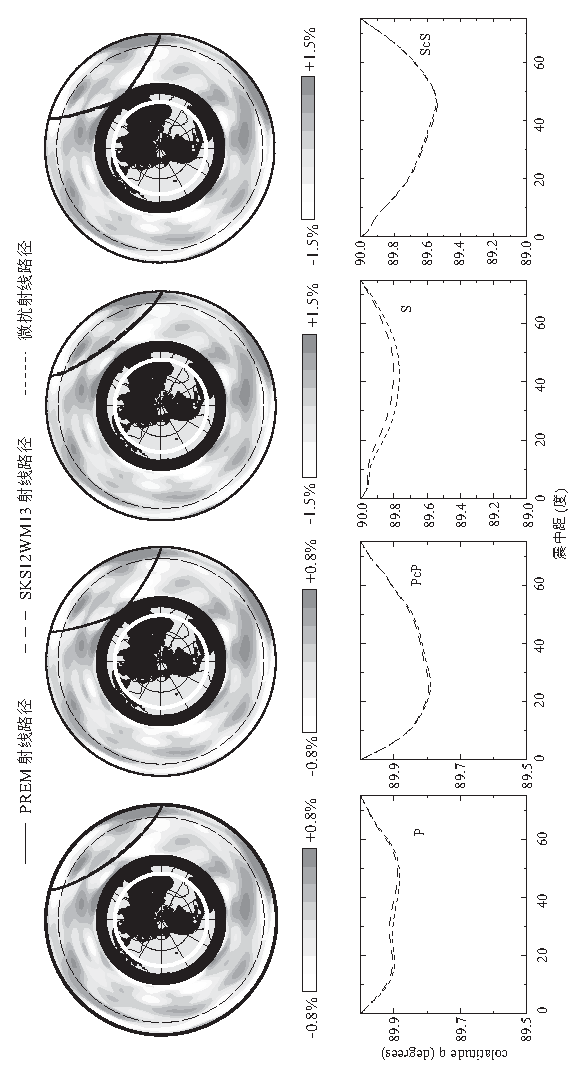
\includegraphics{../figures/chap15/fig12.eps}
}
\end{center}
\caption[liu&tromp Fig 9]{
Comparison of the exact ({\em long dashed line\/}) and
perturbation-theoretical ({\em short dashed line\/}) ray paths
in model SKS12WM13. The unperturbed ray path
in PREM is also shown ({\em solid line\/}).  The source
is situated on the equator and Greenwich Meridian, and the
receiver is situated due east at an epicentral distance
$\Theta=75^{\circ}$.  ({\em Top\/}) P, PcP, S and ScS
rays projected onto a cross-section of the source-receiver
great-circle plane. Shading depicts the relative wave-speed
perturbations $-0.8\%\leq\delta\hspace{-0.1 mm}\alpha/\alpha\leq 0.8\%$
and $-1.5\%\leq\delta\hspace{-0.2 mm}\beta/\beta\leq 1.5\%$.
({\em Bottom\/}) Projection of the same ray paths onto the
surface of the Earth.
}
\label{15.fig.LTfig9}
\end{sidewaysfigure}

The complete geometry of the perturbed ray is determined by
equations~(\ref{15.LT7p1})--(\ref{15.LT7p2}) together with
\eqa \label{15.LT7p3}
\lefteqn{
\delta r(\phi)=
\int_0^{\phi}D^{-1}(\tilde{\phi})\,
[-\p_{r'}r(\phi)\p_{i'}r(\tilde{\phi})
+\p_{i'}r(\phi)\p_{r'}r(\tilde{\phi})]} \nonumber \\
&&\mbox{}\qquad
\times[rv^{-1}\p_r\delta v-\cot i\,v^{-1}\p_\phi\delta v
-rv^{-2}\dot{v}\,\delta v]\,d\phi \nonumber \\
&&\mbox{}
+\sum_dD^{-1}(\phi_d^{\rm out}) \nonumber \\
&&\mbox{}\qquad\times
[-\p_{r'}r(\phi)
\p_{i'}r(\phi_d^{\rm out})+\p_{i'}r(\phi)
\p_{r'}r(\phi_d^{\rm out})] \nonumber \\
&&\mbox{}\qquad
\times\tan i^{\rm out}_d[(v^{-1}\delta v)_d^{\rm out}
-(v^{-1}\delta v)_d^{\rm inc}]
+\delta i'\,\p_{i'}r(\phi),
\ena
\eqa \label{15.LT7p4}
\lefteqn{
\delta i(\phi)=
\int_0^{\phi}D^{-1}(\tilde{\phi})\,
[-\p_{r'}i(\phi)\p_{i'}r(\tilde{\phi})
+\p_{i'}i(\phi)\p_{r'}r(\tilde{\phi})]} \nonumber \\
&&\mbox{}\qquad
\times[rv^{-1}\p_r\delta v-\cot i\,v^{-1}\p_\phi\delta v
-rv^{-2}\dot{v}\,\delta v]\,d\phi \nonumber \\
&&\mbox{}
+\sum_dD^{-1}(\phi_d^{\rm out}) \nonumber \\
&&\mbox{}\qquad\times
[-\p_{r'}i(\phi)
\p_{i'}r(\phi_d^{\rm out})+\p_{i'}i(\phi)
\p_{r'}r(\phi_d^{\rm out})] \nonumber \\
&&\mbox{}\qquad
\times\tan i^{\rm out}_d[(v^{-1}\delta v)_d^{\rm out}
-(v^{-1}\delta v)_d^{\rm inc}]
+\delta i'\,\p_{i'}i(\phi),
\ena
where the summations are now carried out only over the
discontinuities lying between the
source and the instantaneous point $\phi$.
It is easily verified that
$\delta r(0)=\delta r(\Theta)=0$
and $\delta i(0)=\delta i'$,
$\delta i(\Theta)=\delta i$.
Figure~\ref{15.fig.LTfig9} compares the results
of exact and first-order ray tracing between a
fixed source and receiver in model SKS12WM13.
In general, perturbation theory predicts the geometry
of rays in such a smooth ($s_{\rm max}=12$) Earth model very well.

Figures~\ref{15.fig.takeoff1} and~\ref{15.fig.takeoff2}
compare the exact and first-order incidence angle and
azimuth anomalies $\delta i'$ and $\delta\zeta'$ at the
source, for a number of ray paths in model SKS12WM13.
Figures~\ref{15.fig.arrival1} and~\ref{15.fig.arrival2}
show a similar comparison of the two arrival-angle
anomalies $\delta i$ and $\delta\zeta$ at the receiver.
The large magnitude of the term $(\sin i)^{-2}$ makes
the out-of-plane perturbations~(\ref{15.LT7takeoff1})
and~(\ref{15.LT7arrival1}) of steeply propagating
waves particularly sensitive to transverse gradients
$\p_{\theta}\delta v$.  For this reason, the reflected
phases PcP and ScS exhibit takeoff and arrival anomalies
$\delta\zeta'$, $\delta\zeta$ that are approximately twice
as large as those of the turning phases P and S.
\begin{figure}
\begin{center}
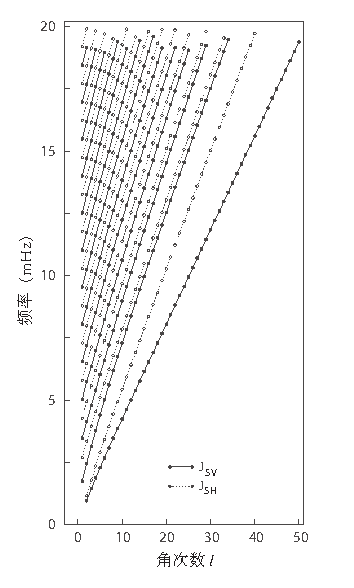
\includegraphics{../figures/chap15/fig13.eps}
\end{center}
\caption[takeoff angle 1]
{\label{15.fig.takeoff1}
Scatter-plot comparison of the incidence-angle anomaly
$\delta i'$ at the source, computed using first-order
perturbation theory and exact ray tracing in model SKS12WM13.
Each graph displays results for 1000 randomly selected
source-receiver paths; the associated travel-time perturbations
$\delta T$ are compared in Figure~\ref{15.fig.LTfig10rhs}.
See Figure~15.15 for the corresponding anomaly $\delta i$ at the receiver.
}
\end{figure}
\begin{figure}
\begin{center}
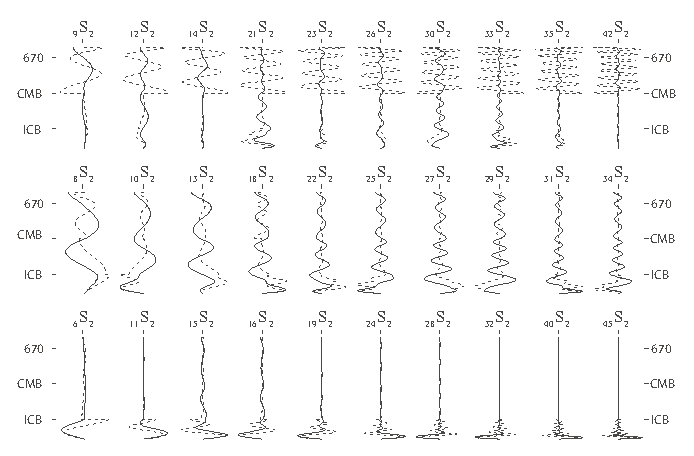
\includegraphics{../figures/chap15/fig14.eps}
\end{center}
\caption[takeoff angle 2]
{\label{15.fig.takeoff2}
Scatter-plot comparison of the the azimuthal takeoff-angle
anomaly $\delta\zeta'$, computed using first-order
perturbation theory and exact ray tracing in model SKS12WM13.
See Figure~15.16 for the corresponding anomaly $\delta\zeta$ at the receiver.
}
\end{figure}
\begin{figure}
\begin{center}
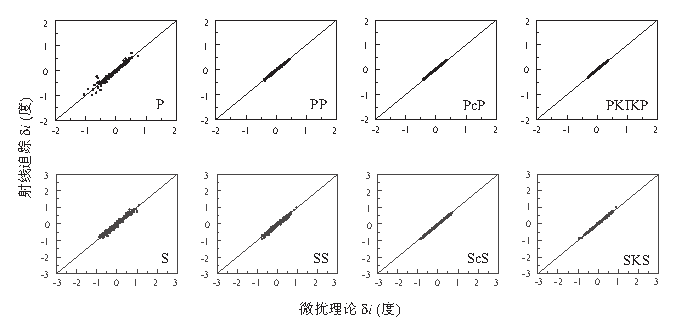
\includegraphics{../figures/chap15/fig15.eps}
\end{center}
\caption[arrival angle 1]
{\label{15.fig.arrival1}
Same as Figure~\ref{15.fig.takeoff1} for the observable incidence-angle
anomaly $\delta i$ at the receiver.
Each scatter plot displays results for 1000 randomly selected source-receiver paths.}
\end{figure}
\begin{figure}
\begin{center}
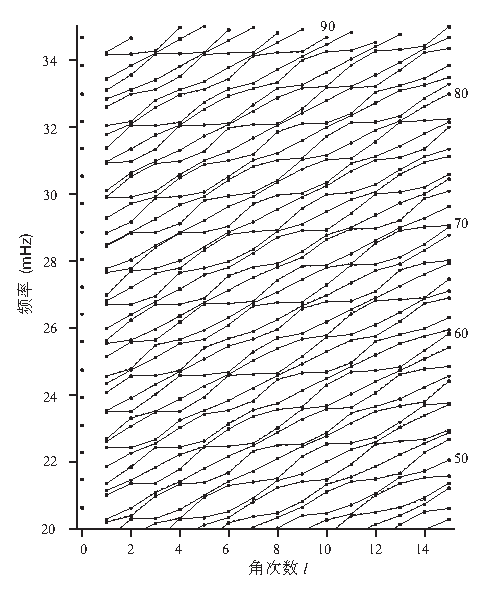
\includegraphics{../figures/chap15/fig16.eps}
\end{center}
\caption[arrival 2]
{\label{15.fig.arrival2}
Same as Figure~\ref{15.fig.takeoff2} for the azimuthal
arrival-angle anomaly $\delta\zeta$.
The epicentral distance ranges in all four Figures~15.13--15.16
are the same as
in Figure~\ref{15.fig.LTfig10rhs}---P: $30^{\circ}\leq\Theta\leq 95^{\circ}$,
S: $30^{\circ}\leq\Theta\leq 80^{\circ}$, PP and SS:
$60^{\circ}\leq\Theta\leq 179^{\circ}$, PcP and ScS:
$10^{\circ}\leq\Theta\leq 75^{\circ}$, PKIKP:
$130^{\circ}\leq\Theta\leq 170^{\circ}$, SKS:
$85^{\circ}\leq\Theta\leq 130^{\circ}$.}
\end{figure}
\index{ray geometry!body-wave|)}%

\renewcommand{\thesubsection}{$\!\!\!\raise1.3ex\hbox{$\star$}\!\!$
\arabic{chapter}.\arabic{section}.\arabic{subsection}}
\subsection{Boundary topography}
\renewcommand{\thesubsection}{\arabic{chapter}.\arabic{section}.\arabic{subsection}}

The effects of a slight perturbation $\delta\hspace{-0.1 mm}d$
in the locations of the initially spherical discontinuities
have been treated by Liu \& Tromp (\citeyear{liu&tromp96}).
We simply quote their results here.  The takeoff-angle and
arrival-angle perturbations~(\ref{15.LT7takeoff1})--(\ref{15.LT7arrival1})
and~(\ref{15.LT7takeoff2})--(\ref{15.LT7arrival2}) exhibit additional
boundary contributions.  The out-of-plane and in-plane deflections
depend upon the transverse $\p_\theta$ and longitudinal $\p_\phi$
gradients in topography, respectively:
\eqa \label{15.LTtopog1} \lefteqn{
\delta\zeta'\rightarrow\delta\zeta'-(\sin\Theta)^{-1}\sum_d
\sin(\Theta-\phi_d)} \nonumber \\
&&\mbox{}\qquad
\times(\cot i_d^{\rm out}-\cot i_d^{\rm inc})
\,\p_{\theta}\hspace{-0.4 mm}\ln\delta\hspace{-0.1 mm}d,
\ena
\eqa \label{15.LTtopog2} \lefteqn{
\delta\zeta\rightarrow\delta\zeta+(\sin\Theta)^{-1}\sum_d
\sin\phi_d(\cot i_d^{\rm out}-\cot i_d^{\rm inc})
\,\p_{\theta}\hspace{-0.4 mm}\ln\delta\hspace{-0.1 mm}d,}
\ena
\eqa \label{15.LTtopog3} \lefteqn{
\delta i'\rightarrow\delta i'-\frac{1}{\p_{i'}r(\Theta)}
\sum_dD^{-1}(\phi_d^{\rm out})} \nonumber \\
&&\mbox{}\qquad
\times[\p_{r'}r(\Theta)
\p_{i'}r(\phi_d^{\rm out})-\p_{i'}r(\Theta)
\p_{r'}r(\phi_d^{\rm out})] \nonumber \\
&&\mbox{}\qquad
\times\tan i^{\rm out}_d(\cot i_d^{\rm out}-\cot i_d^{\rm inc})\,
\p_{\phi}\hspace{-0.4 mm}\ln\delta\hspace{-0.1 mm}d,
\ena
\eqa \label{15.LTtopog4} \lefteqn{
\delta i\rightarrow\delta i-\frac{D(\Theta)}{\p_{i'}r(\Theta)}
\sum_dD^{-1}(\phi_d^{\rm out})\,\p_{i'}r(\phi_d^{\rm out})} \nonumber \\
&&\mbox{}\qquad
\times\tan i^{\rm out}_d(\cot i_d^{\rm out}-\cot i_d^{\rm inc})\,
\p_{\phi}\hspace{-0.4 mm}\ln\delta\hspace{-0.1 mm}d.
\ena
The arrival-angle anomalies $\delta i$ and $\delta\zeta$
at the receiver can be measured by means of a
polarization analysis, applied to a single
three-component recording or to a suite of
recordings from a tightly spaced array.
The above results
enable such data to be used as supplemental constraints in
global travel-time inversion studies; the dependence of
$\delta\zeta$ and $\delta i$ upon the volumetric and
topographic gradients $\p_r\delta v$, $\p_\theta\delta v$,
$\p_\phi\delta v$ and $\p_\theta\delta\hspace{-0.1 mm}d$,
$\p_\phi\delta\hspace{0.1 mm}d$ is strictly linear.
The effect of a possible source mislocation
$\delta r'$, $\delta\hspace{-0.1 mm}\theta'$
can be accounted for by adding terms $(\sin\Theta)^{-1}
\delta\hspace{-0.1 mm}\theta'$ and
$-[D(\Theta)/\p_{i'}r(\Theta)]\,\delta r'$ to the right sides of
equations~(\ref{15.LTtopog2}) and~(\ref{15.LTtopog4}), respectively.

The ray-geometry equations~(\ref{15.LT7p1})--(\ref{15.LT7p2})
and~(\ref{15.LT7p3})--(\ref{15.LT7p4}) are likewise modified
by the presence of boundary topography:
\eqa \label{15.LTtopog5}
\lefteqn{
\delta\hspace{-0.1 mm}\theta(\phi)\rightarrow
\delta\hspace{-0.1 mm}\theta(\phi)-\sum_d\sin(\phi-\phi_d)} \nonumber \\
&&\mbox{}\qquad\times(\cot i_d^{\rm out}-\cot i_d^{\rm inc})\,
\p_\theta\hspace{-0.4 mm}\ln\delta\hspace{-0.1 mm}d,
\ena
\eqa
\lefteqn{
\delta\zeta(\phi)\rightarrow\delta\zeta(\phi)
+\sum_d\cos(\phi-\phi_d)} \nonumber \\
&&\mbox{}\qquad\times(\cot i_d^{\rm out}-\cot i_d^{\rm out})\,
\p_\theta\hspace{-0.4 mm}\ln\delta\hspace{-0.1 mm}d,
\ena
\eqa
\lefteqn{
\delta r(\phi)\rightarrow\delta r(\phi)
-\sum_dD^{-1}(\phi_d^{\rm out})} \nonumber \\
&&\mbox{}\qquad\times
[-\p_{r'}r(\phi)
\p_{i'}r(\phi_d^{\rm out})+\p_{i'}r(\phi)
\p_{r'}r(\phi_d^{\rm out})] \nonumber \\
&&\mbox{}\qquad
\times\tan i^{\rm out}_d(\cot i_d^{\rm out}
-\cot i_d^{\rm inc})\,\p_\phi\hspace{-0.4 mm}\ln\delta\hspace{-0.1 mm}d,
\ena
\eqa \label{15.LTtopog8}
\lefteqn{
\delta i(\phi)\rightarrow\delta i(\phi)
-\sum_dD^{-1}(\phi_d^{\rm out})} \nonumber \\
&&\mbox{}\qquad\times
[-\p_{r'}i(\phi)
\p_{i'}r(\phi_d^{\rm out})+\p_{i'}i(\phi)
\p_{r'}r(\phi_d^{\rm out})] \nonumber \\
&&\mbox{}\qquad
\times\tan i^{\rm out}_d(\cot i_d^{\rm out}
-\cot i_d^{\rm inc})\,\p_\phi\hspace{-0.4 mm}\ln\delta\hspace{-0.1 mm}d.
\ena
The results~(\ref{15.LTtopog5})--(\ref{15.LTtopog8}) can
be used, among other things, to correct for the effect of
the Earth's ellipticity and variations in crustal thickness.

\renewcommand{\thesubsection}{$\!\!\!\raise1.3ex\hbox{$\star$}\!\!$
\arabic{chapter}.\arabic{section}.\arabic{subsection}}
\subsection{Amplitude perturbation}
\index{perturbation!body-wave amplitude|(}%
\renewcommand{\thesubsection}{\arabic{chapter}.\arabic{section}.\arabic{subsection}}

The amplitude of every pulse in the elastic ray sum~(\ref{15.DISP2})
is a product $A=\Xi\Sigma\Pi\sR^{-1}$ of a receiver polarization factor
$\Xi$, a point-source excitation factor $\Sigma$, a boundary
interaction factor $\Pi$, and a geometrical spreading factor $\sR^{-1}$.
A three-dimensional perturbation
$\delta\hspace{-0.1 mm}\alpha$, $\delta\hspace{-0.2 mm}\beta$,
$\delta\hspace{-0.2 mm}\rho$, $\delta\hspace{-0.1 mm}d$
of the Earth alters each of these four factors:
\eq \label{15.last1}
\delta A/A=\delta\Xi/\hspace{0.2 mm}\Xi+\delta\Sigma/\hspace{0.2 mm}\Sigma
+\delta\Pi/\hspace{0.2 mm}\Pi-\delta\sR/\sR.
\en
The first two terms in~(\ref{15.last1}) may be obtained by
perturbing the defining equations~(\ref{15.RECVR}) and~(\ref{15.SOURC}): 
\eq
\delta\Xi/\hspace{0.2 mm}\Xi=(\bnuh\cdot\bdelta\betah)/(\bnuh\cdot\betah)
-\half(\delta\hspace{-0.2 mm}\rho/\rho+\delta v/v),
\en
\eqa
\lefteqn{
\delta\Sigma/\hspace{0.2 mm}\Sigma=
[\bM\!:\!\half(\bdelta\hat{\bp}_{\rm s}\hspace{0.2 mm}
\betah_{\rm s}+\hat{\bp}_{\rm s}\hspace{0.2 mm}\bdelta\betah_{\rm s}
+\bdelta\betah_{\rm s}\hspace{0.2 mm}\hat{\bp}_{\rm s}
+\betah_{\rm s}\hspace{0.2 mm}\bdelta\hat{\bp}_{\rm s})]}
\nonumber \\
&&\mbox{}\qquad\div
[\bM\!:\!\half(\hat{\bp}_{\rm s}
\betah_{\rm s}+\betah_{\rm s}\hat{\bp}_{\rm s})]
-\half(\delta\hspace{-0.2 mm}\rho_{\rm s}/\hspace{-0.4 mm}\rho_{\rm s}
+5\hspace{0.4 mm}\delta v_{\rm s}/v_{\rm s}).
\ena
It is noteworthy that a local perturbation $\delta v_{\rm s}/v_{\rm s}$
in the wave speed at the source gives rise to an amplitude anomaly
$\delta A/A$ that is five times larger than that produced by the
corresponding perturbation $\delta v/v$ at the receiver.
The perturbations $\bdelta\hat{\bp}_{\rm s}$ and $\bdelta\betah_{\rm s}$
in the unit slowness and polarization at the source are easy to express
in terms of the takeoff-angle perturbations $\delta i'$ and $\delta\zeta'$.
It is also straightforward to relate the perturbation in the polarization
$\bdelta\betah_{\rm P}$ of a compressional wave at the receiver to
$\delta i$ and $\delta\zeta$.  Finding the perturbations
$\bdelta\betah_{\rm SV}$ and $\bdelta\betah_{\rm SH}$
in the polarization of an incoming shear
wave is more difficult; it is necessary to
account for the twisting of the ray, by perturbing
equations~(\ref{15.NEEDJT})--(\ref{15.NEEDJT3}).
The twisting also affects the perturbation in the
concatenated reflection-and-transmission coefficient
$\delta\Pi/\hspace{0.2 mm}\Pi$.  The final term in~(\ref{15.last1})
may be obtained by perturbing equation~(\ref{15.scriptRneed}):
\eqa \label{15.last2} \lefteqn{
\delta\sR/\sR=\half(\cot i\hspace{0.9 mm}\delta i
-\cot i'\hspace{0.3 mm}\delta i')}
\nonumber \\
&&\mbox{}\qquad
+\half(\p_{i'}r)^{-1}\delta(\p_{i'}r)-\half(\sin\Theta)^{-1}
\delta(\p_{\zeta'}\theta).
\ena
To find the two quantities $\delta(\p_{i'}r)$
and $\delta(\p_{\zeta'}\theta)$,
it is necessary to perturb the dynamical ray-tracing
equations~(\ref{15.LTpeq1})--(\ref{15.LTpeq4}).
Liu \& Tromp (\citeyear{liu&tromp96}) show how to
compute $\delta\sR/\sR$ in terms of the first and
second derivatives $\p_r\delta v$, $\p_\phi\delta v$,
$\p_r\delta\hspace{-0.1 mm}d$, $\p_\phi\delta\hspace{-0.1 mm}d$
and $\p_r^2\delta v$, $\p_r\p_\phi\delta v$, $\p_\phi^2\delta v$,
$\p_r^2\delta\hspace{-0.1 mm}d$, $\p_r\p_\phi\delta\hspace{-0.1 mm}d$,
$\p_\phi^2\delta\hspace{-0.1 mm}d$ of the lateral heterogeneity along
the unperturbed ray path.  The final results are extremely unwieldy, so we
refrain from giving them here.

Laterally heterogeneous anelasticity
gives rise to an additional term in equation~(\ref{15.last1}):
\eqa \label{15.last3} \lefteqn{
\delta A/A=\delta\Xi/\hspace{0.2 mm}\Xi+\delta\Sigma/\hspace{0.2 mm}\Sigma
+\delta\Pi/\hspace{0.2 mm}\Pi-\delta\sR/\sR
+\exp(-\half\om\,\delta T^{\ast})-1,} \nonumber \\
&&\mbox{}
\ena
where
\eq \label{15.last4}
\delta T^{\ast}=\int_{\subx'}^{\subx}
\frac{\delta Q^{-1}}{Q^{-1}}\frac{ds}{v_0Q}.
\en
In principle, this result can be used to invert measured
amplitude anomalies $\delta A/A$ for the three-dimensional
variations in anelasticity $\delta Q^{-1}\hspace{-0.4 mm}/Q^{-1}$,
which need not be slight.
However, it must be borne in mind that all of the other influences
$\delta\Xi/\hspace{0.2 mm}\Xi$, $\delta\Sigma/\hspace{0.2 mm}\Sigma$,
$\delta\Pi/\hspace{0.2 mm}\Pi$ and
$\delta\sR/\sR$ upon the amplitude of a pulse may be present.
In general, the amplitude of a body-wave pulse is one of its
least robust characteristics; because of this, and because of
the many phenomena that can affect $\delta A/A$, the general
result~(\ref{15.last3}) has received limited application.
\index{perturbation!body-wave amplitude|)}%
\index{ray perturbation theory!body waves|)}%
\index{body-wave ray theory|)}%
\index{ray theory!body-wave|)}%
